\section{Group -- Thermal Zone Description/Geometry}\label{group-thermal-zone-descriptiongeometry}

Without thermal zones and surfaces, the building can't be simulated. This group of objects (Zone, BuildingSurface) describes the thermal zone characteristics as well as the details of each surface to be modeled. Included here are shading surfaces.

\subsection{Zone}\label{zone}

This element sets up the parameters to simulate each thermal zone of the building.

\subsubsection{Inputs}\label{inputs-048}

\paragraph{Field: Direction of Relative North}\label{field-direction-of-relative-north}

The Zone North Axis is specified \textbf{relative to the Building North Axis}. This value is specified in degrees (clockwise is positive). For more information, see the figure below as well as the description under ``GlobalGeometryRules''.

\paragraph{Field(s): (X,Y,Z) Origin}\label{fields-xyz-origin}

The X,Y,Z coordinates of a zone origin can be specified, for convenience in vertice entry. Depending on the values in ``GlobalGeometryRules'' (see description later in this section), these will be used to completely specify the building coordinates in ``world coordinate'' or not. Zone Origin coordinates are specified \textbf{relative to the Building Origin (which always 0,0,0)}. The following figure illustrates the use of Zone North Axis as well as Zone Origin values.

\begin{figure}[hbtp] % fig 27
\centering
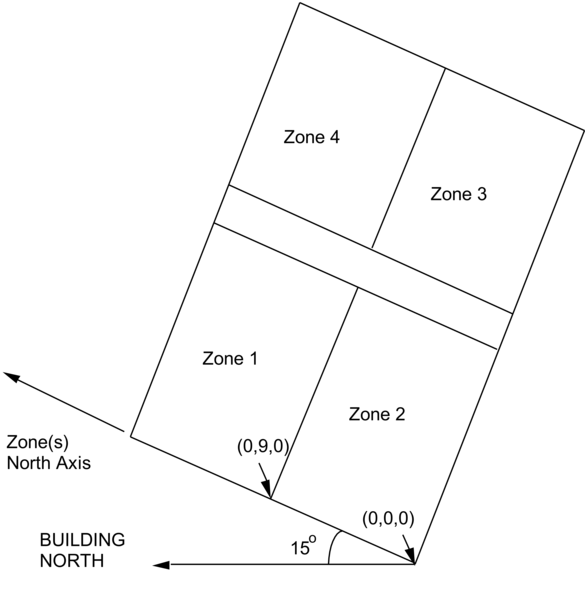
\includegraphics[width=0.9\textwidth, height=0.9\textheight, keepaspectratio=true]{media/image053.png}
\caption{Illustration of Zone North Axis and Origins \protect \label{fig:illustration-of-zone-north-axis-and-origins}}
\end{figure}

\paragraph{Field: Type}\label{field-type-000}

Zone type is currently unused.

\paragraph{Field: Multiplier}\label{field-multiplier}

Zone Multiplier is designed as a ``multiplier'' for floor area, zone loads, and energy consumed by internal gains. It takes the calculated load for the zone and multiplies it, sending the multiplied load to the attached HVAC system. The HVAC system size is specified to meet the entire multiplied zone load and will report the amount of the load met in the Zone Air System Sensible Heating or Cooling Energy/Rate output variable. Autosizing automatically accounts for multipliers. Metered energy consumption by internal gains objects such as Lights or Electric Equipment will be multiplied. The default is 1.

\paragraph{Field: Ceiling Height}\label{field-ceiling-height}

Zone ceiling height is used in several areas within EnergyPlus (such as various room models, some convection coefficient calculations and, primarily, in calculating zone volume in the absence of other parameters). Energyplus automatically calculates the zone ceiling height (m) from the average height of the zone. If this field is 0.0, negative or \textbf{autocalculate}, then the calculated zone ceiling height will be used in subsequent calculations. If this field is positive, then the calculated zone ceiling height will not be used -- the number entered here will be used as the zone ceiling height. If this number differs significantly from the calculated ceiling height, then a warning message will be issued. If a zone ceiling height is entered, but no Volume is entered, then the floor area (if there is one) times the zone ceiling height will be used as the volume.

Note that the Zone Ceiling Height is the distance from the Floor to the Ceiling in the Zone, not an absolute height from the ground.

\paragraph{Field: Volume}\label{field-volume}

Zone volume is used in several areas within EnergyPlus (such as calculating air change rates for reporting or flow when air change rates are chosen as input, daylighting calculations, some convection coefficient calculations). EnergyPlus automatically calculates the zone volume (m\(^{3}\)) from the zone geometry given by the surfaces that belong to the zone. If this field is 0.0, negative or \textbf{autocalculate}, then the calculated zone volume will be used in subsequent calculations. If this field is positive, then it will be used as the zone volume. If this number differs significantly from the calculated zone volume a warning message will be issued. For autocalculate to work properly, the zone must be enclosed by the entered walls. Note that indicating the volume to be calculated but entering a positive ceiling height in the previous field will cause the volume to be calculated as the floor area (if \textgreater{} 0) times the entered ceiling height; else the volume will be calculated from the described surfaces. If this field is positive, any ceiling height positive value will not be used in volume calculations.

\paragraph{Field: Floor Area}\label{field-floor-area}

Zone floor area is used in many places within EnergyPlus. EnergyPlus automatically calculates the zone floor area (m\(^{2}\)) from the zone geometry given by the surfaces that belong to the zone. If this field is 0.0, negative or \textbf{autocalculate}, then the calculated zone floor area will be used in subsequent calculations. If this field is positive, then it will be used as the zone floor area. If this number differs significantly from the calculated zone floor area a warning message will be issued.

\paragraph{Field: Zone Inside Convection Algorithm}\label{field-zone-inside-convection-algorithm}

The Zone Inside Convection Algorithm field is optional. This field specifies the convection model to be used for the inside face of heat transfer surfaces associated with this zone. The choices are: \textbf{Simple} (constant natural convection - ASHRAE), \textbf{TARP} (combines natural and wind-driven convection correlations from laboratory measurements on flat plates), \textbf{CeilingDiffuser} (ACH based forced and mixed convection correlations for ceiling diffuser configuration with simple natural convection limit), \textbf{AdaptiveConvectionAlgorithm} (complex arrangement of various models that adapt to various zone conditions and can be customized) and \textbf{TrombeWall} (variable natural convection in an enclosed rectangular cavity). See the Inside Convection Algorithm object for further descriptions of the available models.

If omitted or blank, the algorithm specified in the SurfaceConvectionAlgorithm:Inside object is the default.

\paragraph{Field: Zone Outside Convection Algorithm}\label{field-zone-outside-convection-algorithm}

The Zone Outside Convection Algorithm field is optional. This field specifies the convection model to be used for the outside face of heat transfer surfaces associated with this zone. The choices are: \textbf{SimpleCombined}, \textbf{TARP}, \textbf{DOE-2}, \textbf{MoWiTT, and AdaptiveConvectionAlgorithm}. The simple convection model applies heat transfer coefficients depending on the roughness and windspeed. This is a combined heat transfer coefficient that includes radiation to sky, ground, and air. The correlation is based on Figure~\ref{fig:schematic-of-the-energyplus-unitary-system}, Page 25.1 (Thermal and Water Vapor Transmission Data), 2001 ASHRAE Handbook of Fundamentals.

The other convection models apply heat transfer coefficients depending on the roughness, windspeed, and terrain of the building's location. These are \emph{convection only} heat transfer coefficients; radiation heat transfer coefficients are calculated automatically by the program. The TARP algorithm was developed for the TARP software and combines natural and wind-driven convection correlations from laboratory measurements on flat plates. The DOE-2 and MoWiTT were derived from field measurements. The AdaptiveConvectionAlgorithm model is an dynamic algorithm that organizes a large number of different convection models and automatically selects the one that best applies. The adaptive convection algorithm can also be customized using the SurfaceConvectionAlgorithm:Outside:AdaptiveModelSelections input object. All algorithms are described more fully in the Engineering Reference.

If omitted or blank, the algorithm specified in the SurfaceConvectionAlgorithm:Outside object is the default.

\paragraph{Field: Part of Total Floor Area}\label{field-part-of-total-floor-area}

This optional field defaults to Yes if not specified. The field is used to show when a zone is not part of the Total Floor Area as shown in the Annual Building Utility Performance Summary tables. Specifically, when No is specified, the area is excluded from both the conditioned floor area and the total floor area in the Building Area sub table and the Normalized Metrics sub tables.

And, an IDF example:

\begin{lstlisting}

  Zone,
      DORM ROOMS AND COMMON AREAS,  !- Name
      0.0000000E+00,           !- Direction of Relative North {deg}
      0.0000000E+00,           !- X Origin {m}
      6.096000,                !- Y Origin {m}
      0.0000000E+00,           !- Z Origin {m}
      1,                       !- Type
      1,                       !- Multiplier
      autocalculate,           !-Ceiling Height {m}
      autocalculate;           !- Volume {m3}
\end{lstlisting}

\subsubsection{Outputs}\label{outputs-037}

\begin{itemize}
\item
  Zone,Average,Zone Outdoor Air Drybulb Temperature {[}C{]}
\item
  Zone,Average,Zone Outdoor Air Wetbulb Temperature {[}C{]}
\item
  Zone,Average,Zone Outdoor Air Wind Speed {[}m/s{]}
\end{itemize}

\paragraph{Zone Outdoor Air Drybulb Temperature {[}C{]}}\label{zone-outdoor-air-drybulb-temperature-c-000}

The outdoor air dry-bulb temperature calculated at the height above ground of the zone centroid.

\paragraph{Zone Outdoor Air Wetbulb Temperature {[}C{]}}\label{zone-outdoor-air-wetbulb-temperature-c-000}

The outdoor air wet-bulb temperature calculated at the height above ground of the zone centroid.

\paragraph{Zone Outdoor Air Wind Speed {[}m/s{]}}\label{zone-outdoor-air-wind-speed-ms-000}

The outdoor wind speed calculated at the height above ground of the zone centroid.

\subsection{Zone Thermal Output(s)}\label{zone-thermal-outputs}

In addition to the canned Surface reports (view the Reports section later in this document) and surface variables (above), the following variables are available for all zones:

\begin{itemize}
\item
  Zone,Sum,Zone Total Internal Radiant Heating Energy {[}J{]}
\item
  Zone,Average,Zone Total Internal Radiant Heating Rate {[}W{]}
\item
  Zone,Sum,Zone Total Internal Visible Radiation Heating Energy {[}J{]}
\item
  Zone,Average,Zone Total Internal Visible Radiation Heating Rate {[}W{]}
\item
  Zone,Sum,Zone Total Internal Convective Heating Energy {[}J{]}
\item
  Zone,Average,Zone Total Internal Convective Heating Rate {[}W{]}
\item
  Zone,Sum,Zone Total Internal Latent Gain Energy {[}J{]}
\item
  Zone,Average,Zone Total Internal Latent Gain Rate {[}W{]}
\item
  Zone,Sum,Zone Total Internal Total Heating Energy {[}J{]}
\item
  Zone,Average,Zone Total Internal Total Heating Rate {[}W{]}
\item
  Zone,Average,Zone Mean Air Temperature {[}C{]}
\item
  HVAC,Average,Zone Air Temperature {[}C{]}
\item
  Zone,Average,Zone Mean Air Dewpoint Temperature {[}C{]}
\item
  Zone,Average,Zone Mean Radiant Temperature {[}C{]}
\item
  Zone,Average,Zone Operative Temperature {[}C{]}
\item
  HVAC,Average,Zone Air Heat Balance Internal Convective Heat Gain Rate {[}W{]}
\item
  HVAC,Average,Zone Air Heat Balance Surface Convection Rate {[}W{]}
\item
  HVAC,Average,Zone Air Heat Balance Interzone Air Transfer Rate {[}W{]}
\item
  HVAC,Average,Zone Air Heat Balance Outdoor Air Transfer Rate {[}W{]}
\item
  HVAC,Average,Zone Air Heat Balance System Air Transfer Rate {[}W{]}
\item
  HVAC,Average,Zone Air Heat Balance System Convective Heat Gain Rate {[}W{]}
\item
  HVAC,Average,Zone Air Heat Balance Air Energy Storage Rate {[}W{]}
\item
  HVAC,Average,Zone Air Heat Balance Deviation Rate {[}W{]}
\item
  HVAC,Sum,Zone Air System Sensible Heating Energy {[}J{]}
\item
  HVAC,Sum,Zone Air System Sensible Cooling Energy {[}J{]}
\item
  HVAC,Average,Zone Air System Sensible Heating Rate {[}W{]}
\item
  HVAC,Average,Zone Air System Sensible Cooling Rate {[}W{]}
\item
  HVAC,Average,Zone Air Humidity Ratio{[}kgWater/kgDryAir{]}
\item
  HVAC,Average,Zone Air Relative Humidity{[}\%{]}
\end{itemize}

Two of these are of particular interest:

\begin{lstlisting}
Zone,Average,Zone Mean Air Temperature [C]
HVAC,Average,Zone Air Temperature [C]
\end{lstlisting}

These two variable outputs are/should be identical. However, note that they can be reported at different time intervals. ``Zone Mean Air Temperature'' is only available on the Zone/HB timestep (Number of Timesteps per Hour) whereas ``Zone Air Temperature'' can be reported at the HVAC timestep (which can vary).

\subsubsection{Zone Mean Air Temperature {[}C{]}}\label{zone-mean-air-temperature-c}

From the code definition, the zone mean air temperature is the average temperature of the air temperatures at the system timestep. Remember that the zone heat balance represents a ``well stirred'' model for a zone, therefore there is only one mean air temperature to represent the air temperature for the zone.

\subsubsection{Zone Air Temperature {[}C{]}}\label{zone-air-temperature-c}

This is very similar to the mean air temperature in the last field. The ``well stirred'' model for the zone is the basis, but this temperature is also available at the ``detailed'' system timestep.

\subsubsection{Zone Mean Air Dewpoint Temperature {[}C{]}}\label{zone-mean-air-dewpoint-temperature-c}

This is the dewpoint temperature of the zone calculated from the Zone Mean Air Temperature (above), the Zone Air Humidity Ratio (below) and the outdoor barometric pressure.

\subsubsection{Zone Thermostat Air Temperature {[}C{]}}\label{zone-thermostat-air-temperature-c}

This is the zone air node temperature for the well-mixed room air model, which is the default room air model type (RoomAirModelType = Mixing). But for other types of Room Air Model (the RoomAir:TemperaturePattern:* and RoomAirSettings:* objects) the zone thermostat air temperature may depend on the Thermostat Height and Thermostat Offset.

\subsubsection{Zone Mean Radiant Temperature {[}C{]}}\label{zone-mean-radiant-temperature-c}

The Mean Radiant Temperature (MRT) in degrees Celsius of a space is a measure of the combined effects of temperatures of surfaces within that space. Specifically it is the surface area × emissivity weighted average of the zone inside surface temperatures (ref. Surface Inside Temperature), where emissivity is the Thermal Absorptance of the inside material layer of each surface.

\subsubsection{Zone Operative Temperature {[}C{]}}\label{zone-operative-temperature-c}

Zone Operative Temperature (OT) is the average of the Zone Mean Air Temperature (MAT) and Zone Mean Radiant Temperature (MRT), OT = 0.5*MAT + 0.5*MRT. This output variable is not affected by the type of thermostat controls in the zone, and does not include the direct effect of high temperature radiant systems. See also Zone Thermostat Operative Temperature.

\subsubsection{Zone Air Heat Balance Internal Convective Heat Gain Rate {[}W{]}}\label{zone-air-heat-balance-internal-convective-heat-gain-rate-w}

The Zone Air Heat Balance Internal Convective Heat Gain Rate is the sum, in watts, of heat transferred to the zone air from all types of internal gains, including people, lights, equipment etc. This and the following provide results on the load components of the zone air heat balance. This field is not multiplied by zone or group multipliers.

\subsubsection{Zone Air Heat Balance Surface Convection Rate {[}W{]}}\label{zone-air-heat-balance-surface-convection-rate-w}

The Zone Air Heat Balance Surface Convection Rate is the sum, in watts, of heat transferred to the zone air from all the surfaces. This field is not multiplied by zone or group multipliers.

\subsubsection{Zone Air Heat Balance Interzone Air Transfer Rate {[}W{]}}\label{zone-air-heat-balance-interzone-air-transfer-rate-w}

The Zone Air Heat Balance Interzone Air Transfer Rate is the sum, in watts, of heat transferred to the zone air from all the transfers of air from other thermal zones. This field is not multiplied by zone or group multipliers.

\subsubsection{Zone Air Heat Balance Outdoor Air Transfer Rate {[}W{]}}\label{zone-air-heat-balance-outdoor-air-transfer-rate-w}

The Zone Air Heat Balance Outdoor Air Transfer Rate is the sum, in watts, of heat transferred to the zone air from all the transfers of air from the out side, such as infiltration. This field is not multiplied by zone or group multipliers.

\subsubsection{Zone Air Heat Balance System Air Transfer Rate {[}W{]}}\label{zone-air-heat-balance-system-air-transfer-rate-w}

The Zone Air Heat Balance System Air Transfer Rate is the sum, in watts, of heat transferred to the zone air by HVAC forced-air systems and air terminal units. Such HVAC systems are connected to the zone by an inlet node (see ZoneHVAC:EquipmentConnections input field called Zone Air Inlet Node or Node List Name) This field is not multiplied by zone or group multipliers. The Zone Air Heat Balance System Air Transfer Rate may not agree exactly with the equipment-level delivered energy transfer rate when the zone temperature is changing significantly over a timestep (e.g. during thermostat setback and setup), but the energy will balance out over time. 

\subsubsection{Zone Air Heat Balance System Convective Heat Gain Rate {[}W{]}}\label{zone-air-heat-balance-system-convective-heat-gain-rate-w}

The Zone Air Heat Balance System Convective Heat Gain Rate is the sum, in watts, of heat transferred directly to the zone air by ``non-air'' HVAC systems. Such HVAC systems are not connected to the zone by an inlet node but rather add or subtract heat directly to the zone air in a manner similar to internal gains. These include the convective fraction of zone HVAC baseboards and high temperature radiant systems, zone HVAC refrigeration chiller set, and the extra convective cooling provided by the cooled beam air terminal unit. This field is not multiplied by zone or group multipliers.

\subsubsection{Zone Air Heat Balance Air Energy Storage Rate {[}W{]}}\label{zone-air-heat-balance-air-energy-storage-rate-w}

The Zone Air Heat Balance Air Energy Storage Rate is the heat stored, in watts, in the zone air as result of zone air temperature changing from one timestep to the next. This field is not multiplied by zone or group multipliers.

\subsubsection{Zone Air Heat Balance Deviation Rate {[}W{]}}\label{zone-air-heat-balance-deviation-rate-w}

The Zone Air Heat Balance Deviation Rate is the imbalance, in watts, in the energy balance for zone air. The value should be near zero but will become non-zero if zone conditions are changing rapidly or erratically. This field is not multiplied by zone or group multipliers. (This output variable is only generated if the user has set a computer system environment variable DisplayAdvancedReportVariables equal to ``yes''.)

\subsubsection{Zone Air System Sensible Heating Energy {[}J{]}}\label{zone-air-system-sensible-heating-energy-j}

This output variable represents the sensible heating energy in Joules that is actually supplied by the system to that zone for the timestep reported. This is the sensible heating rate multiplied by the simulation timestep. This is calculated and reported from the Correct step in the Zone Predictor-Corrector module. This field is not multiplied by zone or group multipliers.

\begin{callout}
Zone Air System Sensible Heating (and Cooling) Energy (and Rate) all report the heating or cooling delivered by the HVAC system to a zone. These values are calculated by multiplying the supply air mass flow rate by the difference between the supply air temperature and the zone air temperature. This does not always indicate the operation of heating or cooling coils. For example, cooling will be reported if the supply air is cooled due to the introduction of outside air, even if all coils are off.

Note that these variables are calculated at the system timestep. When reported at the ``detailed'' reporting frequency, these variable will never show heating and cooling both in the same system timestep. If reported at a frequency less than ``Detailed'' (for example, Hourly) values may appear in both the heating and cooling variable for the same hour if the system cooled the zone for part of the reporting period and heated the zone for another part of the reporting period.
\end{callout}

\subsubsection{Zone Air System Sensible Cooling Energy {[}J{]}}\label{zone-air-system-sensible-cooling-energy-j}

This output variable represents the sensible cooling energy in Joules that is actually supplied by the system to that zone for the timestep reported. This is the sensible cooling rate multiplied by the simulation timestep. This is calculated and reported from the Correct step in the Zone Predictor-Corrector module. This field is not multiplied by zone or group multipliers.

\subsubsection{Zone Air System Sensible Heating Rate {[}W{]}}\label{zone-air-system-sensible-heating-rate-w}

This output variable represents the sensible heating rate in Watts that is actually supplied by the system to that zone for the timestep reported. This is calculated and reported from the Correct step in the Zone Predictor-Corrector module. This field is not multiplied by zone or group multipliers.

\subsubsection{Zone Air System Sensible Cooling Rate {[}W{]}}\label{zone-air-system-sensible-cooling-rate-w}

This output variable represents the sensible cooling rate in Watts that is actually supplied by the system to that zone for the timestep reported. This is calculated and reported from the Correct step in the Zone Predictor-Corrector module. This field is not multiplied by zone or group multipliers.

\subsubsection{Zone Air Humidity Ratio {[}kgWater/kgDryAir{]}}\label{zone-air-humidity-ratio-kgwaterkgdryair}

This output variable represents the air humidity ratio after the correct step for each zone. The humidity ratio is the mass of water vapor to the mass of dry air contained in the zone in (kg water/kg air) and is unitless.

\subsubsection{Zone Air Relative Humidity {[}\%{]}}\label{zone-air-relative-humidity}

This output variable represents the air relative humidity after the correct step for each zone. The relative humidity is in percent and uses the Zone Air Temperature, the Zone Air Humidity Ratio and the Outside Barometric Pressure for calculation.

\subsubsection{Zone Total Internal Radiant Heating Rate {[}W{]}}\label{zone-total-internal-radiant-heating-rate-w}

\subsubsection{Zone Total Internal Radiant Heating Energy {[}J{]}}\label{zone-total-internal-radiant-heating-energy-j}

These output variables represent the sum of radiant gains from specific internal sources (e.g.~equipment) throughout the zone in Watts (for rate) or joules. This includes radiant gain from People, Lights, Electric Equipment, Gas Equipment, Other Equipment, Hot Water Equipment, and Steam Equipment.

\subsubsection{Zone Total Internal Visible Radiation Heating Rate {[}W{]}}\label{zone-total-internal-visible-radiation-heating-rate-w}

\subsubsection{Zone Total Internal Visible Radiation Heating Energy {[}J{]}}\label{zone-total-internal-visible-radiation-heating-energy-j}

These output variables expresse the sum of heat gain in Watts (for rate) or joules that is the calculated short wavelength radiation gain from lights in the zones. This calculation uses the total energy from lights and the fraction visible to realize this value, summed over the zones in the simulation.

\subsubsection{Zone Total Internal Convective Heating Rate {[}W{]}}\label{zone-total-internal-convective-heating-rate-w}

\subsubsection{Zone Total Internal Convective Heating Energy {[}J{]}}\label{zone-total-internal-convective-heating-energy-j}

These output variables represent the sum of convective gains from specific sources (e.g.~equipment) throughout the zone in Watts (for rate) or joules. This includes convective gain from People, Lights, Electric Equipment, Gas Equipment, Other Equipment, Hot Water Equipment, and Steam Equipment.

\subsubsection{Zone Total Internal Latent Gain Rate {[}W{]}}\label{zone-total-internal-latent-gain-rate-w}

\subsubsection{Zone Total Internal Latent Gain Energy {[}J{]}}\label{zone-total-internal-latent-gain-energy-j}

These output variables represent the sum of latent gains from specific internal sources (e.g.~equipment) throughout the zone in Watts (for rate) or joules. This includes latent gain from People, Electric Equipment, Gas Equipment, Other Equipment, Hot Water Equipment, and Steam Equipment.

\subsubsection{Zone Total Internal Total Heating Rate {[}W{]}}\label{zone-total-internal-total-heating-rate-w}

\subsubsection{Zone Total Internal Total Heating Energy {[}J{]}}\label{zone-total-internal-total-heating-energy-j}

These output variables represent the sum of all heat gains throughout the zone in Watts (for rate) or joules. This includes all heat gains from People, Lights, Electric Equipment, Gas Equipment, Other Equipment, Hot Water Equipment, and Steam Equipment.

\subsection{ZoneList}\label{zonelist}

The ZoneList object defines a list of Zone objects. It is primarily used with the ZoneGroup object to provide a generalized way for doing ``Floor Multipliers''. (See the ZoneGroup description below.) The associated ZoneList output variables also provide a way to aggregate and organize zone loads.

Zone lists are not exclusive. A zone can be referenced be more than one ZoneList object.

\subsubsection{Inputs}\label{inputs-1-045}

\paragraph{Field: Zone List Name}\label{field-zone-list-name-000}

The name of the ZoneList object. Must be unique across ZoneLists.

\paragraph{Field: Zone 1 - Zone 20 Name}\label{field-zone-1---zone-20-name}

Reference to a Zone object. This field is extensible; for greater than 20 zones, edit the IDD to add more \emph{Zone Name} fields.

\begin{lstlisting}

ZoneList,
  Mid Floor List,  !- Name
  Mid West Zone,   !- Zone 1 Name
  Mid Center Zone, !- Zone 2 Name
  Mid East Zone;   !- Zone 3 Name
\end{lstlisting}

\subsubsection{Outputs}\label{outputs-1-028}

The following output variables are reported by the ZoneList object:

\begin{itemize}
\item
  HVAC,Average,Zone List Sensible Heating Rate {[}W{]}
\item
  HVAC,Average,Zone List Sensible Cooling Rate {[}W{]}
\item
  HVAC,Sum,Zone List Sensible Heating Energy {[}J{]}
\item
  HVAC,Sum,Zone List Sensible Cooling Energy {[}J{]}
\end{itemize}

All ZoneList variables are the sum of the corresponding Zone variables. \emph{Zone Multiplier} fields in the Zone objects are also taken into account.

\subsection{ZoneGroup}\label{zonegroup}

The ZoneGroup object adds a multiplier to a ZoneList. This can be used to reduce the amount of input necessary for simulating repetitive structures, such as the identical floors of a multi-story building. To create a ``Floor Multiplier'', use the ZoneList object to organize several zones into a typical floor. Then use the \emph{Zone List Multiplier} field in the ZoneGroup object to multiply the system load for the zones in the list will also be multiplied. Zones with a \emph{Multiplier} field greater than one in the Zone object are effectively double-multiplied.

\begin{callout}
NOTE: Although ZoneLists are not exclusive by themselves, ZoneLists used to form a ZoneGroup are exclusive; the ZoneLists used with a ZoneGroup must not have any zones in common.
\end{callout}

\subsubsection{Inputs}\label{inputs-2-042}

\paragraph{Tips for Multi-Story Simulations:}\label{tips-for-multi-story-simulations}

\begin{itemize}
\item
  For floors that are multiplied, connect exterior boundary conditions of the floor to the ceiling and vice versa.
\item
  Since exterior convection coefficients vary with elevation, locate the typical middle floor zones mid-height between the lowest and highest middle floors to be modeled.
\item
  Shading must be identical for all multiplied floors or less accurate results may be obtained by using the zone list multiplier.
\end{itemize}

ZoneGroup and ZoneList can also be used to simulate other repetitive cases, such as clusters of zones on the ground.

\paragraph{Field: Zone Group Name}\label{field-zone-group-name}

The name of the ZoneGroup object. This must be unique across ZoneGroups.

\paragraph{Field: Zone List Name}\label{field-zone-list-name-1}

Reference to a ZoneList object. The zones in the list constitute the zones in the group.

\paragraph{Field: Zone List Multiplier}\label{field-zone-list-multiplier}

An integer multiplier. Zone List Multiplier is designed as a ``multiplier'' for floor area, zone loads, and energy consumed by internal gains. It takes the calculated load for the zone and multiplies it, sending the multiplied load to the attached HVAC system. The HVAC system size is specified to meet the entire multiplied zone load and will report the amount of the load met in the Zone Air System Sensible Heating or Cooling Energy/Rate output variable. Autosizing automatically accounts for multipliers. Metered energy consumption by internal gains objects such as Lights or Electric Equipment will be multiplied. The default is 1.

\begin{lstlisting}

ZONE GROUP,
    Mid Floor,  !- Zone Group Name
    Mid Floor List,  !- Zone List Name
    8;  !- Zone List Multiplier
\end{lstlisting}

\subsubsection{Outputs}\label{outputs-2-023}

The following output variables are reported by the ZoneGroup object:

\begin{itemize}
\item
  HVAC,Average,Zone Group Sensible Heating Rate {[}W{]}
\item
  HVAC,Average,Zone Group Sensible Cooling Rate {[}W{]}
\item
  HVAC,Sum,Zone Group Sensible Heating Energy {[}J{]}
\item
  HVAC,Sum,Zone Group Sensible Cooling Energy {[}J{]}
\end{itemize}

All ZoneGroup variables report the associated ZoneList value multiplied by the \emph{Zone List Multiplier}.

\subsection{Surface(s)}\label{surfaces}

What's a building without surfaces?

EnergyPlus allows for several surface types:

\begin{itemize}
\item
  \textbf{BuildingSurface:Detailed}
\item
  \textbf{FenestrationSurface:Detailed}
\item
  \textbf{Shading:Site:Detailed}
\item
  \textbf{Shading:Building:Detailed}
\item
  \textbf{Shading:Zone:Detailed}
\end{itemize}

Each of the preceding surfaces has ``correct'' geometry specifications. BuildingSurface and Fenestration surfaces (heat transfer surfaces) are used to describe the important elements of the building (walls, roofs, floors, windows, doors) that will determine the interactions of the building surfaces with the outside environment parameters and the internal space requirements. These surfaces are also used to represent ``interzone'' heat transfer. All surfaces are modeled as a thin plane (with no thickness) except that material thicknesses are taken into account for heat transfer calculations.

During specification of surfaces, several ``outside'' environments may be chosen:

\begin{itemize}
\item
  \textbf{Ground} -- when the surface is in touch with the ground (e.g.~slab floors)
\item
  \textbf{Outdoors} -- when the surface is an external surface (e.g.~walls, roofs, windows directly exposed to the outdoor conditions)
\item
  \textbf{Surface} -- when the surface is
  \begin{itemize}
    \item
      An adiabatic internal zone surface
    \item
      A interzone surface
  \end{itemize}
\item
  \textbf{Zone --} when the surface is
  \begin{itemize}
    \item
      A interzone surface in which the other surface is not put in the input file.
  \end{itemize}
\item
  \textbf{OtherSideCoefficients} -- when using a custom profile to describe the external conditions of the surface (advanced concept -- covered in subject: SurfaceProperty:OtherSideCoefficients)
\item
  \textbf{OtherSideConditionsModel} -- when using specially modeled components, such as active solar systems, that cover the outside surface and modify the conditions it experiences.
\end{itemize}

\textbf{Surface} items must also specify an ``outside face object''. This is

\begin{itemize}
\tightlist
\item
  Current surface name -- for adiabatic internal surfaces.
\item
  A surface name in another zone -- for interzone heat transfer.
\item
  An ``opposing'' surface name (in the current zone) -- for representing ``middle'' zones.
\end{itemize}

\textbf{Zone} items must also specify an ``outside face object''. This is

\begin{itemize}
\tightlist
\item
  The zone that contains the other surface that is adjacent to this surface but is not entered in input.
\end{itemize}

\begin{callout}
Note that heat transfer surfaces are fully represented with each description. As stated earlier in the Construction description, materials in the construction (outside to inside) are included but film coefficients neither inside nor outside are used in the description -- these are automatically calculated during the EnergyPlus run. Interzone surfaces which do not have a symmetrical construction (such as a ceiling/floor) require two Construction objects with the layers in reverse order. For example, CEILING with carpet, concrete, ceiling tile and FLOOR with ceiling tile, concrete, carpet. If interzone surfaces have a symmetrical construction, the specification for the two surfaces can reference the same Construction. When a surface is connected as the outside boundary condition for another surface, the two surfaces may be in the same plane, or they may be separated to imply thickness.
\end{callout}

\textbf{Shading} surfaces are used to describe aspects of the site which do not directly impact the physical interactions of the environmental parameters but may significantly shade the building during specific hours of the day or time so the year (e.g.~trees, bushes, mountains, nearby buildings which aren't being simulated as part of this facility, etc.)

\begin{callout}
Note that surfaces which are part of the simulated building automatically shade other parts of the building as geometry and time of day dictate -- there is no need on the user's part to include surfaces that might be in other zones for shading.
\end{callout}

Another surface type:

\begin{itemize}
\tightlist
\item
  \textbf{InternalMass}
\end{itemize}

is used to specify the construction/material parameters and area of items within the space that are important to heat transfer calculations but not necessarily important geometrically. (For example, furniture within the space -- particularly for large spaces). Internal mass can also be used for internal walls that are not needed (when FullInteriorAndExterior Solar Distribution is in effect) for solar distribution or to represent many, if not all, interior walls when solar is distributed to the floors only.

\subsection{Interzone Surfaces}\label{interzone-surfaces}

EnergyPlus can quite accurately simulate the surface heat exchange between two zones. However, this accuracy is not always required and using interzonal heat transfer does add to the complexity of the calculations -- thus requiring more CPU time to simulate. More information about interzonal heat transfer calculations is contained in the Engineering Reference. Some simple guidelines are presented here -- for three cases: adiabatic surfaces, surfaces in ``middle'' zones, and surfaces where heat transfer is ``expected'' (e.g.~between a residence and an unheated, attached garage).

\begin{itemize}
\item
  Adiabatic Surfaces -- These surfaces would be represented as common surfaces (between two zones) where both zones are typically the same temperature. Thus, no transfer is expected in the surface from one zone to the next. These surfaces should be described as simply internal surfaces for the zone referencing as their Outside Boundary Condition Object (see later description in individual surface objects) their own surface names.
\item
  Surfaces in Middle Zones -- Middle zones in a building can be simulated using a judicious use of surfaces and zone multipliers to effect the correct ``loads'' for the building. Thus, middle zone behavior can be simulated without modeling the adjacent zones. This is done by specifying a surface within the zone. For example, a middle floor zone can be modeled by making the floor the Outside Boundary Condition Object for the ceiling, and the ceiling the Outside Boundary Condition Object for the floor.
\item
  Surfaces between Zones with differing temperatures -- These zones represent the true use of interzone surfaces. In a residence that has an attached garage, the garage may be unheated/uncooled or at least not conditioned to the same degree as the residence interior. In this case, EnergyPlus can be used to accurately calculate the effects of the differently conditioned space to the other spaces.
\end{itemize}

\subsection{Surface View Factors}\label{surface-view-factors}

EnergyPlus uses an area weighted approximation to calculate ``view factors'' between surfaces within a thermal zone. Each surface uses the total area that it can ``see'' among the other surfaces. The approximate view factor from this surface to each other surface is then the area of the receiving surface over the sum of areas that is visible to the sending surface.

In order to account in some limited way for the fact that certain surfaces will not see each other, several assumptions have been built into this simple view factor approximation. First, a surface cannot see itself. Second, surfaces with approximately the same azimuth (facing direction) and tilt (``same'' being within a built in limit) will not see each other. This means that a window will not see the wall that it is placed on, for example. Third, floors cannot see each other. Fourth, if the surface is a floor, ceiling, roof, or internal mass, the rule for the same azimuth and tilt eliminating radiant exchange between surface is waived when the receiving surface is floor, roof, ceiling, or internal mass as long as both surfaces are not floors.

Note that this does not take into account that surfaces may be ``around the corner'' from each other and in reality not see each other at all. Rooms are assumed to be convex rather than concave in this method.

To summarize, using the Surface ``Class'', the approximate view factors have:

\begin{enumerate}
\item
  No surface sees itself.
\item
  No Floor sees another floor.
\item
  All other surface types see Internal Mass.
\item
  All other surface types see floors.
\item
  Floors always see ceilings.
\item
  Floors always see roofs.
\item
  All other surfaces whose tilt or facing angle differences are greater than 10 degrees see each other.
\end{enumerate}

If geometry is correct, conditions 1, 3, and 7 should take care of all surfaces, but the other conditions supply common sense when the geometry is incorrect. More information about the EnergyPlus view factor calculation is contained in the Engineering Reference document.

\subsection{GlobalGeometryRules}\label{globalgeometryrules}

Before the surface objects are explained in detail, a description of geometric parameters used in EnergyPlus will be given. Since the input of surface vertices is common to most of the surface types, it will also be given a separate discussion.

Some flexibility is allowed in specifying surface vertices. This flexibility is embodied in the GlobalGeometryRules class/object in the input file. Note that the parameters specified in this statement are used for all surface vertice inputs -- there is no further ``flexibility'' allowed.

In order to perform shadowing calculations, the building surfaces must be specified. EnergyPlus uses a three dimensional (3D) Cartesian coordinate system for surface vertex specification. This Right Hand coordinate system has the X-axis pointing east, the Y-axis pointing north, and the Z-axis pointing up. See figure below.

\begin{figure}[hbtp] % fig 28
\centering
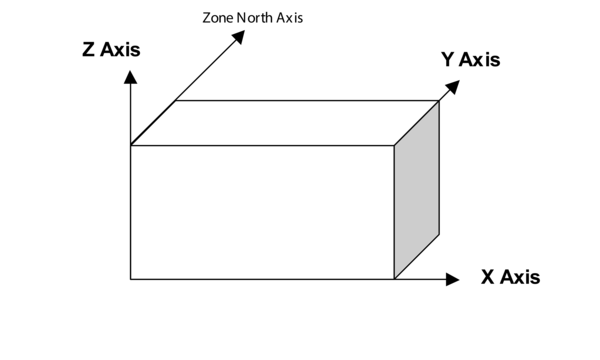
\includegraphics[width=0.9\textwidth, height=0.9\textheight, keepaspectratio=true]{media/image054.png}
\caption{EnergyPlus Coordinate System \protect \label{fig:energyplus-coordinate-system}}
\end{figure}

\subsubsection{Inputs}\label{inputs-3-038}

\paragraph{Field: Starting Vertex Position}\label{field-starting-vertex-position}

The shadowing algorithms in EnergyPlus rely on surfaces having vertices in a certain order and positional structure. Thus, the surface translator needs to know the starting point for each surface entry. The choices are: UpperLeftCorner, LowerLeftCorner , UpperRightCorner, or LowerRightCorner. Since most surfaces will be 4 sided, the convention will specify this position as though each surface were 4 sided. Extrapolate 3 sided figures to this convention. For 5 and more sided figures, again, try to extrapolate the best ``corner'' starting position.

\paragraph{Field: Vertex Entry Direction}\label{field-vertex-entry-direction}

Surfaces are always specified as being viewed from the outside of the zone to which they belong. (Shading surfaces are specified slightly differently and are discussed under the particular types). EnergyPlus needs to know whether the surfaces are being specified in counterclockwise or clockwise order (from the Starting Vertex Position). EnergyPlus uses this to determine the outward facing normal for the surface (which is the \emph{facing angle} of the surface -- very important in shading and shadowing calculations.

\paragraph{Field: Coordinate System}\label{field-coordinate-system}

Vertices can be specified in two ways: using ``Absolute''/``World'' coordinates, or a \textbf{relative} coordinate specification. Relative coordinates allow flexibility of rapid change to observe changes in building results due to orientation and position. ``World'' coordinates will facilitate use within a CADD system structure.

\textbf{Relative} coordinates make use of both Building and Zone North Axis values as well as Zone Origin values to locate the surface in 3D coordinate space. \textbf{World} coordinates do not use these values.

Typically, all zone origin values for ``World'' coordinates will be (0,0,0) but Building and Zone North Axis values may be used in certain instances (namely the Daylighting Coordinate Location entries).

\paragraph{Field: Daylighting Reference Point Coordinate System}\label{field-daylighting-reference-point-coordinate-system}

Daylighting reference points need to be specified as well. Again, there can be two flavors; \textbf{relative} and \textbf{world}. Daylighting reference points must fit within the zone boundaries.

\textbf{Relative} coordinates make use of both Building and Zone North Axis values as well as Zone Origin values to locate the reference point in 3D coordinate space. \textbf{World} coordinates do not use these values.

\paragraph{Field: Rectangular Surface Coordinate System}\label{field-rectangular-surface-coordinate-system}

Simple, rectangular surfaces (Wall:Exterior, Wall:Adiabatic, Wall:Underground, Wall:Interzone, Roof, Ceiling:Adiabatic, Ceiling:Interzone, Floor:GroundContact, Floor:Adiabatic, Floor:Interzone) can be specified with their Lower Left Corner as \textbf{relative} or \textbf{world}.

\textbf{Relative} (default) corners are specified relative to the Zone Origin for each surface. \textbf{World} corners would specify the absolute/world coordinate for this corner.

\subsection{Surfaces}\label{surfaces-1}

Surfaces make up the buildings and the elements that shade buildings. There are several methods to inputting surfaces, ranging from simple rectangular surfaces to detailed descriptions that describe each vertex in the order specified in the GlobalGeometryRules object. The simple, rectangular surface objects are described first with the more detailed descriptions following.

\subsection{Walls}\label{walls}

Walls are usually vertical (tilt = 90 degrees). These objects are used to describe exterior walls, interior walls (adiabatic), underground walls, and walls adjacent to other zones.

\subsection{Wall:Exterior}\label{wallexterior}

The Wall:Exterior object is used to describe walls that are exposed to the external environment. They receive sun, wind -- all the characteristics of the external world.

\subsubsection{Inputs}\label{inputs-4-035}

\paragraph{Field: Name}\label{field-name-047}

This is a unique name associated with the exterior wall. It is used in several other places as a reference (e.g.~as the base surface name for a Window or Door).

\paragraph{Field: Construction Name}\label{field-construction-name-003}

This is the name of the construction (ref: Construction object) used in the surface. Regardless of location in the building, the ``full'' construction (all layers) is used. For example, for an interior wall separating two zones, zone x would have the outside layer (e.g.~drywall) as the material that shows in zone y and then the layers to the inside layer -- the material that shows in zone x. For symmetric constructions, the same construction can be used in the surfaces described in both zones.

\paragraph{Field: Zone Name}\label{field-zone-name-012}

This is the zone name to which the surface belongs.

\paragraph{Field: Azimuth Angle}\label{field-azimuth-angle}

The Azimuth Angle indicates the direction that the wall faces (outward normal). The angle is specified in degrees where East = 90, South = 180, West = 270, North = 0.

\paragraph{Field: Tilt Angle}\label{field-tilt-angle}

The tilt angle is the angle (in degrees) that the wall is tilted from horizontal (or the ground). Normally, walls are tilted 90 degrees and that is the default for this field.

\begin{callout}
\textbf{Starting Corner for the surface}

The rectangular surfaces specify the lower left corner of the surface for their starting coordinate. This is specified with (x,y,z) and can be relative to the zone origin or in world coordinates, depending on the value for rectangular surfaces specified in the GlobalGeometryRules object.
\end{callout}

\paragraph{Field: Starting X Coordinate}\label{field-starting-x-coordinate}

This field is the X coordinate (in meters).

\paragraph{Field: Starting Y Coordinate}\label{field-starting-y-coordinate}

This field is the Y coordinate (in meters).

\paragraph{Field: Starting Z Coordinate}\label{field-starting-z-coordinate}

This field is the Z coordinate (in meters).

\paragraph{Field: Length}\label{field-length-000}

This field is the length of the wall in meters.

\paragraph{Field: Height}\label{field-height-000}

This field is the height of the wall in meters.

\subsection{Wall:Adiabatic}\label{walladiabatic}

The Wall:Adiabatic object is used to describe interior walls and partitions. Adiabatic walls are used to describe walls next to zones that have the same thermal conditions (thus, no heat transfer).

\subsubsection{Inputs}\label{inputs-5-032}

\paragraph{Field: Name}\label{field-name-1-044}

This is a unique name associated with the interior wall. It is used in several other places as a reference (e.g.~as the base surface name for a Window or Door).

\paragraph{Field: Construction Name}\label{field-construction-name-1-001}

This is the name of the construction (ref: Construction object) used in the surface. Regardless of location in the building, the ``full'' construction (all layers) is used. For example, for an interior wall separating two zones, zone x would have the outside layer (e.g.~drywall) as the material that shows in zone y and then the layers to the inside layer -- the material that shows in zone x. For symmetric constructions, the same construction can be used in the surfaces described in both zones.

\paragraph{Field: Zone Name}\label{field-zone-name-1-009}

This is the zone name to which the surface belongs.

\paragraph{Field: Azimuth Angle}\label{field-azimuth-angle-1}

The Azimuth Angle indicates the direction that the wall faces (outward normal). The angle is specified in degrees where East = 90, South = 180, West = 270, North = 0.

\paragraph{Field: Tilt Angle}\label{field-tilt-angle-1}

The tilt angle is the angle (in degrees) that the wall is tilted from horizontal (or the ground). Normally, walls are tilted 90 degrees and that is the default for this field.

\begin{callout}
\textbf{Starting Corner for the surface}

The rectangular surfaces specify the lower left corner of the surface for their starting coordinate. This is specified with (x,y,z) and can be relative to the zone origin or in world coordinates, depending on the value for rectangular surfaces specified in the GlobalGeometryRules object.
\end{callout}

\paragraph{Field: Starting X Coordinate}\label{field-starting-x-coordinate-1}

This field is the X coordinate (in meters).

\paragraph{Field: Starting Y Coordinate}\label{field-starting-y-coordinate-1}

This field is the Y coordinate (in meters).

\paragraph{Field: Starting Z Coordinate}\label{field-starting-z-coordinate-1}

This field is the Z coordinate (in meters).

\paragraph{Field: Length}\label{field-length-1}

This field is the length of the wall in meters.

\paragraph{Field: Height}\label{field-height-1}

This field is the height of the wall in meters.

\subsection{Wall:Underground}\label{wallunderground}

The Wall:Underground object is used to describe walls with ground contact. The temperature at the outside of the wall is the temperature in the GroundTemperature:BuildingSurface object.

\subsubsection{Inputs}\label{inputs-6-029}

\paragraph{Field: Name}\label{field-name-2-039}

This is a unique name associated with the underground wall. It is used in several other places as a reference (e.g.~as the base surface name for a Window or Door).

\paragraph{Field: Construction Name}\label{field-construction-name-2-001}

This is the name of the construction (ref: Construction object) used in the surface. Regardless of location in the building, the ``full'' construction (all layers) is used. For example, for an interior wall separating two zones, zone x would have the outside layer (e.g.~drywall) as the material that shows in zone y and then the layers to the inside layer -- the material that shows in zone x. For symmetric constructions, the same construction can be used in the surfaces described in both zones. Note that if the construction is \textbf{Construction:CfactorUndergroundWall} then the GroundFCfactoreMethod will be used for this wall.

\paragraph{Field: Zone Name}\label{field-zone-name-2-007}

This is the zone name to which the surface belongs.

\paragraph{Field: Azimuth Angle}\label{field-azimuth-angle-2}

The Azimuth Angle indicates the direction that the wall faces (outward normal). The angle is specified in degrees where East = 90, South = 180, West = 270, North = 0.

\paragraph{Field: Tilt Angle}\label{field-tilt-angle-2}

The tilt angle is the angle (in degrees) that the wall is tilted from horizontal (or the ground). Normally, walls are tilted 90 degrees and that is the default for this field.

\paragraph{Starting Corner for the surface}\label{starting-corner-for-the-surface-2}

The rectangular surfaces specify the lower left corner of the surface for their starting coordinate. This is specified with (x,y,z) and can be relative to the zone origin or in world coordinates, depending on the value for rectangular surfaces specified in the GlobalGeometryRules object.

\paragraph{Field: Starting X Coordinate}\label{field-starting-x-coordinate-2}

This field is the X coordinate (in meters).

\paragraph{Field: Starting Y Coordinate}\label{field-starting-y-coordinate-2}

This field is the Y coordinate (in meters).

\paragraph{Field: Starting Z Coordinate}\label{field-starting-z-coordinate-2}

This field is the Z coordinate (in meters).

\paragraph{Field: Length}\label{field-length-2}

This field is the length of the wall in meters.

\paragraph{Field: Height}\label{field-height-2}

This field is the height of the wall in meters.

\subsection{Wall:Interzone}\label{wallinterzone}

The Wall:Interzone object is used to describe walls adjacent to zones that are significantly different conditions than the zone with this wall.

\subsubsection{Inputs}\label{inputs-7-028}

\paragraph{Field: Name}\label{field-name-3-033}

This is a unique name associated with the interzone wall. It is used in several other places as a reference (e.g.~as the base surface name for a Window or Door).

\paragraph{Field: Construction Name}\label{field-construction-name-3}

This is the name of the construction (ref: Construction object) used in the surface. Regardless of location in the building, the ``full'' construction (all layers) is used. For example, for an interior wall separating two zones, zone x would have the outside layer (e.g.~drywall) as the material that shows in zone y and then the layers to the inside layer -- the material that shows in zone x. For symmetric constructions, the same construction can be used in the surfaces described in both zones.

\paragraph{Field: Zone Name}\label{field-zone-name-3-006}

This is the zone name to which the surface belongs.

\paragraph{Field: Outside Boundary Condition Object}\label{field-outside-boundary-condition-object}

The Outside Boundary Condition Object field is the name of a wall in an adjacent zone or the name of the adjacent zone. If the adjacent zone option is used, the adjacent wall is automatically generated in the adjacent zone. If the surface name is used, it must be in the adjacent zone.

\paragraph{Field: Azimuth Angle}\label{field-azimuth-angle-3}

The Azimuth Angle indicates the direction that the wall faces (outward normal). The angle is specified in degrees where East = 90, South = 180, West = 270, North = 0.

\paragraph{Field: Tilt Angle}\label{field-tilt-angle-3}

The tilt angle is the angle (in degrees) that the wall is tilted from horizontal (or the ground). Normally, walls are tilted 90 degrees and that is the default for this field.

\paragraph{Starting Corner for the surface}\label{starting-corner-for-the-surface-3}

The rectangular surfaces specify the lower left corner of the surface for their starting coordinate. This is specified with (x,y,z) and can be relative to the zone origin or in world coordinates, depending on the value for rectangular surfaces specified in the GlobalGeometryRules object.

\paragraph{Field: Starting X Coordinate}\label{field-starting-x-coordinate-3}

This field is the X coordinate (in meters).

\paragraph{Field: Starting Y Coordinate}\label{field-starting-y-coordinate-3}

This field is the Y coordinate (in meters).

\paragraph{Field: Starting Z Coordinate}\label{field-starting-z-coordinate-3}

This field is the Z coordinate (in meters).

\paragraph{Field: Length}\label{field-length-3}

This field is the length of the wall in meters.

\paragraph{Field: Height}\label{field-height-3}

This field is the height of the wall in meters.

\subsection{Roofs/Ceilings}\label{roofsceilings}

Roofs and ceilings are, by default, flat (tilt = 0 degrees). These objects are used to describe roofs, interior ceilings (adiabatic) and ceilings adjacent to other zones.

\subsection{Roof}\label{roof}

The Roof object is used to describe roofs that are exposed to the external environment.

\subsubsection{Inputs}\label{inputs-8-026}

\paragraph{Field: Name}\label{field-name-4-030}

This is a unique name associated with the roof. It is used in several other places as a reference (e.g.~as the base surface name for a Window or Door).

\paragraph{Field: Construction Name}\label{field-construction-name-4}

This is the name of the construction (ref: Construction object) used in the surface. Regardless of location in the building, the ``full'' construction (all layers) is used. For example, for an interior wall separating two zones, zone x would have the outside layer (e.g.~drywall) as the material that shows in zone y and then the layers to the inside layer -- the material that shows in zone x. For symmetric constructions, the same construction can be used in the surfaces described in both zones.

\paragraph{Field: Zone Name}\label{field-zone-name-4-006}

This is the zone name to which the surface belongs.

\paragraph{Field: Azimuth Angle}\label{field-azimuth-angle-4}

The Azimuth Angle indicates the direction of the outward normal for the roof. The angle is specified in degrees where East = 90, South = 180, West = 270, North = 0.

\paragraph{Field: Tilt Angle}\label{field-tilt-angle-4}

The tilt angle is the angle (in degrees) that the wall is tilted from horizontal (or the ground). Flat roofs are tilted 0 degrees and that is the default for this field.

\paragraph{Starting Corner for the surface}\label{starting-corner-for-the-surface-4}

The rectangular surfaces specify the lower left corner of the surface for their starting coordinate. This is specified with (x,y,z) and can be relative to the zone origin or in world coordinates, depending on the value for rectangular surfaces specified in the GlobalGeometryRules object.

\paragraph{Field: Starting X Coordinate}\label{field-starting-x-coordinate-4}

This field is the X coordinate (in meters).

\paragraph{Field: Starting Y Coordinate}\label{field-starting-y-coordinate-4}

This field is the Y coordinate (in meters).

\paragraph{Field: Starting Z Coordinate}\label{field-starting-z-coordinate-4}

This field is the Z coordinate (in meters).

\paragraph{Field: Length}\label{field-length-4}

This field is the length of the roof in meters.

\paragraph{Field: Width}\label{field-width}

This field is the width of the roof in meters.

\subsection{Ceiling:Adiabatic}\label{ceilingadiabatic}

The Ceiling:Adiabatic object is used to describe interior ceilings that separate zones of like conditions.

\subsubsection{Inputs}\label{inputs-9-024}

\paragraph{Field: Name}\label{field-name-5-026}

This is a unique name associated with the ceiling. It is used in several other places as a reference (e.g.~as the base surface name for a Window or Door).

\paragraph{Field: Construction Name}\label{field-construction-name-5}

This is the name of the construction (ref: Construction object) used in the surface. Regardless of location in the building, the ``full'' construction (all layers) is used. For example, for an interior wall separating two zones, zone x would have the outside layer (e.g.~drywall) as the material that shows in zone y and then the layers to the inside layer -- the material that shows in zone x. For symmetric constructions, the same construction can be used in the surfaces described in both zones.

\paragraph{Field: Zone Name}\label{field-zone-name-5-005}

This is the zone name to which the surface belongs.

\paragraph{Field: Azimuth Angle}\label{field-azimuth-angle-5}

The Azimuth Angle indicates the direction of the outward normal for the roof. The angle is specified in degrees where East = 90, South = 180, West = 270, North = 0.

\paragraph{Field: Tilt Angle}\label{field-tilt-angle-5}

The tilt angle is the angle (in degrees) that the wall is tilted from horizontal (or the ground). Flat ceilings are tilted 0 degrees and that is the default for this field.

\paragraph{Starting Corner for the surface}\label{starting-corner-for-the-surface-5}

The rectangular surfaces specify the lower left corner of the surface for their starting coordinate. This is specified with (x,y,z) and can be relative to the zone origin or in world coordinates, depending on the value for rectangular surfaces specified in the GlobalGeometryRules object.

\paragraph{Field: Starting X Coordinate}\label{field-starting-x-coordinate-5}

This field is the X coordinate (in meters).

\paragraph{Field: Starting Y Coordinate}\label{field-starting-y-coordinate-5}

This field is the Y coordinate (in meters).

\paragraph{Field: Starting Z Coordinate}\label{field-starting-z-coordinate-5}

This field is the Z coordinate (in meters).

\paragraph{Field: Length}\label{field-length-5}

This field is the length of the ceiling in meters.

\paragraph{Field: Width}\label{field-width-1}

This field is the width of the ceiling in meters.

\subsection{Ceiling:Interzone}\label{ceilinginterzone}

The Ceiling:Interzone object is used to describe interior ceilings that separate zones of differing conditions (and expect heat transfer through the ceiling from the adjacent zone).

\subsubsection{Inputs}\label{inputs-10-022}

\paragraph{Field: Name}\label{field-name-6-024}

This is a unique name associated with the interzone ceiling. It is used in several other places as a reference (e.g.~as the base surface name for a Window or Door).

\paragraph{Field: Construction Name}\label{field-construction-name-6}

This is the name of the construction (ref: Construction object) used in the surface. Regardless of location in the building, the ``full'' construction (all layers) is used. For example, for an interior wall separating two zones, zone x would have the outside layer (e.g.~drywall) as the material that shows in zone y and then the layers to the inside layer -- the material that shows in zone x. For symmetric constructions, the same construction can be used in the surfaces described in both zones.

\paragraph{Field: Zone Name}\label{field-zone-name-6-004}

This is the zone name to which the surface belongs.

\paragraph{Field: Outside Boundary Condition Object}\label{field-outside-boundary-condition-object-1}

The Outside Boundary Condition Object field is the name of a floor in an adjacent zone or the name of the adjacent zone. If the adjacent zone option is used, the adjacent floor is automatically generated in the adjacent zone. If the surface name is used, it must be in the adjacent zone.

\paragraph{Field: Azimuth Angle}\label{field-azimuth-angle-6}

The Azimuth Angle indicates the direction of the outward normal for the roof. The angle is specified in degrees where East = 90, South = 180, West = 270, North = 0.

\paragraph{Field: Tilt Angle}\label{field-tilt-angle-6}

The tilt angle is the angle (in degrees) that the wall is tilted from horizontal (or the ground). Flat ceilings are tilted 0 degrees and that is the default for this field.

\paragraph{Starting Corner for the surface}\label{starting-corner-for-the-surface-6}

The rectangular surfaces specify the lower left corner of the surface for their starting coordinate. This is specified with (x,y,z) and can be relative to the zone origin or in world coordinates, depending on the value for rectangular surfaces specified in the GlobalGeometryRules object.

\paragraph{Field: Starting X Coordinate}\label{field-starting-x-coordinate-6}

This field is the X coordinate (in meters).

\paragraph{Field: Starting Y Coordinate}\label{field-starting-y-coordinate-6}

This field is the Y coordinate (in meters).

\paragraph{Field: Starting Z Coordinate}\label{field-starting-z-coordinate-6}

This field is the Z coordinate (in meters).

\paragraph{Field: Length}\label{field-length-6}

This field is the length of the ceiling in meters.

\paragraph{Field: Width}\label{field-width-2}

This field is the width of the ceiling in meters.

\subsection{Floors}\label{floors}

Floors are, by default, flat (tilt = 180 degrees). These objects are used to describe floors on the ground, interior floors (adiabatic) and floors adjacent to other zones.

\subsection{Floor:GroundContact}\label{floorgroundcontact}

The Floor:GroundContact object is used to describe floors that have ground contact (usually called slabs). The temperature at the outside of the floor is the temperature in the GroundTemperature:BuildingSurface object.

\subsubsection{Inputs}\label{inputs-11-021}

\paragraph{Field: Name}\label{field-name-7-022}

This is a unique name associated with the floor.

\paragraph{Field: Construction Name}\label{field-construction-name-7}

This is the name of the construction (ref: Construction object) used in the surface. Regardless of location in the building, the ``full'' construction (all layers) is used. For example, for an interior wall separating two zones, zone x would have the outside layer (e.g.~drywall) as the material that shows in zone y and then the layers to the inside layer -- the material that shows in zone x. For symmetric constructions, the same construction can be used in the surfaces described in both zones. Note that if the construction is \textbf{Construction:FfactorGroundFloor,} then the GroundFCfactorMethod will be used with this floor.

\paragraph{Field: Zone Name}\label{field-zone-name-7-004}

This is the zone name to which the surface belongs.

\paragraph{Field: Azimuth Angle}\label{field-azimuth-angle-7}

The Azimuth Angle indicates the direction of the outward normal for the roof. The angle is specified in degrees where East = 90, South = 180, West = 270, North = 0.

\paragraph{Field: Tilt Angle}\label{field-tilt-angle-7}

The tilt angle is the angle (in degrees) that the wall is tilted from horizontal (or the ground). Flat floors are tilted 180 degrees and that is the default for this field.

\paragraph{Starting Corner for the surface}\label{starting-corner-for-the-surface-7}

The rectangular surfaces specify the lower left corner of the surface for their starting coordinate. This is specified with (x,y,z) and can be relative to the zone origin or in world coordinates, depending on the value for rectangular surfaces specified in the GlobalGeometryRules object.

\paragraph{Field: Starting X Coordinate}\label{field-starting-x-coordinate-7}

This field is the X coordinate (in meters).

\paragraph{Field: Starting Y Coordinate}\label{field-starting-y-coordinate-7}

This field is the Y coordinate (in meters).

\paragraph{Field: Starting Z Coordinate}\label{field-starting-z-coordinate-7}

This field is the Z coordinate (in meters).

\paragraph{Field: Length}\label{field-length-7}

This field is the length of the floor in meters.

\paragraph{Field: Width}\label{field-width-3}

This field is the width of the floor in meters.

\subsection{Floor:Adiabatic}\label{flooradiabatic}

The Floor:Adiabatic object is used to describe interior floors or floors that you wish to model with no heat transfer from the exterior to the floor.

\subsubsection{Inputs}\label{inputs-12-019}

\paragraph{Field: Name}\label{field-name-8-022}

This is a unique name associated with the floor.

\paragraph{Field: Construction Name}\label{field-construction-name-8}

This is the name of the construction (ref: Construction object) used in the surface. Regardless of location in the building, the ``full'' construction (all layers) is used. For example, for an interior wall separating two zones, zone x would have the outside layer (e.g.~drywall) as the material that shows in zone y and then the layers to the inside layer -- the material that shows in zone x. For symmetric constructions, the same construction can be used in the surfaces described in both zones.

\paragraph{Field: Zone Name}\label{field-zone-name-8-003}

This is the zone name to which the surface belongs.

\paragraph{Field: Azimuth Angle}\label{field-azimuth-angle-8}

The Azimuth Angle indicates the direction of the outward normal for the roof. The angle is specified in degrees where East = 90, South = 180, West = 270, North = 0.

\paragraph{Field: Tilt Angle}\label{field-tilt-angle-8}

The tilt angle is the angle (in degrees) that the wall is tilted from horizontal (or the ground). Flat floors are tilted 180 degrees and that is the default for this field.

\paragraph{Starting Corner for the surface}\label{starting-corner-for-the-surface-8}

The rectangular surfaces specify the lower left corner of the surface for their starting coordinate. This is specified with (x,y,z) and can be relative to the zone origin or in world coordinates, depending on the value for rectangular surfaces specified in the GlobalGeometryRules object.

\paragraph{Field: Starting X Coordinate}\label{field-starting-x-coordinate-8}

This field is the X coordinate (in meters).

\paragraph{Field: Starting Y Coordinate}\label{field-starting-y-coordinate-8}

This field is the Y coordinate (in meters).

\paragraph{Field: Starting Z Coordinate}\label{field-starting-z-coordinate-8}

This field is the Z coordinate (in meters).

\paragraph{Field: Length}\label{field-length-8}

This field is the length of the floor in meters.

\paragraph{Field: Width}\label{field-width-4}

This field is the width of the floor in meters.

\subsection{Floor:Interzone}\label{floorinterzone}

The Floor:Interzone object is used to describe floors that are adjacent to other zones that have differing conditions and you wish to model the heat transfer through the floor.

\subsubsection{Inputs}\label{inputs-13-016}

\paragraph{Field: Name}\label{field-name-9-019}

This is a unique name associated with the floor.

\paragraph{Field: Construction Name}\label{field-construction-name-9}

This is the name of the construction (ref: Construction object) used in the surface. Regardless of location in the building, the ``full'' construction (all layers) is used. For example, for an interior wall separating two zones, zone x would have the outside layer (e.g.~drywall) as the material that shows in zone y and then the layers to the inside layer -- the material that shows in zone x. For symmetric constructions, the same construction can be used in the surfaces described in both zones.

\paragraph{Field: Zone Name}\label{field-zone-name-9-001}

This is the zone name to which the surface belongs.

\paragraph{Field: Outside Boundary Condition Object}\label{field-outside-boundary-condition-object-2}

The Outside Boundary Condition Object field is the name of a ceiling in an adjacent zone or the name of the adjacent zone. If the adjacent zone option is used, the adjacent ceiling is automatically generated in the adjacent zone. If the surface name is used, it must be in the adjacent zone.

\paragraph{Field: Azimuth Angle}\label{field-azimuth-angle-9}

The Azimuth Angle indicates the direction of the outward normal for the roof. The angle is specified in degrees where East = 90, South = 180, West = 270, North = 0.

\paragraph{Field: Tilt Angle}\label{field-tilt-angle-9}

The tilt angle is the angle (in degrees) that the wall is tilted from horizontal (or the ground). Flat floors are tilted 180 degrees and that is the default for this field.

\paragraph{Starting Corner for the surface}\label{starting-corner-for-the-surface-9}

The rectangular surfaces specify the lower left corner of the surface for their starting coordinate. This is specified with (x,y,z) and can be relative to the zone origin or in world coordinates, depending on the value for rectangular surfaces specified in the GlobalGeometryRules object.

\paragraph{Field: Starting X Coordinate}\label{field-starting-x-coordinate-9}

This field is the X coordinate (in meters).

\paragraph{Field: Starting Y Coordinate}\label{field-starting-y-coordinate-9}

This field is the Y coordinate (in meters).

\paragraph{Field: Starting Z Coordinate}\label{field-starting-z-coordinate-9}

This field is the Z coordinate (in meters).

\paragraph{Field: Length}\label{field-length-9}

This field is the length of the floor in meters.

\paragraph{Field: Width}\label{field-width-5}

This field is the width of the floor in meters.

\subsection{Windows/Doors}\label{windowsdoors}

The following window and door objects can be used to specify simple, rectangular doors and windows. In each case, the lower left corner (locator coordinate) of the window or door is specified \textbf{relative} to the surface it is on. Viewing the base surface as a planar surface, base the relative location from the lower left corner of the base surface. Vertex entry description as well as provisions for a few other surface types can be entered with the FenestrationSurface:Detailed object.

\subsection{Window}\label{window}

The Window object is used to place windows on surfaces that can have windows, including exterior walls, interior walls, interzone walls, roofs, floors that are exposed to outdoor conditions, interzone ceiling/floors. These, of course, can be entered using the simple rectangular objects or the more detailed vertex entry objects. Shades and screens may be applied by referencing this subsurface in a window shading control (ref: WindowShadingControl object). To assign a shade to a window or glass door, see WindowMaterial: Shade. To assign a screen, see WindowMaterial:Screen. To assign a blind, see WindowMaterial:Blind. To assign switchable glazing, such as electrochromic glazing, see WindowShadingControl.


\subsubsection{Inputs}\label{inputs-14-016}

\paragraph{Field: Name}\label{field-name-10-018}

This is a unique name associated with the window.

\paragraph{Field: Construction Name}\label{field-construction-name-10}

This is the name of the subsurface's construction (ref: objects: Construction, Construction:WindowDataFile, Construction:ComplexFenestrationState).

For windows, if Construction Name is not found among the constructions on the input (.idf) file, the Window Data File (ref. Construction:WindowDataFile object) will be searched for that Construction Name (see ``Importing Windows from WINDOW''). If that file is not present or if the Construction Name does not match the name of an entry on the file, an error will result. If there is a match, a window construction and its corresponding glass and gas materials will be created from the information read from the file.

\paragraph{Field: Building Surface Name}\label{field-building-surface-name-000}

This is the name of a surface that contains this subsurface. Certain kinds of surfaces may not be allowed to have subsurfaces. For example, a surface in contact with the ground (e.g., Outside Boundary Condition = Ground) cannot contain a window. The window assumes the outward facing angle as well as the tilt angle of the base surface.

\paragraph{Field: Frame and Divider Name}\label{field-frame-and-divider-name}

This field, if not blank, can be used to specify window frame, divider and reveal-surface data (ref: WindowProperty:FrameAndDivider object). It is used only for exterior GlassDoors and rectangular exterior Windows, i.e., those with OutsideFaceEnvironment = Outdoors.

This field should be blank for triangular windows.

\paragraph{Field: Multiplier}\label{field-multiplier-1}

This field is the number of identical items on the base surface. Using Multiplier can save input effort and calculation time. In the calculation the area (and area of frame and divider, if present and surface type is a window) is multiplied by Multiplier. The calculation of shadowing on the subsurfaces (and the calculation of the interior distribution of beam solar radiation transmitted by windows and glass doors) are done for the specified subsurface position and dimensions.

Multiplier should be used with caution. Multiplier \textgreater{} 1 can give inaccurate or nonsensical results in situations where the results are sensitive to window or glass door position. This includes shadowing on the window/glass door, daylighting from the window/glass door, and interior distribution of solar radiation from the window/glass door. In these cases, the results for the single input window/glass door, after multiplication, may not be representative of the results you would get if you entered each of the multiple subsurfaces separately.

If Multiplier \textgreater{} 1, you will get

--a \emph{warning} if Solar Distribution = FullExterior or FullInteriorAndExterior (ref: Building - Field: Solar Distribution), indicating that the shadowing on the input window or the interior solar radiation distribution from the input window may not be representative of the actual group of windows. No warning is issued if Solar Distribution = MinimalShadowing.

--an \emph{error} if the window is an exterior window/glass door in a zone that has a detailed daylighting calculation (Daylighting:Detailed specified for the zone). Since a single window with a multiplier can never give the same daylight illuminance as the actual set of windows, you are not allowed to use Multiplier in this situation.

\paragraph{Starting Corner for the surface}\label{starting-corner-for-the-surface-10}

The rectangular subsurfaces specify the lower left corner of the surface for their starting coordinate. This corner is specified relative to the lower left corner of the base surface by specifying the X and Z values from that corner.

\paragraph{Field: Starting X Coordinate}\label{field-starting-x-coordinate-10}

This field is the X coordinate (in meters).

\paragraph{Field: Starting Z Coordinate}\label{field-starting-z-coordinate-10}

This field is the Z coordinate (in meters).

\paragraph{Field: Length}\label{field-length-10}

This field is the length of the window in meters.

\paragraph{Field: Height}\label{field-height-4}

This field is the height of the window in meters.

\subsection{Door}\label{door}

The Door object is used to place opaque doors on surfaces that can have doors, including exterior walls, interior walls, interzone walls, roofs, floors that are exposed to outdoor conditions, interzone ceiling/floors. These, of course, can be entered using the simple rectangular objects or the more detailed vertex entry objects.

\subsubsection{Inputs}\label{inputs-15-016}

\paragraph{Field: Name}\label{field-name-11-015}

This is a unique name associated with the door.

\paragraph{Field: Construction Name}\label{field-construction-name-11}

This is the name of the subsurface's construction (ref: Construction object)

\paragraph{Field: Building Surface Name}\label{field-building-surface-name-1}

This is the name of a surface that contains this subsurface. Certain kinds of surfaces may not be allowed to have subsurfaces. The door assumes the outward facing angle as well as the tilt angle of the base surface.

\paragraph{Field: Multiplier}\label{field-multiplier-2}

This field is the number of identical items on the base surface. Using Multiplier can save input effort and calculation time. In the calculation the area (and area of frame and divider, if present and surface type is a window) is multiplied by Multiplier. The calculation of shadowing on the subsurfaces (and the calculation of the interior distribution of beam solar radiation transmitted by windows and glass doors) are done for the specified subsurface position and dimensions.

Multiplier should be used with caution. Multiplier \textgreater{} 1 can give inaccurate or nonsensical results in situations where the results are sensitive to window or glass door position. This includes shadowing on the window/glass door, daylighting from the window/glass door, and interior distribution of solar radiation from the window/glass door. In these cases, the results for the single input window/glass door, after multiplication, may not be representative of the results you would get if you entered each of the multiple subsurfaces separately.

If Multiplier \textgreater{} 1, you will get

--a \emph{warning} if Solar Distribution = FullExterior or FullInteriorAndExterior (ref: Building - Field: Solar Distribution), indicating that the shadowing on the input window or the interior solar radiation distribution from the input window may not be representative of the actual group of windows. No warning is issued if Solar Distribution = MinimalShadowing.

--an \emph{error} if the window is an exterior window/glass door in a zone that has a detailed daylighting calculation (Daylighting:Detailed specified for the zone). Since a single window with a multiplier can never give the same daylight illuminance as the actual set of windows, you are not allowed to use Multiplier in this situation.

\paragraph{Starting Corner for the surface}\label{starting-corner-for-the-surface-11}

The rectangular subsurfaces specify the lower left corner of the surface for their starting coordinate. This corner is specified relative to the lower left corner of the base surface by specifying the X and Z values from that corner.

\paragraph{Field: Starting X Coordinate}\label{field-starting-x-coordinate-11}

This field is the X coordinate (in meters).

\paragraph{Field: Starting Z Coordinate}\label{field-starting-z-coordinate-11}

This field is the Z coordinate (in meters).

\paragraph{Field: Length}\label{field-length-11}

This field is the length of the door in meters.

\paragraph{Field: Height}\label{field-height-5}

This field is the height of the door in meters.

\subsection{GlazedDoor}\label{glazeddoor}

The GlazedDoor object is used to place doors on surfaces that can have doors, including exterior walls, interior walls, interzone walls, roofs, floors that are exposed to outdoor conditions, interzone ceiling/floors. These, of course, can be entered using the simple rectangular objects or the more detailed vertex entry objects. Shades and screens may be applied by referencing this subsurface in a window shading control (ref: WindowShadingControl object). To assign a shade to a window or glass door, see WindowMaterial: Shade. To assign a screen, see WindowMaterial:Screen. To assign a blind, see WindowMaterial:Blind. To assign switchable glazing, such as electrochromic glazing, see WindowShadingControl.

\subsubsection{Inputs}\label{inputs-16-012}

\paragraph{Field: Name}\label{field-name-12-012}

This is a unique name associated with the glass door.

\paragraph{Field: Construction Name}\label{field-construction-name-12}

This is the name of the subsurface's construction (ref: objects: Construction, Construction:WindowDataFile, Construction:ComplexFenestrationState).

For windows, if Construction Name is not found among the constructions on the input (.idf) file, the Window Data File (ref. Construction:WindowDataFile object) will be searched for that Construction Name (see ``Importing Windows from WINDOW''). If that file is not present or if the Construction Name does not match the name of an entry on the file, an error will result. If there is a match, a window construction and its corresponding glass and gas materials will be created from the information read from the file.

\paragraph{Field: Building Surface Name}\label{field-building-surface-name-2}

This is the name of a surface that contains this subsurface. Certain kinds of surfaces may not be allowed to have subsurfaces. For example, a surface in contact with the ground (Outside Boundary Condition = Ground) cannot contain a window. The door assumes the outward facing angle as well as the tilt angle of the base surface.

\paragraph{Field: Frame and Divider Name}\label{field-frame-and-divider-name-1}

This field, if not blank, can be used to specify window frame, divider and reveal-surface data (ref: WindowProperty:FrameAndDivider object). It is used only for exterior GlassDoors and rectangular exterior Windows, i.e., those with OutsideFaceEnvironment = Outdoors.

This field should be blank for triangular windows.

\paragraph{Field: Multiplier}\label{field-multiplier-3}

This field is the number of identical items on the base surface. Using Multiplier can save input effort and calculation time. In the calculation the area (and area of frame and divider, if present and surface type is a window) is multiplied by Multiplier. The calculation of shadowing on the subsurfaces (and the calculation of the interior distribution of beam solar radiation transmitted by windows and glass doors) are done for the specified subsurface position and dimensions.

Multiplier should be used with caution. Multiplier \textgreater{} 1 can give inaccurate or nonsensical results in situations where the results are sensitive to window or glass door position. This includes shadowing on the window/glass door, daylighting from the window/glass door, and interior distribution of solar radiation from the window/glass door. In these cases, the results for the single input window/glass door, after multiplication, may not be representative of the results you would get if you entered each of the multiple subsurfaces separately.

If Multiplier \textgreater{} 1, you will get

--a \emph{warning} if Solar Distribution = FullExterior or FullInteriorAndExterior (ref: Building - Field: Solar Distribution), indicating that the shadowing on the input window or the interior solar radiation distribution from the input window may not be representative of the actual group of windows. No warning is issued if Solar Distribution = MinimalShadowing.

--an \emph{error} if the window is an exterior window/glass door in a zone that has a detailed daylighting calculation (Daylighting:Detailed specified for the zone). Since a single window with a multiplier can never give the same daylight illuminance as the actual set of windows, you are not allowed to use Multiplier in this situation.

\paragraph{Starting Corner for the surface}\label{starting-corner-for-the-surface-12}

The rectangular subsurfaces specify the lower left corner of the surface for their starting coordinate. This corner is specified relative to the lower left corner of the base surface by specifying the X and Z values from that corner.

\paragraph{Field: Starting X Coordinate}\label{field-starting-x-coordinate-12}

This field is the X coordinate (in meters).

\paragraph{Field: Starting Z Coordinate}\label{field-starting-z-coordinate-12}

This field is the Z coordinate (in meters).

\paragraph{Field: Length}\label{field-length-12}

This field is the length of the door in meters.

\paragraph{Field: Height}\label{field-height-6}

This field is the height of the door in meters.

\subsection{Window:Interzone}\label{windowinterzone}

The Window:Interzone object is used to place windows on surfaces that can have windows, including interzone walls, interzone ceiling/floors. These, of course, can be entered using the simple rectangular objects or the more detailed vertex entry objects.

\subsubsection{Inputs}\label{inputs-17-010}

\paragraph{Field: Name}\label{field-name-13-011}

This is a unique name associated with the window.

\paragraph{Field: Construction Name}\label{field-construction-name-13}

This is the name of the subsurface's construction (ref: objects: Construction, Construction:WindowDataFile, Construction:ComplexFenestrationState).

For windows, if Construction Name is not found among the constructions on the input (.idf) file, the Window Data File (ref. Construction:WindowDataFile object) will be searched for that Construction Name (see ``Importing Windows from WINDOW''). If that file is not present or if the Construction Name does not match the name of an entry on the file, an error will result. If there is a match, a window construction and its corresponding glass and gas materials will be created from the information read from the file.

\paragraph{Field: Building Surface Name}\label{field-building-surface-name-3}

This is the name of a surface that contains this subsurface. Certain kinds of surfaces may not be allowed to have subsurfaces. For example, a surface in contact with the ground (Outside Boundary Condition = Ground) cannot contain a window. The window assumes the outward facing angle as well as the tilt angle of the base surface.

\paragraph{Field: Outside Boundary Condition Object}\label{field-outside-boundary-condition-object-3}

The Outside Boundary Condition Object field is the name of a window in an adjacent zone or the name of the adjacent zone. If the adjacent zone option is used, the adjacent ceiling is automatically generated in the adjacent zone. If the surface name is used, it must be in the adjacent zone.

\paragraph{Field: Multiplier}\label{field-multiplier-4}

This field is the number of identical items on the base surface. Using Multiplier can save input effort and calculation time. In the calculation the area (and area of frame and divider, if present and surface type is a window) is multiplied by Multiplier. The calculation of shadowing on the subsurfaces (and the calculation of the interior distribution of beam solar radiation transmitted by windows and glass doors) are done for the specified subsurface position and dimensions.

Multiplier should be used with caution. Multiplier \textgreater{} 1 can give inaccurate or nonsensical results in situations where the results are sensitive to window or glass door position. This includes shadowing on the window/glass door, daylighting from the window/glass door, and interior distribution of solar radiation from the window/glass door. In these cases, the results for the single input window/glass door, after multiplication, may not be representative of the results you would get if you entered each of the multiple subsurfaces separately.

If Multiplier \textgreater{} 1, you will get

--a \emph{warning} if Solar Distribution = FullExterior or FullInteriorAndExterior (ref: Building - Field: Solar Distribution), indicating that the shadowing on the input window or the interior solar radiation distribution from the input window may not be representative of the actual group of windows. No warning is issued if Solar Distribution = MinimalShadowing.

--an \emph{error} if the window is an exterior window/glass door in a zone that has a detailed daylighting calculation (Daylighting:Detailed specified for the zone). Since a single window with a multiplier can never give the same daylight illuminance as the actual set of windows, you are not allowed to use Multiplier in this situation.

\paragraph{Starting Corner for the surface}\label{starting-corner-for-the-surface-13}

The rectangular subsurfaces specify the lower left corner of the surface for their starting coordinate. This corner is specified relative to the lower left corner of the base surface by specifying the X and Z values from that corner.

\paragraph{Field: Starting X Coordinate}\label{field-starting-x-coordinate-13}

This field is the X coordinate (in meters).

\paragraph{Field: Starting Z Coordinate}\label{field-starting-z-coordinate-13}

This field is the Z coordinate (in meters).

\paragraph{Field: Length}\label{field-length-13}

This field is the length of the window in meters.

\paragraph{Field: Height}\label{field-height-7}

This field is the height of the window in meters.

\subsection{Door:Interzone}\label{doorinterzone}

The Door:Interzone object is used to place opaque doors on surfaces that can have doors, including interzone walls, interzone ceiling/floors. These, of course, can be entered using the simple rectangular objects or the more detailed vertex entry objects.

\subsubsection{Inputs}\label{inputs-18-010}

\paragraph{Field: Name}\label{field-name-14-010}

This is a unique name associated with the door.

\paragraph{Field: Construction Name}\label{field-construction-name-14}

This is the name of the subsurface's construction (ref: Construction object).

\paragraph{Field: Building Surface Name}\label{field-building-surface-name-4}

This is the name of a surface that contains this subsurface. Certain kinds of surfaces may not be allowed to have subsurfaces. The door assumes the outward facing angle as well as the tilt angle of the base surface.

\paragraph{Field: Outside Boundary Condition Object}\label{field-outside-boundary-condition-object-4}

The Outside Boundary Condition Object field is the name of a door in an adjacent zone or the name of the adjacent zone. If the adjacent zone option is used, the adjacent ceiling is automatically generated in the adjacent zone. If the surface name is used, it must be in the adjacent zone.

\paragraph{Field: Multiplier}\label{field-multiplier-5}

This field is the number of identical items on the base surface. Using Multiplier can save input effort and calculation time. In the calculation the area (and area of frame and divider, if present and surface type is a window) is multiplied by Multiplier. The calculation of shadowing on the subsurfaces (and the calculation of the interior distribution of beam solar radiation transmitted by windows and glass doors) are done for the specified subsurface position and dimensions.

Multiplier should be used with caution. Multiplier \textgreater{} 1 can give inaccurate or nonsensical results in situations where the results are sensitive to window or glass door position. This includes shadowing on the window/glass door, daylighting from the window/glass door, and interior distribution of solar radiation from the window/glass door. In these cases, the results for the single input window/glass door, after multiplication, may not be representative of the results you would get if you entered each of the multiple subsurfaces separately.

If Multiplier \textgreater{} 1, you will get

--a \emph{warning} if Solar Distribution = FullExterior or FullInteriorAndExterior (ref: Building - Field: Solar Distribution), indicating that the shadowing on the input window or the interior solar radiation distribution from the input window may not be representative of the actual group of windows. No warning is issued if Solar Distribution = MinimalShadowing.

--an \emph{error} if the window is an exterior window/glass door in a zone that has a detailed daylighting calculation (Daylighting:Detailed specified for the zone). Since a single window with a multiplier can never give the same daylight illuminance as the actual set of windows, you are not allowed to use Multiplier in this situation.

\paragraph{Starting Corner for the surface}\label{starting-corner-for-the-surface-14}

The rectangular subsurfaces specify the lower left corner of the surface for their starting coordinate. This corner is specified relative to the lower left corner of the base surface by specifying the X and Z values from that corner.

\paragraph{Field: Starting X Coordinate}\label{field-starting-x-coordinate-14}

This field is the X coordinate (in meters).

\paragraph{Field: Starting Z Coordinate}\label{field-starting-z-coordinate-14}

This field is the Z coordinate (in meters).

\paragraph{Field: Length}\label{field-length-14}

This field is the length of the door in meters.

\paragraph{Field: Height}\label{field-height-8}

This field is the height of the door in meters.

\subsection{GlazedDoor:Interzone}\label{glazeddoorinterzone}

The GlazedDoor:Interzone object is used to place doors on surfaces that can have doors, including interzone walls, interzone ceiling/floors. These, of course, can be entered using the simple rectangular objects or the more detailed vertex entry objects.

\subsubsection{Inputs}\label{inputs-19-007}

\paragraph{Field: Name}\label{field-name-15-010}

This is a unique name associated with the glass door.

\paragraph{Field: Construction Name}\label{field-construction-name-15}

This is the name of the subsurface's construction (ref: objects: Construction, Construction:WindowDataFile, Construction:ComplexFenestrationState).

For windows, if Construction Name is not found among the constructions on the input (.idf) file, the Window Data File (ref. Construction:WindowDataFile object) will be searched for that Construction Name (see ``Importing Windows from WINDOW''). If that file is not present or if the Construction Name does not match the name of an entry on the file, an error will result. If there is a match, a window construction and its corresponding glass and gas materials will be created from the information read from the file.

\paragraph{Field: Building Surface Name}\label{field-building-surface-name-5}

This is the name of a surface that contains this subsurface. Certain kinds of surfaces may not be allowed to have subsurfaces. For example, a surface in contact with the ground (Outside Boundary Condition = Ground) cannot contain a window. The door assumes the outward facing angle as well as the tilt angle of the base surface.

\paragraph{Field: Outside Boundary Condition Object}\label{field-outside-boundary-condition-object-5}

The Outside Boundary Condition Object field is the name of a glazed (glass) door in an adjacent zone or the name of the adjacent zone. If the adjacent zone option is used, the adjacent ceiling is automatically generated in the adjacent zone. If the surface name is used, it must be in the adjacent zone.

\paragraph{Field: Multiplier}\label{field-multiplier-6}

This field is the number of identical items on the base surface. Using Multiplier can save input effort and calculation time. In the calculation the area (and area of frame and divider, if present and surface type is a window) is multiplied by Multiplier. The calculation of shadowing on the subsurfaces (and the calculation of the interior distribution of beam solar radiation transmitted by windows and glass doors) are done for the specified subsurface position and dimensions.

Multiplier should be used with caution. Multiplier \textgreater{} 1 can give inaccurate or nonsensical results in situations where the results are sensitive to window or glass door position. This includes shadowing on the window/glass door, daylighting from the window/glass door, and interior distribution of solar radiation from the window/glass door. In these cases, the results for the single input window/glass door, after multiplication, may not be representative of the results you would get if you entered each of the multiple subsurfaces separately.

If Multiplier \textgreater{} 1, you will get

--a \emph{warning} if Solar Distribution = FullExterior or FullInteriorAndExterior (ref: Building - Field: Solar Distribution), indicating that the shadowing on the input window or the interior solar radiation distribution from the input window may not be representative of the actual group of windows. No warning is issued if Solar Distribution = MinimalShadowing.

--an \emph{error} if the window is an exterior window/glass door in a zone that has a detailed daylighting calculation (Daylighting:Detailed specified for the zone). Since a single window with a multiplier can never give the same daylight illuminance as the actual set of windows, you are not allowed to use Multiplier in this situation.

\paragraph{Starting Corner for the surface}\label{starting-corner-for-the-surface-15}

The rectangular subsurfaces specify the lower left corner of the surface for their starting coordinate. This corner is specified relative to the lower left corner of the base surface by specifying the X and Z values from that corner.

\paragraph{Field: Starting X Coordinate}\label{field-starting-x-coordinate-15}

This field is the X coordinate (in meters).

\paragraph{Field: Starting Z Coordinate}\label{field-starting-z-coordinate-15}

This field is the Z coordinate (in meters).

\paragraph{Field: Length}\label{field-length-15}

This field is the length of the door in meters.

\paragraph{Field: Height}\label{field-height-9}

This field is the height of the door in meters.

Examples of the rectangular surfaces are found in the example files 4ZoneWithShading\_Simple\_1.idf and 4ZoneWithShading\_Simple\_2. Some examples:

\begin{lstlisting}

  Wall:Exterior,
      Zn001:Wall001,           !- Name
      EXTERIOR,                !- Construction Name
      ZONE 1,                  !- Zone Name
      180,                     !- Azimuth Angle {deg}
      90,                      !- Tilt Angle {deg}
      0,                       !- Starting X Coordinate {m}
      0,                       !- Starting Y Coordinate {m}
      0,                       !- Starting Z Coordinate {m}
      20,                      !- Length {m}
      10;                      !- Height {m}

    Window,
      Zn001:Wall001:Win001,    !- Name
      SINGLE PANE HW WINDOW,   !- Construction Name
      Zn001:Wall001,           !- Building Surface Name
      ,                        !- Frame and Divider Name
      1,                       !- Multiplier
      4,                       !- Starting X Coordinate {m}
      3,                       !- Starting Z Coordinate {m}
      3,                       !- Length {m}
      5;                       !- Height {m}

    Door,
      Zn001:Wall001:Door001,   !- Name
      HOLLOW WOOD DOOR,        !- Construction Name
      Zn001:Wall001,           !- Building Surface Name
      1,                       !- Multiplier
      14,                      !- Starting X Coordinate {m}
      0,                       !- Starting Z Coordinate {m}
      3,                       !- Length {m}
      5;                       !- Height {m}

    Wall:Adiabatic,
      Zn001:Wall004,           !- Name
      INTERIOR,                !- Construction Name
      ZONE 1,                  !- Zone Name
      90,                      !- Azimuth Angle {deg}
      90,                      !- Tilt Angle {deg}
      20,                      !- Starting X Coordinate {m}
      0,                       !- Starting Y Coordinate {m}
      0,                       !- Starting Z Coordinate {m}
      20,                      !- Length {m}
      10;                      !- Height {m}

    Floor:Adiabatic,
      Zn001:Flr001,            !- Name
      FLOOR,                   !- Construction Name
      ZONE 1,                  !- Zone Name
      90,                      !- Azimuth Angle {deg}
      180,                     !- Tilt Angle {deg}
      0,                       !- Starting X Coordinate {m}
      0,                       !- Starting Y Coordinate {m}
      0,                       !- Starting Z Coordinate {m}
      20,                      !- Length {m}
      20;                      !- Width {m}

    Ceiling:Interzone,
      Zn001:Roof001,           !- Name
      CEILING34,               !- Construction Name
      ZONE 1,                  !- Zone Name
      Zn003:Flr001,            !- Outside Boundary Condition Object
      180,                     !- Azimuth Angle {deg}
      0,                       !- Tilt Angle {deg}
      0,                       !- Starting X Coordinate {m}
      0,                       !- Starting Y Coordinate {m}
      10,                      !- Starting Z Coordinate {m}
      20,                      !- Length {m}
      20;                      !- Width {m}

    Window,
      Zn002:Wall001:Win001,    !- Name
      SINGLE PANE HW WINDOW,   !- Construction Name
      Zn002:Wall001,           !- Building Surface Name
      ,                        !- Frame and Divider Name
      1,                       !- Multiplier
      4,                       !- Starting X Coordinate {m}
      3,                       !- Starting Z Coordinate {m}
      3,                       !- Length {m}
      5;                       !- Height {m}
\end{lstlisting}

\subsection{Surface Vertices}\label{surface-vertices}

Each of the following surfaces:

\begin{itemize}
\item
  BuildingSurface:Detailed
\item
  Wall:Detailed
\item
  RoofCeiling:Detailed
\item
  Floor:Detailed
\item
  FenestrationSurface:Detailed
\item
  Shading:Site:Detailed
\item
  Shading:Building:Detailed
\item
  Shading:Zone:Detailed
\end{itemize}

use the same vertex input. The numeric parameters indicated below are taken from the BuildingSurface:Detailed definition; the others may not be exactly the same but are identical in configuration. They are also ``extensible'' -- so, if you want more vertices for these surfaces, you may add to the IDD definition as indicated in the ``extensible'' comment or, as EnergyPlus is ``auto-extensible'' just add the number of vertices into your input file.. Note that FenestrationSurface:Detailed is not extensible and is limited to 4 (max) vertices. If you leave the Number of Surface Vertex groups blank or enter \textbf{autocalculate}, EnergyPlus looks at the number of groups entered and figures out how many coordinate groups are entered.

\begin{callout}
\warning{Note that the resolution on the surface vertex input is 1 millimeter (.001 meter). Therefore, using vertices that are very close together (\textless{} 1 mm) may result in invalid dot product and fatal errors during shading calculations.}
\end{callout}

\begin{figure}[hbtp] % fig 29
\centering
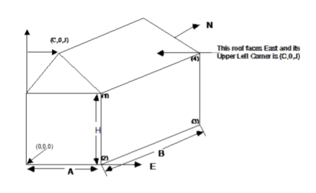
\includegraphics[width=0.9\textwidth, height=0.9\textheight, keepaspectratio=true]{media/image055.png}
\caption{Illustration for Surface Vertices \protect \label{fig:illustration-for-surface-vertices}}
\end{figure}

The figure above will help illustrate Surface Vertex entry. The convention used in ``GlobalGeometryRules'' dictates the order of the vertices (ref: GlobalGeometryRules). In this example, the conventions used are Starting Vertex Position = UpperLeftCorner and Vertex Entry Direction = CounterClockwise. The surfaces for this single zone are:

\begin{lstlisting}
4,0,0,H, 0,0,0, A,0,0, A,0,H; ! (4 vertices, South Wall)
4,A,0,H,A,0,0,A,B,0,A,B,H; ! (4 vertices, East Wall)
     ignore other walls that are not shown in this figure
4,C,0,J,A,0,H,A,B,H,C,B,J; ! (4 vertices, roof)
3,C,0,J,0,0,H,A,0,H; ! (3 vertices, gable end)
4,0,0,H, 0,0,0, A,0,0, A,0,H; ! (4 vertices, South Wall)
\end{lstlisting}

Note that in this example, point 1 of the entry is the Upper Left Corner of the rectangular surfaces and the point of the triangle for the 3 sided surface. The east wall shows the order of vertex entry. For horizontal surfaces, any vertex may be chosen as the starting position, but the Vertex Entry Direction convention must be followed. The surface details report (Output: Surfaces:List, Details;) is very useful for reviewing the accuracy of surface geometry inputs (ref: Surface Output Variables/Reports and Variable Dictionary Reports).

From the detailed vertices, EnergyPlus tries to determine the ``height'' and ``width'' of the surface. Obviously, this doesn't work well for \textgreater{}4 sided surfaces; for these, if the calculated height and width are not close to the gross area for the surface, the height and width shown will be the square root of the area (and thus a square).

\subsection{Building Surfaces - Detailed}\label{building-surfaces---detailed}

A building surface is necessary for all calculations. There must be at least one building surface per zone. You can use the detailed descriptions as shown below or the simpler, rectangular surface descriptions shown earlier.

\subsection{Wall:Detailed}\label{walldetailed}

The Wall:Detailed object is used to describe walls.

\subsubsection{Inputs}\label{inputs-20-007}

\paragraph{Field: Name}\label{field-name-16-010}

This is a unique name associated with each building surface. It is used in several other places as a reference (e.g.~as the base surface name for a Window or Door).

\paragraph{Field: Construction Name}\label{field-construction-name-16}

This is the name of the construction (ref: Construction object) used in the surface. Regardless of location in the building, the ``full'' construction (all layers) is used. For example, for an interior wall separating two zones, zone x would have the outside layer (e.g.~drywall) as the material that shows in zone y and then the layers to the inside layer -- the material that shows in zone x. For symmetric constructions, the same construction can be used in the surfaces described in both zones.

\paragraph{Field: Zone Name}\label{field-zone-name-10-000}

This is the zone name to which the surface belongs.

\paragraph{Field: Outside Boundary Condition}\label{field-outside-boundary-condition}

This value can be one of several things depending on the actual kind of surface.

\begin{enumerate}
  \item
    \textbf{Surface} -- if this surface is an internal surface, then this is the choice. The value will either be a surface in the base zone or a surface in another zone. The heat balance between two zones can be accurately simulated by specifying a surface in an adjacent zone. EnergyPlus will simulate a group of zones simultaneously and will include the heat transfer between zones. However, as this increases the complexity of the calculations, it is not necessary to specify the other zone unless the two zones will have a significant temperature difference. If the two zones will not be very different (temperature wise), then the surface should use itself as the outside environment or specify this field as \textbf{Adiabatic}. The surface name on the ``outside'' of this surface (adjacent to) is placed in the next field.
  \item
    \textbf{Adiabatic} -- an internal surface in the same Zone. This surface will not transfer heat out of the zone, but will still store heat in thermal mass. Only the inside face of the surface will exchange heat with the zone (i.e.~two adiabatic surfaces are required to model internal partitions where both sides of the surface are exchanging heat with the zone). The Outside Boundary Condition Object can be left blank.
  \item
    \textbf{Zone} -- this is similar to Surface but EnergyPlus will automatically create the required surface in the adjacent zone when this is entered for the surface. If there are windows or doors on the surface, EnergyPlus automatically creates appropriate sub-surfaces as well.
  \item
    \textbf{Outdoors} -- if this surface is exposed to outside temperature conditions, then this is the choice. See Sun Exposure and Wind Exposure below for further specifications on this kind of surface.
  \item
    \textbf{Foundation} - uses an alternative model (currently only the Kiva\textsuperscript{TM} model) to account for the multi-dimensional heat transfer of foundation surfaces. The Outside Boundary Condition Object will refer to the name of a Foundation:Kiva object (or be left blank to use the default foundation without extra insulation).
  \item
    \textbf{Ground} - The temperature on the outside of this surface will be the Site:GroundTemperature:Surface value for the month.
  \item
    \textbf{GroundFCfactorMethod} -- if this surface is exposed to the ground and using the \textbf{Construction:CfactorUndergroundWall}, then this is the choice. The temperature on the outside of this surface will be the Site:GroundTemperature:FcfactorMethod value for the month.
  \item
    \textbf{OtherSideCoefficients} -- if this surface has a custom, user specified temperature or other parameters (See SurfaceProperty:OtherSideCoefficients specification), then this is the choice. The outside boundary condition will be the name of the SurfaceProperty:OtherSideCoefficients specification.
  \item
    \textbf{OtherSideConditionsModel} -- if this surface has a specially-modeled multi-skin component, such as a transpired collector or vented photovoltaic panel, attached to the outside (See SurfaceProperty:OtherSideConditionsModel specification), then this the choice. The outside face environment will be the name of the SurfaceProperty:OtherSideConditionsModel specification.
  \item
    \textbf{GroundSlabPreprocessorAverage} -- uses the average results from the Slab preprocessor calculations.
  \item
    \textbf{GroundSlabPreprocessorCore} -- uses the core results from the Slab preprocessor calculations.
  \item
    \textbf{GroundSlabPreprocessorPerimeter} -- uses the perimeter results from the Slab preprocessor calculations.
  \item
    \textbf{GroundBasementPreprocessorAverageWall} -- uses the average wall results from the Basement preprocessor calculations.
  \item
    \textbf{GroundBasementPreprocessorAverageFloor} -- uses the average floor results from the Basement preprocessor calculations.
  \item
    \textbf{GroundBasementPreprocessorUpperWall} -- uses the upper wall results from the Basement preprocessor calculations.
  \item
    \textbf{GroundBasementPreprocessorLowerWall} -- uses the lower wall results from the Basement preprocessor calculations.
\end{enumerate}

\paragraph{Field: Outside Boundary Condition Object}\label{field-outside-boundary-condition-object-6}

If neither Surface, Zone, Foundation, OtherSideCoefficients, or OtherSideConditionsModel are specified for the Outside Boundary Condition (previous field), then this field should be left blank.

As stated above, if the Outside Boundary Condition is ``Surface'', then this field's value must be the surface name whose inside face temperature will be forced on the outside face of the base surface. This permits heat exchange between adjacent zones (interzone heat transfer) when multiple zones are simulated, but can also be used to simulate middle zone behavior without modeling the adjacent zones. This is done by specifying a surface within the zone. For example, a middle floor zone can be modeled by making the floor the Outside Boundary Condition Object for the ceiling, and the ceiling the Outside Boundary Condition Object for the floor.

If the Outside Boundary Condition is Zone, then this field should contain the zone name of the adjacent zone for the surface.

\begin{callout}
Note: Zones with interzone heat transfer are not adiabatic and the internal surfaces contribute to gains or losses. Adiabatic surfaces are modeled by specifying the base surface itself in this field. Also, for interzone heat transfer, both surfaces must be represented -- for example, if you want interzone heat transfer to an attic space, the ceiling in the lower zone must have a surface object with the outside face environment as the floor in the attic and, likewise, there must be a floor surface object in the attic that references the ceiling surface name in the lower zone.
\end{callout}

Equally, if the Outside Boundary Condition is ``OtherSideCoefficients'', then this field's value must be the SurfaceProperty:OtherSideCoefficients name. Or if the Outside Boundary Condition is ``OtherSideConditionsModel'' then this field's value must be the SurfaceProperty:OtherSideConditionsModel name.

\paragraph{Field: Sun Exposure}\label{field-sun-exposure-000}

If the surface is exposed to the sun, then ``SunExposed'' should be entered in this field. Otherwise, ``NoSun'' should be entered.

Note, a cantilevered floor could have ``Outdoors'' but ``NoSun'' exposure.

\paragraph{Field: Wind Exposure}\label{field-wind-exposure}

If the surface is exposed to the Wind, then ``WindExposed'' should be entered in this field. Otherwise, ``NoWind'' should be entered.

\begin{callout}
Note: When a surface is specified with ``NoWind'', this has several implications. Within the heat balance code, this surface will default to using the simple ASHRAE exterior convection coefficient correlation with a zero wind speed. In addition, since the ASHRAE simple method does not have a separate value for equivalent long wavelength radiation to the sky and ground, using ``NoWind'' also eliminates long wavelength radiant exchange from the exterior of the surface to both the sky and the ground. Thus, only simple convection takes place at the exterior face of a surface specified with ``NoWind''.
\end{callout}

\paragraph{Field: View Factor to Ground}\label{field-view-factor-to-ground}

The fraction of the ground plane (assumed horizontal) that is visible from a heat-transfer surface. It is used to calculate the diffuse solar radiation from the ground that is incident on the surface.

For example, if there are no obstructions, a vertical surface sees half of the ground plane and so View Factor to Ground = 0.5. A horizontal downward-facing surface sees the entire ground plane, so View Factor to Ground = 1.0. A horizontal upward-facing surface (horizontal roof) does not see the ground at all, so View Factor to Ground = 0.0.

Unused if reflections option in Solar Distribution field in Building object input unless a DaylightingDevice:Shelf or DaylightingDevice:Tubular has been specified.

If you do not use the reflections option in the Solar Distribution field in your Building object input, you are responsible for entering the View Factor to Ground for each heat-transfer surface. Typical values for a surface that is not shadowed are obtained by the simple equation:

View Factor to Ground = (1-cos(SurfTilt))/2

For example, this gives 0.5 for a wall of tilt 90°. If the tilt of the wall changes, then the View Factor to Ground must also change.

If you enter \textbf{autocalculate} in this field, EnergyPlus will automatically calculate the view factor to ground based on the tilt of the surface.

If \textbf{you do use the reflections option in the Solar Distribution field} in your Building object input, you do \textbf{not} have to enter View Factor to Ground values. In this case the program will automatically calculate the value to use for each exterior surface taking into account solar shadowing (including shadowing of the ground by the building) and reflections from obstructions (ref: Building, Field: Solar Distribution).

However, if you do use the reflections option AND you are modeling a DaylightingDevice:Shelf or DaylightingDevice:Tubular, then you still need to enter some values of View Factor to Ground. For DaylightingDevice:Shelf you need to enter View Factor to Ground for the window associated with the shelf. And for DaylightingDevice:Tubular you need to enter the View Factor to Ground for the FenestrationSurface:Detailed corresponding to the dome of the tubular device.

Note 1: The corresponding view factor to the sky for diffuse solar radiation is not a user input; it is calculated within EnergyPlus based on surface orientation, sky solar radiance distribution, and shadowing surfaces.

Note 2: The view factors to the sky and ground for thermal infrared (long-wave) radiation are not user inputs; they are calculated within EnergyPlus based on surface tilt and shadowing surfaces. Shadowing surfaces are considered to have the same emissivity and temperature as the ground, so they are lumped together with the ground in calculating the ground IR view factor.

\paragraph{Field: Number of Vertices}\label{field-number-of-vertices}

This field specifies the number of sides in the surface (number of X,Y,Z vertex groups). For further information, see the discussion on ``Surface Vertices'' above.

\subsection{RoofCeiling:Detailed}\label{roofceilingdetailed}

The RoofCeiling:Detailed object is used to describe walls.

\subsubsection{Inputs}\label{inputs-21-007}

\paragraph{Field: Name}\label{field-name-17-008}

This is a unique name associated with each building surface. It is used in several other places as a reference (e.g.~as the base surface name for a Window or Door).

\paragraph{Field: Construction Name}\label{field-construction-name-17}

This is the name of the construction (ref: Construction object) used in the surface. Regardless of location in the building, the ``full'' construction (all layers) is used. For example, for an interior wall separating two zones, zone x would have the outside layer (e.g.~drywall) as the material that shows in zone y and then the layers to the inside layer -- the material that shows in zone x. For symmetric constructions, the same construction can be used in the surfaces described in both zones.

\paragraph{Field: Zone Name}\label{field-zone-name-11-000}

This is the zone name to which the surface belongs.

\paragraph{Field: Outside Boundary Condition}\label{field-outside-boundary-condition-1}

This value can be one of several things depending on the actual kind of surface.

\begin{enumerate}
  \item
    \textbf{Surface} -- if this surface is an internal surface, then this is the choice. The value will either be a surface in the base zone or a surface in another zone. The heat balance between two zones can be accurately simulated by specifying a surface in an adjacent zone. EnergyPlus will simulate a group of zones simultaneously and will include the heat transfer between zones. However, as this increases the complexity of the calculations, it is not necessary to specify the other zone unless the two zones will have a significant temperature difference. If the two zones will not be very different (temperature wise), then the surface should use itself as the outside environment or specify this field as \textbf{Adiabatic}. The surface name on the ``outside'' of this surface (adjacent to) is placed in the next field.
  \item
    \textbf{Adiabatic} -- an internal surface in the same Zone. This surface will not transfer heat out of the zone, but will still store heat in thermal mass. Only the inside face of the surface will exchange heat with the zone (i.e.~two adiabatic surfaces are required to model internal partitions where both sides of the surface are exchanging heat with the zone). The Outside Boundary Condition Object can be left blank.
  \item
    \textbf{Zone} -- this is similar to Surface but EnergyPlus will automatically create the required surface in the adjacent zone when this is entered for the surface. If there are windows or doors on the surface, EnergyPlus automatically creates appropriate sub-surfaces as well.
  \item
    \textbf{Outdoors} -- if this surface is exposed to outside temperature conditions, then this is the choice. See Sun Exposure and Wind Exposure below for further specifications on this kind of surface.
  \item
    \textbf{Ground} -- The temperature on the outside of this surface will be the Ground Temperature.
  \item
    \textbf{OtherSideCoefficients} -- if this surface has a custom, user specified temperature or other parameters (See SurfaceProperty:OtherSideCoefficients specification), then this is the choice. The outside boundary condition will be the name of the SurfaceProperty:OtherSideCoefficients specification.
  \item
    \textbf{OtherSideConditionsModel} -- if this surface has a specially-modeled multi-skin component, such as a transpired collector or vented photovoltaic panel, attached to the outside (See SurfaceProperty:OtherSideConditionsModel specification), then this the choice. The outside face environment will be the name of the SurfaceProperty:OtherSideConditionsModel specification.
  \item
    \textbf{GroundSlabPreprocessorAverage} -- uses the average results from the Slab preprocessor calculations.
  \item
    \textbf{GroundSlabPreprocessorCore} -- uses the core results from the Slab preprocessor calculations.
  \item
    \textbf{GroundSlabPreprocessorPerimeter} -- uses the perimeter results from the Slab preprocessor calculations.
  \item
    \textbf{GroundBasementPreprocessorAverageWall} -- uses the average wall results from the Basement preprocessor calculations.
  \item
    \textbf{GroundBasementPreprocessorAverageFloor} -- uses the average floor results from the Basement preprocessor calculations.
  \item
    \textbf{GroundBasementPreprocessorUpperWall} -- uses the upper wall results from the Basement preprocessor calculations.
  \item
    \textbf{GroundBasementPreprocessorLowerWall} -- uses the lower wall results from the Basement preprocessor calculations.
\end{enumerate}

\paragraph{Field: Outside Boundary Condition Object}\label{field-outside-boundary-condition-object-7}

If neither Surface, Zone, Foundation, OtherSideCoefficients, or OtherSideConditionsModel are specified for the Outside Boundary Condition (previous field), then this field should be left blank.

As stated above, if the Outside Boundary Condition is ``Surface'', then this field's value must be the surface name whose inside face temperature will be forced on the outside face of the base surface. This permits heat exchange between adjacent zones (interzone heat transfer) when multiple zones are simulated, but can also be used to simulate middle zone behavior without modeling the adjacent zones. This is done by specifying a surface within the zone. For example, a middle floor zone can be modeled by making the floor the Outside Boundary Condition Object for the ceiling, and the ceiling the Outside Boundary Condition Object for the floor.

If the Outside Boundary Condition is Zone, then this field should contain the zone name of the adjacent zone for the surface.

\begin{callout}
Note: Zones with interzone heat transfer are not adiabatic and the internal surfaces contribute to gains or losses. Adiabatic surfaces are modeled by specifying the base surface itself in this field. Also, for interzone heat transfer, both surfaces must be represented -- for example, if you want interzone heat transfer to an attic space, the ceiling in the lower zone must have a surface object with the outside face environment as the floor in the attic and, likewise, there must be a floor surface object in the attic that references the ceiling surface name in the lower zone.
\end{callout}

Equally, if the Outside Boundary Condition is ``OtherSideCoefficients'', then this field's value must be the SurfaceProperty:OtherSideCoefficients name. Or if the Outside Boundary Condition is ``OtherSideConditionsModel'' then this field's value must be the SurfaceProperty:OtherSideConditionsModel name.

\paragraph{Field: Sun Exposure}\label{field-sun-exposure-1}

If the surface is exposed to the sun, then ``SunExposed'' should be entered in this field. Otherwise, ``NoSun'' should be entered.

Note, a cantilevered floor could have ``Outdoors'' but ``NoSun'' exposure.

\paragraph{Field: Wind Exposure}\label{field-wind-exposure-1}

If the surface is exposed to the Wind, then ``WindExposed'' should be entered in this field. Otherwise, ``NoWind'' should be entered.

\begin{callout}
Note: When a surface is specified with ``NoWind'', this has several implications. Within the heat balance code, this surface will default to using the simple ASHRAE exterior convection coefficient correlation with a zero wind speed. In addition, since the ASHRAE simple method does not have a separate value for equivalent long wavelength radiation to the sky and ground, using ``NoWind'' also eliminates long wavelength radiant exchange from the exterior of the surface to both the sky and the ground. Thus, only simple convection takes place at the exterior face of a surface specified with ``NoWind''.
\end{callout}

\paragraph{Field: View Factor to Ground}\label{field-view-factor-to-ground-1}

The fraction of the ground plane (assumed horizontal) that is visible from a heat-transfer surface. It is used to calculate the diffuse solar radiation from the ground that is incident on the surface.

For example, if there are no obstructions, a vertical surface sees half of the ground plane and so View Factor to Ground = 0.5. A horizontal downward-facing surface sees the entire ground plane, so View Factor to Ground = 1.0. A horizontal upward-facing surface (horizontal roof) does not see the ground at all, so View Factor to Ground = 0.0.

Unused if reflections option in Solar Distribution field in Building object input unless a DaylightingDevice:Shelf or DaylightingDevice:Tubular has been specified.

If you do not use the reflections option in the Solar Distribution field in your Building object input, you are responsible for entering the View Factor to Ground for each heat-transfer surface. Typical values for a surface that is not shadowed are obtained by the simple equation:

View Factor to Ground = (1-cos(SurfTilt))/2

For example, this gives 0.5 for a wall of tilt 90°. If the tilt of the wall changes, then the View Factor to Ground must also change.

If you enter \textbf{autocalculate} in this field, EnergyPlus will automatically calculate the view factor to ground based on the tilt of the surface.

If \textbf{you do use the reflections option in the Solar Distribution field} in your Building object input, you do \textbf{not} have to enter View Factor to Ground values. In this case the program will automatically calculate the value to use for each exterior surface taking into account solar shadowing (including shadowing of the ground by the building) and reflections from obstructions (ref: Building, Field: Solar Distribution).

However, if you do use the reflections option AND you are modeling a DaylightingDevice:Shelf or DaylightingDevice:Tubular, then you still need to enter some values of View Factor to Ground. For DaylightingDevice:Shelf you need to enter View Factor to Ground for the window associated with the shelf. And for DaylightingDevice:Tubular you need to enter the View Factor to Ground for the FenestrationSurface:Detailed corresponding to the dome of the tubular device.

Note 1: The corresponding view factor to the sky for diffuse solar radiation is not a user input; it is calculated within EnergyPlus based on surface orientation, sky solar radiance distribution, and shadowing surfaces.

Note 2: The view factors to the sky and ground for thermal infrared (long-wave) radiation are not user inputs; they are calculated within EnergyPlus based on surface tilt and shadowing surfaces. Shadowing surfaces are considered to have the same emissivity and temperature as the ground, so they are lumped together with the ground in calculating the ground IR view factor.

\paragraph{Field: Number of Vertices}\label{field-number-of-vertices-1}

This field specifies the number of sides in the surface (number of X,Y,Z vertex groups). For further information, see the discussion on ``Surface Vertices'' above.

\subsection{Floor:Detailed}\label{floordetailed}

The Floor:Detailed object is used to describe walls.

\subsubsection{Inputs}\label{inputs-22-006}

\paragraph{Field: Name}\label{field-name-18-008}

This is a unique name associated with each building surface. It is used in several other places as a reference (e.g.~as the base surface name for a Window or Door).

\paragraph{Field: Construction Name}\label{field-construction-name-18}

This is the name of the construction (ref: Construction object) used in the surface. Regardless of location in the building, the ``full'' construction (all layers) is used. For example, for an interior wall separating two zones, zone x would have the outside layer (e.g.~drywall) as the material that shows in zone y and then the layers to the inside layer -- the material that shows in zone x. For symmetric constructions, the same construction can be used in the surfaces described in both zones.

\paragraph{Field: Zone Name}\label{field-zone-name-12-000}

This is the zone name to which the surface belongs.

\paragraph{Field: Outside Boundary Condition}\label{field-outside-boundary-condition-2}

This value can be one of several things depending on the actual kind of surface.

\begin{enumerate}
  \item
    \textbf{Surface} -- if this surface is an internal surface, then this is the choice. The value will either be a surface in the base zone or a surface in another zone. The heat balance between two zones can be accurately simulated by specifying a surface in an adjacent zone. EnergyPlus will simulate a group of zones simultaneously and will include the heat transfer between zones. However, as this increases the complexity of the calculations, it is not necessary to specify the other zone unless the two zones will have a significant temperature difference. If the two zones will not be very different (temperature wise), then the surface should use itself as the outside environment or specify this field as \textbf{Adiabatic}. The surface name on the ``outside'' of this surface (adjacent to) is placed in the next field.
  \item
    \textbf{Adiabatic} -- an internal surface in the same Zone. This surface will not transfer heat out of the zone, but will still store heat in thermal mass. Only the inside face of the surface will exchange heat with the zone (i.e.~two adiabatic surfaces are required to model internal partitions where both sides of the surface are exchanging heat with the zone). The Outside Boundary Condition Object can be left blank.
  \item
    \textbf{Zone} -- this is similar to Surface but EnergyPlus will automatically create the required surface in the adjacent zone when this is entered for the surface. If there are windows or doors on the surface, EnergyPlus automatically creates appropriate sub-surfaces as well.
  \item
    \textbf{Outdoors} -- if this surface is exposed to outside temperature conditions, then this is the choice. See Sun Exposure and Wind Exposure below for further specifications on this kind of surface.
  \item
    \textbf{Foundation} - uses an alternative model (currently only the Kiva\textsuperscript{TM} model) to account for the multi-dimensional heat transfer of foundation surfaces. The Outside Boundary Condition Object will refer to the name of a Foundation:Kiva object (or be left blank to use the default foundation without extra insulation).
  \item
    \textbf{Ground} - The temperature on the outside of this surface will be the Site:GroundTemperature:Surface value for the month..
  \item
    \textbf{GroundFCfactorMethod} -- if this surface is exposed to the ground and using the \textbf{Construction:CfactorUndergroundWall}, then this is the choice. The temperature on the outside of this surface will be the Site:GroundTemperature:FcfactorMethod value for the month.
  \item
    \textbf{OtherSideCoefficients} -- if this surface has a custom, user specified temperature or other parameters (See SurfaceProperty:OtherSideCoefficients specification), then this is the choice. The outside boundary condition will be the name of the SurfaceProperty:OtherSideCoefficients specification.
  \item
    \textbf{OtherSideConditionsModel} -- if this surface has a specially-modeled multi-skin component, such as a transpired collector or vented photovoltaic panel, attached to the outside (See SurfaceProperty:OtherSideConditionsModel specification), then this the choice. The outside face environment will be the name of the SurfaceProperty:OtherSideConditionsModel specification.
  \item
    \textbf{GroundSlabPreprocessorAverage} -- uses the average results from the Slab preprocessor calculations.
  \item
    \textbf{GroundSlabPreprocessorCore} -- uses the core results from the Slab preprocessor calculations.
  \item
    \textbf{GroundSlabPreprocessorPerimeter} -- uses the perimeter results from the Slab preprocessor calculations.
  \item
    \textbf{GroundBasementPreprocessorAverageWall} -- uses the average wall results from the Basement preprocessor calculations.
  \item
    \textbf{GroundBasementPreprocessorAverageFloor} -- uses the average floor results from the Basement preprocessor calculations.
  \item
    \textbf{GroundBasementPreprocessorUpperWall} -- uses the upper wall results from the Basement preprocessor calculations.
  \item
    \textbf{GroundBasementPreprocessorLowerWall} -- uses the lower wall results from the Basement preprocessor calculations.
\end{enumerate}

\paragraph{Field: Outside Boundary Condition Object}\label{field-outside-boundary-condition-object-8}

If neither Surface, Zone, Foundation, OtherSideCoefficients, or OtherSideConditionsModel are specified for the Outside Boundary Condition (previous field), then this field should be left blank.

As stated above, if the Outside Boundary Condition is ``Surface'', then this field's value must be the surface name whose inside face temperature will be forced on the outside face of the base surface. This permits heat exchange between adjacent zones (interzone heat transfer) when multiple zones are simulated, but can also be used to simulate middle zone behavior without modeling the adjacent zones. This is done by specifying a surface within the zone. For example, a middle floor zone can be modeled by making the floor the Outside Boundary Condition Object for the ceiling, and the ceiling the Outside Boundary Condition Object for the floor.

If the Outside Boundary Condition is Zone, then this field should contain the zone name of the adjacent zone for the surface.

\begin{callout}
Note: Zones with interzone heat transfer are not adiabatic and the internal surfaces contribute to gains or losses. Adiabatic surfaces are modeled by specifying the base surface itself in this field. Also, for interzone heat transfer, both surfaces must be represented -- for example, if you want interzone heat transfer to an attic space, the ceiling in the lower zone must have a surface object with the outside face environment as the floor in the attic and, likewise, there must be a floor surface object in the attic that references the ceiling surface name in the lower zone.
\end{callout}

Equally, if the Outside Boundary Condition is ``OtherSideCoefficients'', then this field's value must be the SurfaceProperty:OtherSideCoefficients name. Or if the Outside Boundary Condition is ``OtherSideConditionsModel'' then this field's value must be the SurfaceProperty:OtherSideConditionsModel name.

\paragraph{Field: Sun Exposure}\label{field-sun-exposure-2}

If the surface is exposed to the sun, then ``SunExposed'' should be entered in this field. Otherwise, ``NoSun'' should be entered.

Note, a cantilevered floor could have ``Outdoors'' but ``NoSun'' exposure.

\paragraph{Field: Wind Exposure}\label{field-wind-exposure-2}

If the surface is exposed to the Wind, then ``WindExposed'' should be entered in this field. Otherwise, ``NoWind'' should be entered.

\begin{callout}
Note: When a surface is specified with ``NoWind'', this has several implications. Within the heat balance code, this surface will default to using the simple ASHRAE exterior convection coefficient correlation with a zero wind speed. In addition, since the ASHRAE simple method does not have a separate value for equivalent long wavelength radiation to the sky and ground, using ``NoWind'' also eliminates long wavelength radiant exchange from the exterior of the surface to both the sky and the ground. Thus, only simple convection takes place at the exterior face of a surface specified with ``NoWind''.
\end{callout}

\paragraph{Field: View Factor to Ground}\label{field-view-factor-to-ground-2}

The fraction of the ground plane (assumed horizontal) that is visible from a heat-transfer surface. It is used to calculate the diffuse solar radiation from the ground that is incident on the surface.

For example, if there are no obstructions, a vertical surface sees half of the ground plane and so View Factor to Ground = 0.5. A horizontal downward-facing surface sees the entire ground plane, so View Factor to Ground = 1.0. A horizontal upward-facing surface (horizontal roof) does not see the ground at all, so View Factor to Ground = 0.0.

Unused if reflections option in Solar Distribution field in Building object input unless a DaylightingDevice:Shelf or DaylightingDevice:Tubular has been specified.

If you do not use the reflections option in the Solar Distribution field in your Building object input, you are responsible for entering the View Factor to Ground for each heat-transfer surface. Typical values for a surface that is not shadowed are obtained by the simple equation:

View Factor to Ground = (1-cos(SurfTilt))/2

For example, this gives 0.5 for a wall of tilt 90°. If the tilt of the wall changes, then the View Factor to Ground must also change.

If you enter \textbf{autocalculate} in this field, EnergyPlus will automatically calculate the view factor to ground based on the tilt of the surface.

If \textbf{you do use the reflections option in the Solar Distribution field} in your Building object input, you do \textbf{not} have to enter View Factor to Ground values. In this case the program will automatically calculate the value to use for each exterior surface taking into account solar shadowing (including shadowing of the ground by the building) and reflections from obstructions (ref: Building, Field: Solar Distribution).

However, if you do use the reflections option AND you are modeling a DaylightingDevice:Shelf or DaylightingDevice:Tubular, then you still need to enter some values of View Factor to Ground. For DaylightingDevice:Shelf you need to enter View Factor to Ground for the window associated with the shelf. And for DaylightingDevice:Tubular you need to enter the View Factor to Ground for the FenestrationSurface:Detailed corresponding to the dome of the tubular device.

Note 1: The corresponding view factor to the sky for diffuse solar radiation is not a user input; it is calculated within EnergyPlus based on surface orientation, sky solar radiance distribution, and shadowing surfaces.

Note 2: The view factors to the sky and ground for thermal infrared (long-wave) radiation are not user inputs; they are calculated within EnergyPlus based on surface tilt and shadowing surfaces. Shadowing surfaces are considered to have the same emissivity and temperature as the ground, so they are lumped together with the ground in calculating the ground IR view factor.

\paragraph{Field: Number of Vertices}\label{field-number-of-vertices-2}

This field specifies the number of sides in the surface (number of X,Y,Z vertex groups). For further information, see the discussion on ``Surface Vertices'' above.

Some examples of using these objects:

\begin{lstlisting}

Floor:Detailed,
      Floor_NorthZone_1stFloor,!- Name
      FLOOR-SLAB-ASSEMBLY,     !- Construction Name
      NorthZone_1stFloor,      !- Zone Name
      Ground,                  !- Outside Boundary Condition
      ,                        !- Outside Boundary Condition Object
      NoSun,                   !- Sun Exposure
      NoWind,                  !- Wind Exposure
      0.0,                     !- View Factor to Ground
      4,                       !- Number of Vertices
      0, 11, 0,                           !- X,Y,Z  1 {m}
      25, 11, 0,                          !- X,Y,Z  2 {m}
      25, 5.5, 0,                         !- X,Y,Z  3 {m}
     0, 5.5, 0;                          !- X,Y,Z  4 {m}

  RoofCeiling:Detailed,
      Ceiling_SouthZone_1stFloor,  !- Name
      CEILING-FLOOR-ASSEMBLY,  !- Construction Name
      SouthZone_1stFloor,      !- Zone Name
      Surface,                 !- Outside Boundary Condition
      Floor_SouthZone_2ndFloor,!- Outside Boundary Condition Object
      NoSun,                   !- Sun Exposure
      NoWind,                  !- Wind Exposure
      0.0,                     !- View Factor to Ground
      4,                       !- Number of Vertices
      0, 0, 3.4,                          !- X,Y,Z  1 {m}
      25, 0, 3.4,                         !- X,Y,Z  2 {m}
      25, 5.5, 3.4,                       !- X,Y,Z  3 {m}
     0, 5.5, 3.4;                        !- X,Y,Z  4 {m}

  Wall:Detailed,
      InteriorWall_SouthZone_1stFloor,  !- Name
      INTERIOR-WALL-ASSEMBLY,  !- Construction Name
      SouthZone_1stFloor,      !- Zone Name
      Surface,                 !- Outside Boundary Condition
      InteriorWall_NorthZone_1stFloor,  !- Outside Boundary Condition Object
      NoSun,                   !- Sun Exposure
      NoWind,                  !- Wind Exposure
      0,                       !- View Factor to Ground
      4,                       !- Number of Vertices
      25, 5.5, 3.7,                       !- X,Y,Z  1 {m}
      25, 5.5, 0,                         !- X,Y,Z  2 {m}
      0, 5.5, 0,                          !- X,Y,Z  3 {m}
     0, 5.5, 3.7;                        !- X,Y,Z  4 {m}
\end{lstlisting}

\subsection{BuildingSurface:Detailed}\label{buildingsurfacedetailed}

The BuildingSurface:Detailed object can more generally describe each of the surfaces.

\subsubsection{Inputs}\label{inputs-23-006}

\paragraph{Field: Name}\label{field-name-19-005}

This is a unique name associated with each building surface. It is used in several other places as a reference (e.g.~as the base surface name for a Window or Door).

\paragraph{Field: Surface Type}\label{field-surface-type-000}

Used primarily for convenience, the surface type can be one of the choices illustrated above -- Wall, Floor, Ceiling, Roof. Azimuth (facing) and Tilt are determined from the vertex coordinates. Note that ``normal'' floors will be tilted 180° whereas flat roofs/ceilings will be tilted 0°. EnergyPlus uses this field's designation, along with the calculated tilt of the surface, to issue warning messages when tilts are ``out of range''. Calculations in EnergyPlus use the actual calculated tilt values for the actual heat balance calculations. Note, however, that a floor tilted 0° is really facing ``into'' the zone and is not what you will desire for the calculations even though the coordinate may appear correct in the viewed DXF display.

``Normal'' tilt for walls is 90° -- here you may use the calculated Azimuth to make sure your walls are facing away from the zone's interior.

\paragraph{Field: Construction Name}\label{field-construction-name-19}

This is the name of the construction (ref: Construction object) used in the surface. Regardless of location in the building, the ``full'' construction (all layers) is used. For example, for an interior wall separating two zones, zone x would have the outside layer (e.g.~drywall) as the material that shows in zone y and then the layers to the inside layer -- the material that shows in zone x. For symmetric constructions, the same construction can be used in the surfaces described in both zones.

\paragraph{Field: Zone Name}\label{field-zone-name-13}

This is the zone name to which the surface belongs.

\paragraph{Field: Outside Boundary Condition}\label{field-outside-boundary-condition-3}

This value can be one of several things depending on the actual kind of surface.

\begin{enumerate}
  \item
    \textbf{Surface} -- if this surface is an internal surface, then this is the choice. The value will either be a surface in the base zone or a surface in another zone. The heat balance between two zones can be accurately simulated by specifying a surface in an adjacent zone. EnergyPlus will simulate a group of zones simultaneously and will include the heat transfer between zones. However, as this increases the complexity of the calculations, it is not necessary to specify the other zone unless the two zones will have a significant temperature difference. If the two zones will not be very different (temperature wise), then the surface should use itself as the outside environment or specify this field as \textbf{Adiabatic}. The surface name on the ``outside'' of this surface (adjacent to) is placed in the next field.
  \item
    \textbf{Adiabatic} -- an internal surface in the same Zone. This surface will not transfer heat out of the zone, but will still store heat in thermal mass. Only the inside face of the surface will exchange heat with the zone (i.e.~two adiabatic surfaces are required to model internal partitions where both sides of the surface are exchanging heat with the zone). The Outside Boundary Condition Object can be left blank.
  \item
    \textbf{Zone} -- this is similar to Surface but EnergyPlus will automatically create the required surface in the adjacent zone when this is entered for the surface. If there are windows or doors on the surface, EnergyPlus automatically creates appropriate sub-surfaces as well.
  \item
    \textbf{Outdoors} -- if this surface is exposed to outside temperature conditions, then this is the choice. See Sun Exposure and Wind Exposure below for further specifications on this kind of surface.
  \item
    \textbf{Foundation} - uses an alternative model (currently only the Kiva\textsuperscript{TM} model) to account for the multi-dimensional heat transfer of foundation surfaces. The Outside Boundary Condition Object will refer to the name of a Foundation:Kiva object (or be left blank to use the default foundation without extra insulation).
  \item
    \textbf{Ground} - The temperature on the outside of this surface will be the Site:GroundTemperature:Surface value for the month.
  \item
    \textbf{GroundFCfactorMethod} -- if this surface is exposed to the ground and using the \textbf{Construction:CfactorUndergroundWall}, then this is the choice. The temperature on the outside of this surface will be the Site:GroundTemperature:FcfactorMethod value for the month.
  \item
    \textbf{OtherSideCoefficients} -- if this surface has a custom, user specified temperature or other parameters (See SurfaceProperty:OtherSideCoefficients specification), then this is the choice. The outside boundary condition will be the name of the SurfaceProperty:OtherSideCoefficients specification.
  \item
    \textbf{OtherSideConditionsModel} -- if this surface has a specially-modeled multi-skin component, such as a transpired collector or vented photovoltaic panel, attached to the outside (See SurfaceProperty:OtherSideConditionsModel specification), then this the choice. The outside face environment will be the name of the SurfaceProperty:OtherSideConditionsModel specification.
  \item
    \textbf{GroundSlabPreprocessorAverage} -- uses the average results from the Slab preprocessor calculations.
  \item
    \textbf{GroundSlabPreprocessorCore} -- uses the core results from the Slab preprocessor calculations.
  \item
    \textbf{GroundSlabPreprocessorPerimeter} -- uses the perimeter results from the Slab preprocessor calculations.
  \item
    \textbf{GroundBasementPreprocessorAverageWall} -- uses the average wall results from the Basement preprocessor calculations.
  \item
    \textbf{GroundBasementPreprocessorAverageFloor} -- uses the average floor results from the Basement preprocessor calculations.
  \item
    \textbf{GroundBasementPreprocessorUpperWall} -- uses the upper wall results from the Basement preprocessor calculations.
  \item
    \textbf{GroundBasementPreprocessorLowerWall} -- uses the lower wall results from the Basement preprocessor calculations.
\end{enumerate}

\paragraph{Field: Outside Boundary Condition Object}\label{field-outside-boundary-condition-object-9}

If neither Surface, Zone, Foundation, OtherSideCoefficients, or OtherSideConditionsModel are specified for the Outside Boundary Condition (previous field), then this field should be left blank.

As stated above, if the Outside Boundary Condition is ``Surface'', then this field's value must be the surface name whose inside face temperature will be forced on the outside face of the base surface. This permits heat exchange between adjacent zones (interzone heat transfer) when multiple zones are simulated, but can also be used to simulate middle zone behavior without modeling the adjacent zones. This is done by specifying a surface within the zone. For example, a middle floor zone can be modeled by making the floor the Outside Boundary Condition Object for the ceiling, and the ceiling the Outside Boundary Condition Object for the floor.

If the Outside Boundary Condition is Zone, then this field should contain the zone name of the adjacent zone for the surface.

\begin{callout}
Note: Zones with interzone heat transfer are not adiabatic and the internal surfaces contribute to gains or losses. Adiabatic surfaces are modeled by specifying the base surface itself in this field. Also, for interzone heat transfer, both surfaces must be represented -- for example, if you want interzone heat transfer to an attic space, the ceiling in the lower zone must have a surface object with the outside face environment as the floor in the attic and, likewise, there must be a floor surface object in the attic that references the ceiling surface name in the lower zone.
\end{callout}

Equally, if the Outside Boundary Condition is ``OtherSideCoefficients'', then this field's value must be the SurfaceProperty:OtherSideCoefficients name. Or if the Outside Boundary Condition is ``OtherSideConditionsModel'' then this field's value must be the SurfaceProperty:OtherSideConditionsModel name.

\paragraph{Field: Sun Exposure}\label{field-sun-exposure-3}

If the surface is exposed to the sun, then ``SunExposed'' should be entered in this field. Otherwise, ``NoSun'' should be entered.

Note, a cantilevered floor could have ``Outdoors'' but ``NoSun'' exposure.

\paragraph{Field: Wind Exposure}\label{field-wind-exposure-3}

If the surface is exposed to the Wind, then ``WindExposed'' should be entered in this field. Otherwise, ``NoWind'' should be entered.

\begin{callout}
Note: When a surface is specified with ``NoWind'', this has several implications. Within the heat balance code, this surface will default to using the simple ASHRAE exterior convection coefficient correlation with a zero wind speed. In addition, since the ASHRAE simple method does not have a separate value for equivalent long wavelength radiation to the sky and ground, using ``NoWind'' also eliminates long wavelength radiant exchange from the exterior of the surface to both the sky and the ground. Thus, only simple convection takes place at the exterior face of a surface specified with ``NoWind''.
\end{callout}

\paragraph{Field: View Factor to Ground}\label{field-view-factor-to-ground-3}

The fraction of the ground plane (assumed horizontal) that is visible from a heat-transfer surface. It is used to calculate the diffuse solar radiation from the ground that is incident on the surface.

For example, if there are no obstructions, a vertical surface sees half of the ground plane and so View Factor to Ground = 0.5. A horizontal downward-facing surface sees the entire ground plane, so View Factor to Ground = 1.0. A horizontal upward-facing surface (horizontal roof) does not see the ground at all, so View Factor to Ground = 0.0.

Unused if reflections option in Solar Distribution field in Building object input unless a DaylightingDevice:Shelf or DaylightingDevice:Tubular has been specified.

If you do not use the reflections option in the Solar Distribution field in your Building object input, you are responsible for entering the View Factor to Ground for each heat-transfer surface. Typical values for a surface that is not shadowed are obtained by the simple equation:

View Factor to Ground = (1-cos(SurfTilt))/2

For example, this gives 0.5 for a wall of tilt 90°. If the tilt of the wall changes, then the View Factor to Ground must also change.

If you enter \textbf{autocalculate} in this field, EnergyPlus will automatically calculate the view factor to ground based on the tilt of the surface.

If \textbf{you do use the reflections option in the Solar Distribution field} in your Building object input, you do \textbf{not} have to enter View Factor to Ground values. In this case the program will automatically calculate the value to use for each exterior surface taking into account solar shadowing (including shadowing of the ground by the building) and reflections from obstructions (ref: Building, Field: Solar Distribution).

However, if you do use the reflections option AND you are modeling a DaylightingDevice:Shelf or DaylightingDevice:Tubular, then you still need to enter some values of View Factor to Ground. For DaylightingDevice:Shelf you need to enter View Factor to Ground for the window associated with the shelf. And for DaylightingDevice:Tubular you need to enter the View Factor to Ground for the FenestrationSurface:Detailed corresponding to the dome of the tubular device.

Note 1: The corresponding view factor to the sky for diffuse solar radiation is not a user input; it is calculated within EnergyPlus based on surface orientation, sky solar radiance distribution, and shadowing surfaces.

Note 2: The view factors to the sky and ground for thermal infrared (long-wave) radiation are not user inputs; they are calculated within EnergyPlus based on surface tilt and shadowing surfaces. Shadowing surfaces are considered to have the same emissivity and temperature as the ground, so they are lumped together with the ground in calculating the ground IR view factor.

\paragraph{Field: Number of Vertices}\label{field-number-of-vertices-3}

This field specifies the number of sides in the surface (number of X,Y,Z vertex groups). For further information, see the discussion on ``Surface Vertices'' above.

IDF example of three walls (first is an exterior wall, second and third are interzone partitions):

\begin{lstlisting}

BuildingSurface:Detailed,Zn001:Wall001,  !- Base Surface Name
    Wall,EXTERIOR,  !- Class and Construction Name
    ZONE 1 @ 200 601 0 T,  !- Zone
    Outdoors,,  !- Outside Boundary Condition  and Target (if applicable)
     SunExposed,  !- Solar Exposure
     WindExposed,  !- Wind Exposure
    0.5000000    ,  !- VF to Ground
             4, !-Rectangle
    0.0000000E+00,  0.0000000E+00,   3.048000    ,
    0.0000000E+00,  0.0000000E+00,  0.0000000E+00,
     6.096000    ,  0.0000000E+00,  0.0000000E+00,
     6.096000    ,  0.0000000E+00,   3.048000    ;

  BuildingSurface:Detailed,Zn001:Wall006,  !-Base Surface Name
    Wall,INTERIOR,  !- Class and Construction Name
    HEARTLAND AREA,  !- Zone
    Surface,Zn004:Wall005,  !- Outside Boundary Conditions and Target (if applicable)
     NoSun,  !- Solar Exposure
     NoWind,  !- Wind Exposure
    0.5000000    ,  !- VF to Ground
             4, !-Rectangle
     38.01000    ,   28.25000    ,   10.00000    ,
     38.01000    ,   28.25000    ,  0.0000000E+00,
     38.01000    ,   18.25000    ,  0.0000000E+00,
     38.01000    ,   18.25000    ,   10.00000    ;

  BuildingSurface:Detailed,Zn001:Wall007,  !- Base Surface Name
    Wall,INTERIOR,  !- Class and Construction Name
    HEARTLAND AREA,  !- Zone
    Surface,Zn003:Wall006,  !- Outside Boundary Conditions and Target (if applicable)
     NoSun,  !- Solar Exposure
     NoWind,  !- Wind Exposure
    0.5000000    ,  !- VF to Ground
             4, !-Rectangle
     58.01000    ,   18.25000    ,   10.00000    ,
     58.01000    ,   18.25000    ,  0.0000000E+00,
     58.01000    ,   28.25000    ,  0.0000000E+00,
     58.01000    ,   28.25000    ,   10.00000    ;
\end{lstlisting}

\subsection{FenestrationSurface:Detailed}\label{fenestrationsurfacedetailed}

This surface class is used for subsurfaces, which can be of five different types: Windows, Doors, GlassDoors, TubularDaylightDomes, and TubularDaylightDiffusers. A subsurface (such as a window) of a base surface (such as a wall) inherits several of the properties (such as Outside Boundary Condition, Sun Exposure, etc.) of the base surface. Windows, GlassDoors, TubularDaylightDomes, and TubularDaylightDiffusers are considered to have one or more glass layers and so transmit solar radiation. Doors are considered to be opaque. For Surface Type = Window and GlassDoor, shades and screens may be applied by referencing this subsurface in a window shading control (ref: WindowShadingControl object). To assign a shade to a window or glass door, see WindowMaterial: Shade. To assign a screen, see WindowMaterial:Screen. To assign a blind, see WindowMaterial:Blind. To assign switchable glazing, such as electrochromic glazing, see WindowShadingControl.

The surface can be of 3 sides or 4 sides. A 4-sided but non-rectangular fenestration surface is allowed and will be transferred to an equivalent rectangular surface with the same area and aspect ratio for the convection calculations at window air gaps.

\subsubsection{Inputs}\label{inputs-24-004}

\paragraph{Field: Name}\label{field-name-20-004}

This is a unique name associated with the heat transfer subsurface. It may be used in other places as a reference (e.g.~as the opposing subsurface of an interzone window or door).

\paragraph{Field: Surface Type}\label{field-surface-type-2016-06-16}

The choices for Surface Type are Window, Door, GlassDoor, TubularDaylightDome, and TubularDaylightDiffuser. Doors are assumed to be opaque (do not transmit solar radiation) whereas the other surface types do transmit solar radiation. Windows and Glass Doors are treated identically in the calculation of conduction heat transfer, solar gain, daylighting, etc. A Window or GlassDoor, but not a Door, can have a movable interior, exterior or between-glass shading device, such as blinds (ref: WindowMaterial:Blind object), and can have a frame and/or a divider (ref: WindowProperty:FrameAndDivider object). TubularDaylightDomes and TubularDaylightDomes are specialized subsurfaces for use with the DaylightingDevice:Tubular object to simulate Tubular Daylighting Devices (TDDs). TubularDaylightDomes and TubularDaylightDomes cannot have shades, screens or blinds. In the following, the term ``window'' applies to Window, GlassDoor, TubularDaylightDome, and TubularDaylightDome, if not otherwise explicitly mentioned.

As noted in the description of the BuildingSurface:Detailed, Azimuth (facing angle) and Tilt are calculated from the entered vertices. Tilts of subsurfaces will normally be the same as their base surface. If these are significantly beyond the ``normals'' for the base surface, warning messages may be issued. If the facing angles are not correct, you may have a window pointing ``into'' the zone rather than out of it -- this would cause problems in the calculations. Note, too, that a ``reveal'' (inset or outset) may occur if the plane of the subsurface is not coincident with the base surface; the reveal has an effect on shading of the subsurface.

\paragraph{Field: Construction Name}\label{field-construction-name-20}

This is the name of the subsurface's construction (ref: Construction object {[}for Door{]} and Construction, Construction:ComplexFenestrationState, Construction:WindowDataFile objects {[}for Window and GlassDoor{]}).

For windows, if Construction Name is not found among the constructions on the input (.idf) file, the Window Data File (ref. Construction:WindowDataFile object) will be searched for that Construction Name (see ``Importing Windows from WINDOW''). If that file is not present or if the Construction Name does not match the name of an entry on the file, an error will result. If there is a match, a window construction and its corresponding glass and gas materials will be created from the information read from the file.

\paragraph{Field: Building Surface Name}\label{field-building-surface-name-6}

This is the name of a surface that contains this subsurface. Certain kinds of surfaces may not be allowed to have subsurfaces. For example, a surface in contact with the ground (Outside Boundary Condition = Ground) cannot contain a window.

\paragraph{Field: Outside Boundary Condition Object}\label{field-outside-boundary-condition-object-10}

If the base surface has Outside Boundary Condition = Surface or OtherSideCoefficients, then this field must also be specified for the subsurface. Otherwise, it can be left blank.

If the base surface has Outside Boundary Condition = Zone, then this surface retains that characteristic and uses the same zone of the base surface. It can be entered here for clarity or it can be left blank.

If Outside Boundary Condition for the base surface is Surface, this field should specify the subsurface in the opposing zone that is the counterpart to this subsurface. The constructions of the subsurface and opposing subsurface must match, except that, for multi-layer constructions, the layer order of the opposing subsurface's construction must be the reverse of that of the subsurface.

If Outside Boundary Condition for the base surface is OtherSideCoefficients, this field could specify the set of SurfaceProperty:OtherSideCoefficients for this subsurface. If this is left blank, then the Other Side Coefficients of the base surface will be used for this subsurface. \emph{Windows and GlassDoors are not allowed to have Other Side Coefficients.}

\paragraph{Field: View Factor to Ground}\label{field-view-factor-to-ground-4}

The fraction of the ground plane (assumed horizontal) that is visible from a heat-transfer surface. It is used to calculate the diffuse solar radiation from the ground that is incident on the surface.

For example, if there are no obstructions, a vertical surface sees half of the ground plane and so View Factor to Ground = 0.5. A horizontal downward-facing surface sees the entire ground plane, so View Factor to Ground = 1.0. A horizontal upward-facing surface (horizontal roof) does not see the ground at all, so View Factor to Ground = 0.0.

Unused if reflections option in Solar Distribution field in Building object input unless a Daylighting Device:Shelf or Daylighting Device:Tubular has been specified.

If you do not use the reflections option in the Solar Distribution field in your Building object input, you are responsible for entering the View Factor to Ground for each heat-transfer surface. Typical values for a surface that is not shadowed are obtained by the simple equation:

View Factor to Ground = (1-cos(SurfTilt))/2

For example, this gives 0.5 for a wall of tilt 90°. If the tilt of the wall changes, then the View Factor to Ground must also change.

If you enter \textbf{autocalculate} in this field, EnergyPlus will automatically calculate the view factor to ground based on the tilt of the surface.

If \textbf{you do use the reflections option in the Solar Distribution field} in your BUILDING object input, you do \textbf{not} have to enter View Factor to Ground values. In this case the program will automatically calculate the value to use for each exterior surface taking into account solar shadowing (including shadowing of the ground by the building) and reflections from obstructions (ref: Building, Field: Solar Distribution).

However, if you do use the reflections option AND you are modeling a DaylightingDevice:Shelf or DaylightingDevice:Tubular, then you still need to enter some values of View Factor to Ground. For DaylightingDevice:Shelf you need to enter View Factor to Ground for the window associated with the shelf. And for DaylightingDevice:Tubular you need to enter the View Factor to Ground for the FenestrationSurface:Detailed corresponding to the dome of the tubular device (ref: DaylightingDevice:Tubular).

Note 1: The corresponding view factor to the sky for diffuse solar radiation is not a user input; it is calculated within EnergyPlus based on surface orientation, sky solar radiance distribution, and shadowing surfaces.

Note 2: The view factors to the sky and ground for thermal infrared (long-wave) radiation are not user inputs; they are calculated within EnergyPlus based on surface tilt and shadowing surfaces. Shadowing surfaces are considered to have the same emissivity and temperature as the ground, so they are lumped together with the ground in calculating the ground infrared view factor.

\paragraph{Field: Frame and Divider Name}\label{field-frame-and-divider-name-2}

This field, if not blank, can be used to specify window frame, divider and reveal-surface data (ref: WindowProperty:FrameAndDivider object). It is used only for exterior GlassDoors and rectangular exterior Windows, i.e., those with OutsideFaceEnvironment = Outdoors.

This field should be blank for triangular windows.

\paragraph{Field: Multiplier}\label{field-multiplier-7}

Used only for Surface Type = Window, Door or Glass Door. It is the number of identical items on the base surface. Using Multiplier can save input effort and calculation time. In the calculation the area (and area of frame and divider, if present and surface type is a window) is multiplied by Multiplier. The calculation of shadowing on the subsurfaces (and the calculation of the interior distribution of beam solar radiation transmitted by windows and glass doors) are done for the specified subsurface position and dimensions.

Multiplier should be used with caution. Multiplier \textgreater{} 1 can give inaccurate or nonsensical results in situations where the results are sensitive to window or glass door position. This includes shadowing on the window/glass door, daylighting from the window/glass door, and interior distribution of solar radiation from the window/glass door. In these cases, the results for the single input window/glass door, after multiplication, may not be representative of the results you would get if you entered each of the multiple subsurfaces separately.

If Multiplier \textgreater{} 1, you will get

--a \emph{warning} if Solar Distribution = FullExterior or FullInteriorAndExterior (ref: Building - Field: Solar Distribution), indicating that the shadowing on the input window or the interior solar radiation distribution from the input window may not be representative of the actual group of windows. No warning is issued if Solar Distribution = MinimalShadowing.

--an \emph{error} if the window is an exterior window/glass door in a zone that has a detailed daylighting calculation (Daylighting:Detailed specified for the zone). Since a single window with a multiplier can never give the same daylight illuminance as the actual set of windows, you are not allowed to use Multiplier in this situation.

\paragraph{Field: Number of Vertices}\label{field-number-of-vertices-4}

The number of sides the surface has (number of X,Y,Z vertex groups). For further information, see the discussion on ``Surface Vertices'' above. Door and GlassDoor subsurfaces are rectangular and therefore have four vertices. Window subsurfaces can be rectangular or triangular and therefore have four or three vertices, respectively.

\paragraph{Fields: Vertex Coordinates}\label{fields-vertex-coordinates}

This is a total of twelve fields giving the x,y,z coordinate values of the four vertices of rectangular subsurfaces {[}m{]}, or a total of nine fields giving the x,y,z coordinate values of the three vertices of triangular windows.

For triangular windows the first vertex listed can be any of the three vertices, but the order of the vertices should be counter-clockwise if VertexEntry is CounterClockWise and clockwise if VertexEntry is ClockWise (ref: GlobalGeometryRules).

An IDF example of a rectangular subsurface (Window):

\begin{lstlisting}

FenestrationSurface:Detailed,
   Zn001:Wall001:Win001,  !- SubSurface Name
    Window,SINGLE PANE HW WINDOW,  !- Class and Construction Name
    Zn001:Wall001,,         !- Base Surface Name and Target (if applicable)
    0.5000000    ,          !- VF to Ground
    WINDOW-CONTROL-DRAPES,  !- Window Shading Control
    TestFrameAndDivider,    !- Frame/Divider name
    5,                      !- Multiplier
    4,                      !- Rectangle (number of sides)
     1.524000    ,  0.1520000    ,   2.743000    ,
     1.524000    ,  0.1520000    ,  0.3050000    ,
     4.572000    ,  0.1520000    ,  0.3050000    ,
     4.572000    ,  0.1520000    ,   2.743000    ;
\end{lstlisting}

\subsection{Window Modeling Options}\label{window-modeling-options}

The following table shows what input objects/fields to use to model different window options. It also gives the name of an example input, if available, that demonstrates the option.

% table 8
\begin{longtable}[c]{p{2.0in}p{2.0in}p{2.0in}}
\caption{Window Modeling Options \label{table:window-modeling-options}} \tabularnewline
\toprule
Option & Object/Field or Output Variable & Input File (distributed with install) \tabularnewline
\midrule
\endfirsthead

\caption[]{Window Modeling Options} \tabularnewline
\toprule
Option & Object/Field or Output Variable & Input File (distributed with install) \tabularnewline
\midrule
\endhead

Build up a window from \textbf{layers} & Window\-Material:\-Glazing, Window\-Material:-Gas, Window\-Material:\-Shade, Window\-Material:\-Screen, Window\-Material:\-Blind, Construction & Window\-Tests.idf \tabularnewline
Add an \textbf{overhang} & Shading:\-Zone:\-Detailed & 5Zone\-Air\-Cooled.idf \tabularnewline
Add a \textbf{shading device} & Window\-Material:\-Shade, Window\-Material:\-Screen or Window\-Material:\-Blind; Window\-Shading\-Control & Window\-Tests.idf, Purch\-Air\-Window\-Blind.idf \tabularnewline
\textbf{Control} a shading device & Window:\-Shading\-Control & Purch\-Air\-WindowBlind.idf \tabularnewline
Determine when a shading device is on in a particular timestep & Print the variable ``Surface Shading Device Is On Time Fraction'' & Purch\-Air\-Window\-Blind.idf \tabularnewline
Control the \textbf{slat angle} of a blind & Window\-Shading\-Control & Purch\-Air\-Window\-Blind.idf \tabularnewline
Add a \textbf{frame} & Window\-Property:\-FrameAndDivider & Purch\-Air\-With\-Day\-lighting.idf \tabularnewline
Add a \textbf{divider} & Window\-Property:\-Frame\-And\-Divider & Purch\-Air\-With\-Day\-lighting.idf \tabularnewline
Allow window to \textbf{daylight} a zone & Day\-lighting:Controls & Purch\-Air\-With\-Day\-lighting.idf, DElight-\-Detailed-\-Comparison.idf \tabularnewline
Find \textbf{solar reflected} onto window from neighboring buildings & Building/\-Solar\-Distribution field – uses ``WithReflections'' & Reflective\-Adjacent\-Building.idf \tabularnewline
Model \textbf{switchable glazing} (e.g., electrochromic glass) & Window\-Shading\-Control & Purch\-Air\-With\-Day\-lighting.idf \tabularnewline
Add an \textbf{interior window} & Define two Fenestration\-Surface:\-Detailed's, one for each associated interior wall & Purch\-Air\-With\-Double\-Facade\-Day\-lighting.idf \tabularnewline
\textbf{Track} how beam solar falls on interior surfaces & Building/\-Solar Distribution = Full\-Interior\-And\-Exterior & Purch\-Air\-With\-Double\-Facade\-Day\-lighting.idf \tabularnewline
\textbf{Track} beam solar transmitted through interior windows & Building/Solar Distribution = Full\-Interior\-And\-Exterior & Purch\-Air\-With\-Double\-Facade\-Day\-lighting.idf \tabularnewline
Add a \textbf{shading device on an interior window} & Not allowed & \tabularnewline
Model an \textbf{airflow window} (aka, heat extract window) & Window\-Property:\-Air\-flow\-Control & Air\-flow\-Windows\-And\-Between\-Glass\-Blinds.idf \tabularnewline
Add a \textbf{storm window} glass layer & Window\-Property:\-Storm\-Window & Storm\-Window.idf \tabularnewline
Add \textbf{natural ventilation} through an open window & Ventilation or Airflow\-Network objects (Airflow\-Network:\-Multizone:\-Surface, Airflow\-Network:\-Multi\-Zone:\-Component:\-Detailed\-Opening, etc.) & Airflow\-Network\-3zvent.idf \tabularnewline
Add \textbf{diffusing glass} & Window\-Material:\-Glazing/\-Solar Diffusing = Yes & \tabularnewline
Add \textbf{dirt on window} & Window\-Material:\-Glazing/\-Dirt Correction Factor for Solar and Visible Transmittance & \tabularnewline
Import window (and frame/divider if present) from \textbf{WINDOW} program & See ``Importing Windows from WINDOW program'' & \tabularnewline
Find \textbf{daylighting through interior windows} & See ``Double Facades: Daylighting through Interior Windows'' & Purch\-Air\-With\-Double\-Facade\-Daylighting.idf \tabularnewline
Determine when \textbf{condensation} occurs & Print the variables ``Surface Window Inside Face Glazing Condensation Status,'' ``Surface Window Inside Face Frame Condensation Status,'' ``Surface Window Inside Face Divider Condensation Status'' & \tabularnewline
\bottomrule
\end{longtable}

\subsection{InternalMass}\label{internalmass}

Any surface that would logically be described as an interior wall, floor or ceiling can just as easily be described as Internal Mass. Internal Mass surface types only exchange energy with the zone in which they are described; they do not see any other zones. There are two approaches to using internal mass. The first approach is to have several pieces of internal mass with each piece having a different construction type. The other approach is to choose an average construction type and combine all of the interior surfaces into a single internal mass. Similar to internal surfaces with an adiabatic boundary condition, the zone will only exchange energy with the inside of the Internal Mass construction. If both sides of the surface exchange energy with the zone then the user should input twice the area when defining the Internal Mass object. Note that furniture and other large objects within a zone can be described using internal mass. However, simplifying calculations using internal mass must be used with caution when the ``FullInteriorAndExterior'' or ``FullInteriorAndExteriorWithReflections'' Solar Distribution model (see Building parameters) is chosen.

\subsubsection{Inputs}\label{inputs-25-004}

\textbf{Example}

When zoning an office building, five west-facing offices have been combined into one zone. All of the offices have interior walls made of the same materials. As shown in the figure below, this zone may be described with 5 exterior walls and 11 internal walls or 1 exterior wall and 1 internal mass. Note that fewer surfaces will speed up the EnergyPlus calculations.

\begin{figure}[hbtp] % fig 30
\centering
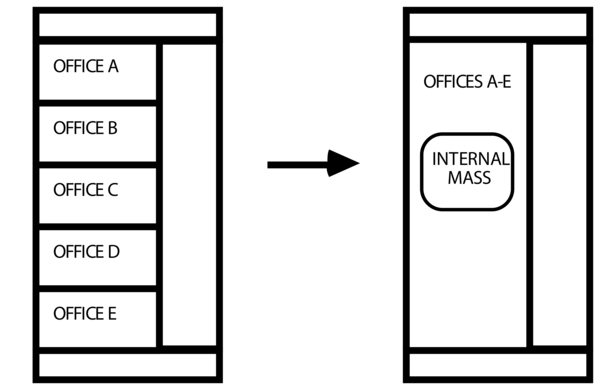
\includegraphics[width=0.9\textwidth, height=0.9\textheight, keepaspectratio=true]{media/image056.png}
\caption{Representing 11 internal walls as internal mass \protect \label{fig:representing-11-internal-walls-as-internal}}
\end{figure}

\textbf{Example}

A five-story building has the same ceiling/floor construction separating each of the levels. Zones that are on floors 2 through 4 may be described using a single piece of internal mass to represent both the floor and ceiling. The construction for this internal mass would be identical to the ceiling/floor construction that would be used to describe separate surfaces and the area of the internal mass surface would be the total surface area of the combined ceilings/floors (i.e.~twice the total floor area).

\paragraph{Field: Name}\label{field-name-21-004}

This is a unique character string associated with the internal mass surface. Though it must be unique from other surface names, it is used primarily for convenience with internal mass surfaces.

\paragraph{Field: Construction Name}\label{field-construction-name-21}

This is the name of the construction (ref: Construction object) used in the surface.

\paragraph{Field: Zone Name}\label{field-zone-name-14}

This is the name of the zone in which the internal mass is represented.

\paragraph{Field: Surface Area}\label{field-surface-area}

This field is the surface area of the internal mass. The area that is specified must be the entire surface area that is exposed to the zone. If both sides of a wall are completely within the same zone, then the area of both sides must be included when describing that internal wall.

IDF examples of Internal Mass surfaces:

\begin{lstlisting}
InternalMass,
  Zn002:IntM001,                !- Surface Name
  INTERIOR,                     !- Construction Name
  DORM ROOMS AND COMMON AREAS,  !- Zone
  408.7734;                     !- Total area exposed to Zone {m2}

InternalMass,
  Zn002:IntM002,                !- Surface Name
  PARTITION02,                  !- Construction Name
  DORM ROOMS AND COMMON AREAS,  !- Zone
  371.6122;                     !- Total area exposed to Zone {m2}
\end{lstlisting}

\subsection{Surface Output Variables/Reports}\label{surface-output-variablesreports}

Note that Surface Outputs from specialized algorithms (such as Effective Moisture Penetration Depth (EMPD), Combined Heat and Moisture Transport (HAMT) and Conduction Finite Difference (CondFD) are discussed under the objects that describe the specialized inputs for these algorithms). You can access them via these links:

\begin{itemize}
\tightlist
\item
  Moisture Penetration Depth (EMPD) Outputs
\item
  Conduction Finite Difference (CondFD) Outputs
\item
  Heat and Moisture (HAMT) Outputs
\end{itemize}

Additionally, the output variables applicable to all heat transfer surfaces:

\begin{lstlisting}
Zone,Sum,Surface Inside Face Heat Balance Calculation Iteration Count []
Zone,Average,Surface Inside Face Temperature [C]
Zone,Average,Surface Outside Face Temperature [C]
Zone,Average,Surface Inside Face Adjacent Air Temperature [C]
Zone,Average,Surface Inside Face Convection Heat Transfer Coefficient [W/m2-K]
Zone,Average,Surface Inside Face Convection Heat Gain Rate [W]
Zone,Average,Surface Inside Face Convection Heat Gain Rate per Area [W/m2]
Zone,Sum,Surface Inside Face Convection Heat Gain Energy [J]
Zone,Average,Surface Inside Face Net Surface Thermal Radiation Heat Gain Rate [W]
Zone,Average,Surface Inside Face Net Surface Thermal Radiation Heat Gain Rate per Area [W/m2]
Zone,Sum,Surface Inside Face Net Surface Thermal Radiation Heat Gain Energy [J]
Zone,Average,Surface Inside Face Solar Radiation Heat Gain Rate [W]
Zone,Average,Surface Inside Face Solar Radiation Heat Gain Rate per Area [W/m2]
Zone,Sum,Surface Inside Face Solar Radiation Heat Gain Energy [J]
Zone,Average,Surface Inside Face Lights Radiation Heat Gain Rate [W]
Zone,Average,Surface Inside Face Lights Radiation Heat Gain Rate per Area [W/m2]
Zone,Sum,Surface Inside Face Lights Radiation Heat Gain Energy [J]
Zone,Average,Surface Inside Face Internal Gains Radiation Heat Gain Rate [W]
Zone,Average,Surface Inside Face Internal Gains Radiation Heat Gain Rate per Area [W/m2]
Zone,Sum,Surface Inside Face Internal Gains Radiation Heat Gain Energy [J]
Zone,Average,Surface Inside Face System Radiation Heat Gain Rate [W]
Zone,Average,Surface Inside Face System Radiation Heat Gain Rate per Area [W/m2]
Zone,Sum,Surface Inside Face System Radiation Heat Gain Energy [J]
Zone,Average,Surface Outside Face Convection Heat Transfer Coefficient [W/m2-K]
Zone,Average,Surface Outside Face Convection Heat Gain Rate [W]
Zone,Average,Surface Outside Face Convection Heat Gain Rate per Area [W/m2]
Zone,Sum,Surface Outside Face Convection Heat Gain Energy [J]
Zone,Average,Surface Outside Face Net Thermal Radiation Heat Gain Rate [W]
Zone,Average,Surface Outside Face Net Thermal Radiation Heat Gain Rate per Area [W/m2]
Zone,Sum,Surface Outside Face Net Thermal Radiation Heat Gain Energy [J]
Zone,Average,Surface Outside Face Thermal Radiation to Air Heat Transfer Coefficient [W/m2-K]
Zone,Average,Surface Outside Face Thermal Radiation to Sky Heat Transfer Coefficient [W/m2-K]
Zone,Average,Surface Outside Face Thermal Radiation to Ground Heat Transfer Coefficient [W/m2-K]
Zone,Average,Surface Inside Face Exterior Windows Incident Beam Solar Radiation Rate [W]
Zone,Sum,Surface Inside Face Exterior Windows Incident Beam Solar Radiation Energy [J]
Zone,Average,Surface Inside Face Exterior Windows Incident Beam Solar Radiation Rate per Area[W/m2]
Zone,Average,Surface Inside Face Interior Windows Incident Beam Solar Radiation Rate [W]
Zone,Average,Surface Inside Face Interior Windows Incident Beam Solar Radiation Rate per Area[W/m2]
Zone, Sum,Surface Inside Face Interior Windows Incident Beam Solar Radiation Energy [J]
Zone,Average,Surface Inside Face Initial Transmitted Diffuse Absorbed Solar Radiation Rate [W]
Zone,Average,Surface Inside Face Initial Transmitted Diffuse Transmitted Out Window Solar Radiation Rate [W]
Zone,Average,Surface Inside Face Absorbed Shortwave Radiation Rate [W]
Zone,Average,Surface Construction Index []
\end{lstlisting}

Output variables applicable to all exterior heat transfer surfaces:

\begin{lstlisting}
Zone,Average,Surface Outside Face Outdoor Air Drybulb Temperature [C]
Zone,Average,Surface Outside Face Outdoor Air Wetbulb Temperature [C]
Zone,Average,Surface Outside Face Outdoor Air Wind Speed [m/s]
Zone,Average,Surface Outside Face Sunlit Area [m2]
Zone,Average,Surface Outside Face Sunlit Fraction \protect\hyperlinksection-1
Zone,Average,Surface Outside Face Incident Solar Radiation Rate per Area[W/m2]
Zone,Average,Surface Outside Face Solar Radiation Heat Gain Rate [W]
Zone,Average,Surface Outside Face Solar Radiation Heat Gain Rate per Area [W/m2]
Zone,Sum,Surface Outside Face Solar Radiation Heat Gain Energy [J]
Zone,Average,Surface Outside Face Incident Beam Solar Radiation Rate per Area[W/m2]
Zone,Average,Surface Outside Face Incident Sky Diffuse Solar Radiation Rate per Area[W/m2]
Zone,Average,Surface Outside Face Incident Ground Diffuse Solar Radiation Rate per Area[W/m2]
Zone,Average,Surface Ext Diff Sol From Bm-To-Diff Refl From Ground[W/m2]
Zone,Average,Surface Outside Face Incident Sky Diffuse Ground Reflected Solar Radiation Rate per Area[W/m2]
Zone,Average,Surface Outside Face Incident Sky Diffuse Surface Reflected Solar Radiation Rate per Area[W/m2]
Zone,Average,Surface Outside Face Incident Beam To Beam Surface Reflected Solar Radiation Rate per Area[W/m2]
Zone,Average,Surface Outside Face Incident Beam To Diffuse Surface Reflected Solar Radiation Rate per Area[W/m2]
Zone,Average,Surface Outside Face Beam Solar Incident Angle Cosine Value[]
Zone,Average,Surface Anisotropic Sky Multiplier []
Zone,Average,Surface Window BSDF Beam Direction Number []
Zone,Average,Surface Window BSDF Beam Theta Angle [rad]
Zone,Average,Surface Window BSDF Beam Phi Angle [rad]
\end{lstlisting}

Output variables applicable to opaque heat transfer surfaces (FLOOR, WALL, ROOF, DOOR). \textbf{Note -- these are advanced variables -- you must read the descriptions and understand before use -- then you must use the Diagnostics object to allow reporting.}

\begin{lstlisting}
Zone,Average,Surface Inside Face Solar Radiation Heat Gain Rate [W]
Zone,Average,Surface Inside Face Solar Radiation Heat Gain Rate per Area [W/m2]
Zone,Sum,Surface Inside Face Solar Radiation Heat Gain Energy [J]
Zone,Average,Surface Inside Face Lights Radiation Heat Gain Rate [W]
Zone,Average,Surface Inside Face Lights Radiation Heat Gain Rate per Area [W/m2]
Zone,Sum,Surface Inside Face Lights Radiation Heat Gain Energy [J]
Zone,Average,Surface Inside Face Conduction Heat Transfer Rate [W]
Zone,Average,Surface Inside Face Conduction Heat Gain Rate [W]
Zone,Average,Surface Inside Face Conduction Heat Loss Rate [W]
Zone,Average,Surface Inside Face Conduction Heat Transfer Rate per Area [W/m2]
Zone,Sum,Surface Inside Face Conduction Heat Transfer Energy [J]
Zone,Average,Surface Outside Face Conduction Heat Transfer Rate [W]
Zone,Average,Surface Outside Face Conduction Heat Gain Rate [W]
Zone,Average,Surface Outside Face Conduction Heat Loss Rate [W]
Zone,Average,Surface Outside Face Conduction Heat Transfer Rate per Area [W/m2]
Zone,Sum,Surface Outside Face Conduction Heat Transfer Energy [J]
Zone,Average,Surface Average Face Conduction Heat Transfer Rate [W]
Zone,Average,Surface Average Face Conduction Heat Gain Rate [W]
Zone,Average,Surface Average Face Conduction Heat Loss Rate [W]
Zone,Average,Surface Average Face Conduction Heat Transfer Rate per Area [W/m2]
Zone,Sum,Surface Average Face Conduction Heat Transfer Energy [J]
Zone,Average,Surface Heat Storage Rate [W]
Zone,Average,Surface Heat Storage Gain Rate [W]
Zone,Average,Surface Heat Storage Loss Rate [W]
Zone,Average,Surface Heat Storage Rate per Area [W/m2]
Zone,Sum,Surface Heat Storage Energy [J]
Zone,Average,Zone Opaque Surface Inside Face Conduction [W]
Zone,Average,Zone Opaque Surface Inside Faces Total Conduction Heat Gain Rate [W]
Zone,Average,Zone Opaque Surface Inside Faces Total Conduction Heat Loss Rate [W]
Zone,Sum,Zone Opaque Surface Inside Faces Total Conduction Heat Gain Energy [J]
Zone,Sum,Zone Opaque Surface Inside Faces Total Conduction Heat Loss Energy [J]
Zone,Average,Zone Opaque Surface Outside Face Conduction [W]
Zone,Average,Zone Opaque Surface Outside Face Conduction Gain[W]
Zone,Average,Zone Opaque Surface Outside Face Conduction Loss[W]
Zone,Average, Surface Inside Face Beam Solar Radiation Heat Gain Rate [W]
\end{lstlisting}

\subsection{Window Output Variables}\label{window-output-variables}

Output variables applicable only to exterior windows and glass doors:

\begin{lstlisting}
Zone,Average,Zone Windows Total Transmitted Solar Radiation Rate [W]
Zone,Sum,Zone Transmitted Solar Energy [J]
Zone,Average,Zone Windows Total Heat Gain Rate [W]
Zone,Sum,Zone Windows Total Heat Gain Energy [J]
Zone,Average,Zone Windows Total Heat Loss Rate [W]
Zone,Sum,Zone Windows Total Heat Loss Energy [J]
Zone,Average,Zone Exterior Windows Total Transmitted Beam Solar Radiation Rate [W]
Zone,Sum,Zone Exterior Windows Total Transmitted Beam Solar Radiation Energy [J]
Zone,Average,Zone Interior Windows Total Transmitted Beam Solar Radiation Rate [W]
Zone,Sum,Zone Interior Windows Total Transmitted Beam Solar Radiation Energy [J]
Zone,Average,Zone Exterior Windows Total Transmitted Diffuse Solar Radiation Rate [W]
Zone,Sum,Zone Exterior Windows Total Transmitted Diffuse Solar Radiation Energy [J]
Zone,Average,Zone Interior Windows Total Transmitted Diffuse Solar Radiation Rate [W]
Zone,Average,Surface Window Total Glazing Layers Absorbed Solar Radiation Rate [W]
Zone,Average,Surface Window Total Glazing Layers Absorbed Shortwave Radiation Rate [W]
Zone,Sum,Surface Window Total Glazing Layers Absorbed Solar Radiation Energy [J]
Zone,Average,Surface Window Shading Device Absorbed Solar Radiation Rate [W]
Zone,Sum,Surface Window Shading Device Absorbed Solar Radiation Energy [J]
Zone,Average, Surface Window Transmitted Solar Radiation Rate [W]
Zone,Sum,Surface Window Transmitted Solar Radiation Energy [J]
Zone,Average,Surface Window Transmitted Beam Solar Radiation Rate [W]
Zone,Average,Surface Window Transmitted Beam To Beam Solar Radiation Rate [W]
Zone,Average,Surface Window Transmitted Beam To Diffuse Solar Radiation Rate [W]
Zone,Sum,Surface Window Transmitted Beam Solar Radiation Energy [J]
Zone,Sum,Surface Window Transmitted Beam To Beam Solar Radiation Energy [J]
Zone,Sum,Surface Window Transmitted Beam To Diffuse Solar Radiation Energy [J]
Zone,Average,Surface Window Transmitted Diffuse Solar Radiation Rate [W]
Zone,Sum,Surface Window Transmitted Diffuse Solar Radiation Energy [J]
Zone,Average,Surface Window System Solar Transmittance []
Zone,Average,Surface Window System Solar Absorptance []
Zone,Average,Surface Window System Solar Reflectance []
Zone,Average,Surface Window Gap Convective Heat Transfer Rate [W]
Zone,Sum,Surface Window Gap Convective Heat Transfer Energy [J]
Zone,Average,Surface Window Heat Gain Rate [W]
Zone,Sum,Surface Window Heat Gain Energy [J]
Zone,Average,Surface Window Heat Loss Rate [W]
Zone,Sum,Surface Window Heat Loss Energy [J]
Zone,Average,Surface Window Net Heat Transfer Rate [W]
Zone,Sum,Surface Window Net Heat Transfer Energy [J]
Zone,Average,Surface Window Glazing Beam to Beam Solar Transmittance[]
Zone,Average,Surface Window Glazing Beam to Diffuse Solar Transmittance []
Zone,Average,Surface Window Glazing Diffuse to Diffuse Solar Transmittance[]
Zone,Average,Surface Window Model Solver Iteration Count []
Zone,Average,Surface Window Solar Horizontal Profile Angle[deg]
Zone,Average,Surface Window Solar Vertical Profile Angle[deg]
Zone,Average,Surface Window Outside Reveal Reflected Beam Solar Radiation Rate [W]
Zone,Sum,Surface Window Outside Reveal Reflected Beam Solar Radiation Energy
Zone,Average,Surface Window Inside Reveal Reflected Beam Solar Radiation Rate [W]
Zone,Sum,Surface Window Inside Reveal Reflected Beam Solar Radiation Energy [J]
Zone,Average,Surface Window Inside Reveal Absorbed Beam Solar Radiation Rate [W]
Zone,Average,Surface Window Inside Face Glazing Condensation Status []
Zone,Average,Surface Window Inside Face Frame Condensation Status []
Zone,Average,Surface Window Inside Face Divider Condensation Status []
Zone,Average,Surface Shading Device Is On Time Fraction[]
Zone,Average,Surface Window Blind Slat Angle [deg]
Zone,Average,Surface Window Blind Beam to Beam Solar Transmittance[]
Zone,Average,Surface Window Blind Beam to Diffuse Solar Transmittance[]
Zone,Average,Surface Window Blind Diffuse to Diffuse Solar Transmittance[]
Zone,Average,Surface Window Blind and Glazing System Beam Solar Transmittance[]
Zone,Average,Surface Window Blind and Glazing System Diffuse Solar Transmittance[]
Zone,Average,Surface Window Screen Beam to Beam Solar Transmittance []
Zone,Average,Surface Window Screen Beam to Diffuse Solar Transmittance []
Zone,Average,Surface Window Screen Diffuse to Diffuse Solar Transmittance []
Zone,Average,Surface Window Screen and Glazing System Beam Solar Transmittance []
Zone,Average,Surface Window Screen and Glazing System Diffuse Solar Transmittance []
Zone,State,Surface Storm Window On Off Status []
Zone,Average,Surface Window Inside Face Frame and Divider Zone Heat Gain Rate [W]
Zone,Average,Surface Window Frame Heat Gain Rate [W]
Zone,Average,Surface Window Frame Heat Loss Rate [W]
Zone,Average,Surface Window Divider Heat Gain Rate [W]
Zone,Average,Surface Window Divider Heat Loss Rate [W]
Zone,Average,Surface Window Frame Inside Temperature [C]
Zone,Average,Surface Window Frame Outside Temperature [C]
Zone,Average,Surface Window Divider Inside Temperature [C]
Zone,Average,Surface Window Divider Outside Temperature [C]
\end{lstlisting}

If the user requests to display advanced report/output variables (e.g.~see Output:Diagnostics keyword DisplayAdvancedReportVariables) the the following additional output variables are available for exterior windows and glass doors

\begin{lstlisting}
Zone,Average,Surface Window Inside Face Glazing Zone Convection Heat Gain Rate [W]
Zone,Average,Surface Window Inside Face Glazing Net Infrared Heat Transfer Rate [W]
Zone,Average,Surface Window Shortwave from Zone Back Out Window Heat Transfer Rate [W]
Zone,Average,Surface Window Inside Face Frame and Divider Zone Heat Gain Rate [W]
Zone,Average,Surface Window Inside Face Gap between Shade and Glazing Zone Convection Heat Gain Rate [W]
Zone,Average,Surface Window Inside Face Shade Zone Convection Heat Gain Rate [W]
Zone,Average,Surface Window Inside Face Shade Net Infrared Heat Transfer Rate [W]
\end{lstlisting}

Output variables applicable only to interior windows and glass doors:

\begin{lstlisting}
Zone,Average, Surface Window Transmitted Beam Solar Radiation Rate [W]
Zone,Sum,Surface Window Transmitted Beam Solar Radiation Energy [J]
\end{lstlisting}

If the user requests to display advanced report/output variables (e.g.~see Output:Diagnostics keyword DisplayAdvancedReportVariables) the the following additional output variable is available for Equivalent Layer Window;

\begin{lstlisting}
Zone,Average, Surface Window Inside Face Other Convection Heat Gain Rate [W]
\end{lstlisting}

Output variables applicable to interior and exterior windows and doors are:

\begin{lstlisting}
Zone,Average,Surface Window Total Absorbed Shortwave Radiation Rate Layer <x> [W]
Zone,Average,Surface Window Front Face Temperature Layer <x> [C]
Zone,Average,Surface Window Back Face Temperature Layer <x> [C]
\end{lstlisting}

\subsubsection{Surface Window Total Absorbed Shortwave Radiation Rate Layer \textless{}x\textgreater{} {[}W{]}}\label{surface-window-total-absorbed-shortwave-radiation-rate-layer-x-w}

This will output shortwave radiation absorbed in a window layer. The key values for this output variable are the surface name. Layers are numbered from the outside to the inside of the surface. The full listing will appear in the RDD file.

\subsubsection{Surface Window Front Face Temperature Layer \textless{}x\textgreater{} {[}C{]}}\label{surface-window-front-face-temperature-layer-x-c}

This will output a temperature for the front face of the layer. The layer front face is considered to be the face closest to the outside environment. The full listing will appear in the RDD file.

\subsubsection{Surface Window Back Face Temperature Layer \textless{}x\textgreater{} {[}C{]}}\label{surface-window-back-face-temperature-layer-x-c}

This will output a temperature for the back face of the layer. The layer back face is considered to be the face closest to the inside environment. The full listing will appear in the RDD file.

\subsection{Surface Output Variables (all heat transfer surfaces)}\label{surface-output-variables-all-heat-transfer-surfaces}

The various output variables related to surface heat transfer are organized around the inside and outside face of each surface. The zone heat balance model draws energy balances at each side, or face, of a surface and so each surface essentially has two sets of results. The inside face is the side of a heat transfer surface that faces toward the thermal zone. The outside face is the side of a heat transfer surface that faces away from the thermal zone, typically facing outdoors. The Key Value for these is generally the user-defined name of the surface.

\subsubsection{Surface Inside Face Heat Balance Calculation Iteration Count {[]}}\label{surface-inside-face-heat-balance-calculation-iteration-count}

This output is the number of iterations used in a part of the solution for surface heat transfer that accounts for thermal radiation heat transfer between zone surfaces. This is simply a counter on the iteration loop for inside face surface modeling. There is only one instance of this output in a given run and the Key Value is ``Simulation.''

\subsubsection{Surface Inside Face Temperature {[}C{]}}\label{surface-inside-face-temperature-c}

This is the temperature of the surface's inside face, in degrees Celsius. Former Name: Prior to version 7.1 this output was called Surface Inside Temperature.

\subsubsection{Surface Outside Face Temperature {[}C{]}}\label{surface-outside-face-temperature-c}

This is the temperature of the surface's outside face, in degrees Celsius. Former Name: Prior to version 7.1, this output was called Surface Outside Temperature.

\subsubsection{Surface Inside Face Adjacent Air Temperature {[}C{]}}\label{surface-inside-face-adjacent-air-temperature-c}

This is the effective bulk air temperature used for modeling the inside surface convection heat transfer. This is the same as the zone mean air temperature when using the mixing model for roomair. However, if more advanced roomair models are used, this variable will report the air temperature predicted by the roomair model as it was used in the surface heat balance model calculations. Former Name: Prior to version 7.1, this output was called Surface Int Adjacent Air Temperature.

\subsubsection{Surface Inside Face Convection Heat Gain Rate {[}W{]}}\label{surface-inside-face-convection-heat-gain-rate-w}

\subsubsection{Surface Inside Face Convection Heat Gain Rate per Area {[}W/m2{]}}\label{surface-inside-face-convection-heat-gain-rate-per-area-wm2}

\subsubsection{Surface Inside Face Convection Heat Gain Energy {[}J{]}}\label{surface-inside-face-convection-heat-gain-energy-j}

These ``inside face convection heat gain'' output variables describe the heat transferred by convection between the inside face and the zone air. The values can be positive or negative with positive indicating heat is being added to the surface's face by convection. Different versions of the report are available including the basic heat gain rate (W), and a per unit area flux (W/m2), and an energy version (J).

Former Name: Prior to version 7.1, these outputs were called ``Surface Int Convection Heat *'' and had used the opposite sign convention.

\subsubsection{Surface Inside Face Convection Heat Transfer Coefficient {[}W/m2-K{]}}\label{surface-inside-face-convection-heat-transfer-coefficient-wm2-k}

This is the coefficient that describes the convection heat transfer. It is the value of ``Hc'' in the classic convection model Q = Hc* A* (T -- T). This is the result of the surface convection algorithm used for the inside face. Former Name: Prior to version 7.1, this output was called ``Surface Int Convection Coeff.''

\subsubsection{Surface Inside Face Net Surface Thermal Radiation Heat Gain Rate {[}W{]}}\label{surface-inside-face-net-surface-thermal-radiation-heat-gain-rate-w}

\subsubsection{Surface Inside Face Net Surface Thermal Radiation Heat Gain Rate per Area {[}W/m2{]}}\label{surface-inside-face-net-surface-thermal-radiation-heat-gain-rate-per-area-wm2}

\subsubsection{Surface Inside Face Net Surface Thermal Radiation Heat Gain Energy {[}J{]}}\label{surface-inside-face-net-surface-thermal-radiation-heat-gain-energy-j}

These ``inside face net surface thermal radiation heat gain'' output variables describe the heat transferred by longwave infrared thermal radiation exchanges between the inside faces of other surfaces in the zone. The values can be positive or negative with positive indicating heat is being added to the surface's face by thermal radiation. Different versions of the report are available including the basic heat gain rate (W), and a per unit area flux (W/m2), and an energy version (J).

\subsubsection{Surface Inside Face Solar Radiation Heat Gain Rate {[}W{]}}\label{surface-inside-face-solar-radiation-heat-gain-rate-w}

\subsubsection{Surface Inside Face Solar Radiation Heat Gain Rate per Area {[}W/m2{]}}\label{surface-inside-face-solar-radiation-heat-gain-rate-per-area-wm2}

\subsubsection{Surface Inside Face Solar Radiation Heat Gain Energy {[}J{]}}\label{surface-inside-face-solar-radiation-heat-gain-energy-j}

These ``inside face solar radiation heat gain'' output variables describe the heat transferred by solar radiation onto the inside face. The values are always positive and indicate heat is being added to the surface's face by solar radiation. This is sunlight that has entered the zone through a window and been absorbed on the inside face of the surface. Different versions of the report are available including the basic heat gain rate (W), and a per unit area flux (W/m2), and an energy version (J).

\subsubsection{Surface Inside Face Lights Radiation Heat Gain Rate {[}W{]}}\label{surface-inside-face-lights-radiation-heat-gain-rate-w}

\subsubsection{Surface Inside Face Lights Radiation Heat Gain Rate per Area {[}W/m2{]}}\label{surface-inside-face-lights-radiation-heat-gain-rate-per-area-wm2}

\subsubsection{Surface Inside Face Lights Radiation Heat Gain Energy {[}J{]}}\label{surface-inside-face-lights-radiation-heat-gain-energy-j}

These ``inside face lights radiation heat gain'' output variables describe the heat transferred by shortwave radiation onto the inside face. The values are always positive and indicate heat is being added to the surface's face by shortwave radiation that emanated from electric lighting equipment and was absorbed by the surface. Different versions of the report are available including the basic heat gain rate (W), and a per unit area flux (W/m2), and an energy version (J).

\subsubsection{Surface Inside Face Internal Gains Radiation Heat Gain Rate {[}W{]}}\label{surface-inside-face-internal-gains-radiation-heat-gain-rate-w}

\subsubsection{Surface Inside Face Internal Gains Radiation Heat Gain Rate per Area {[}W/m2{]}}\label{surface-inside-face-internal-gains-radiation-heat-gain-rate-per-area-wm2}

\subsubsection{Surface Inside Face Internal Gains Radiation Heat Gain Energy {[}J{]}}\label{surface-inside-face-internal-gains-radiation-heat-gain-energy-j}

These ``inside face internal gains radiation heat gain'' output variables describe the heat transferred by longwave infrared thermal radiation onto the inside face that emanated from internal gains such as lights, electric equipment, and people. The values are always positive and indicate heat is being added to the surface's face by the absorption of longwave thermal radiation. Different versions of the report are available including the basic heat gain rate (W), and a per unit area flux (W/m2), and an energy version (J).

\subsubsection{Surface Inside Face System Radiation Heat Gain Rate {[}W{]}}\label{surface-inside-face-system-radiation-heat-gain-rate-w}

\subsubsection{Surface Inside Face System Radiation Heat Gain Rate per Area {[}W/m2{]}}\label{surface-inside-face-system-radiation-heat-gain-rate-per-area-wm2}

\subsubsection{Surface Inside Face System Radiation Heat Gain Energy {[}J{]}}\label{surface-inside-face-system-radiation-heat-gain-energy-j}

These ``inside face system radiation heat gain'' output variables describe the heat transferred by infrared thermal radiation onto the inside face that emanated from HVAC equipment such as baseboard heaters or high-temperature radiant heating panels. The values are always positive and indicate heat is being added to the surface's face by the absorption of thermal radiation. Different versions of the report are available including the basic heat gain rate (W), and a per unit area flux (W/m2), and an energy version (J).

\subsubsection{Surface Outside Face Convection Heat Gain Rate {[}W{]}}\label{surface-outside-face-convection-heat-gain-rate-w}

\subsubsection{Surface Outside Face Convection Heat Gain Rate per Area {[}W/m2{]}}\label{surface-outside-face-convection-heat-gain-rate-per-area-wm2}

\subsubsection{Surface Outside Face Convection Heat Gain Energy {[}J{]}}\label{surface-outside-face-convection-heat-gain-energy-j}

These ``outside face convection'' output variables describe heat transferred by convection between the outside face and the surrounding air. The values can be positive or negative with positive values indicating heat is added to the surface face by convection heat transfer. Different versions of the report are available including the basic heat gain rate (W), and a per unit area flux (W/m\(^{2}\)), and an energy version (J).

Former Name: Prior to version 7.1, these outputs were called ``Surface Ext Convection Heat *'' and used the opposite sign convention.

\subsubsection{Surface Outside Face Convection Heat Transfer Coefficient {[}W/m2-K{]}}\label{surface-outside-face-convection-heat-transfer-coefficient-wm2-k}

This is the coefficient that describes the convection heat transfer. It is the value of ``Hc'' in the classic convection model Q = Hc* A* (T -- T). This is the result of the surface convection algorithm used for the outside face. Former Name: Prior to Version 7.1, this output was called ``Surface Ext Convection Coeff.''

\subsubsection{Surface Outside Face Net Thermal Radiation Heat Gain Rate {[}W{]}}\label{surface-outside-face-net-thermal-radiation-heat-gain-rate-w}

\subsubsection{Surface Outside Face Net Thermal Radiation Heat Gain Rate per Area {[}W/m2{]}}\label{surface-outside-face-net-thermal-radiation-heat-gain-rate-per-area-wm2}

\subsubsection{Surface Outside Face Net Thermal Radiation Heat Gain Energy {[}J{]}}\label{surface-outside-face-net-thermal-radiation-heat-gain-energy-j}

These ``outside face net thermal radiation'' output variables describe the heat transferred by longwave infrared thermal radiation exchanges between the surface and the surroundings of the outside face. This is the net of all forms of longwave thermal infrared radiation heat transfer. The values can be positive or negative with positive indicating the net addition of heat to the outside face. Different versions of the report are available including the basic heat gain rate (W), and a per unit area flux (W/m2), and an energy version (J).

Former Name: Prior to version 7.1, these outputs were called ``Surface Ext Thermal Radiation Heat *'' and used the opposite sign convention.

\subsubsection{Surface Inside Face Exterior Windows Incident Beam Solar Radiation Rate {[}W{]}}\label{surface-inside-face-exterior-windows-incident-beam-solar-radiation-rate-w}

\subsubsection{Surface Inside Face Exterior Windows Incident Beam Solar Radiation Rate per Area {[}W/m2{]}}\label{surface-inside-face-exterior-windows-incident-beam-solar-radiation-rate-per-area-wm2}

\subsubsection{Surface Inside Face Exterior Windows Incident Beam Solar Radiation Energy {[}J{]}}\label{surface-inside-face-exterior-windows-incident-beam-solar-radiation-energy-j}

Beam solar radiation from the exterior windows in a zone incident on the inside face of a surface in the zone. If Solar Distribution in the BUILDING object is equal to MinimalShadowing or FullExterior, it is assumed that all beam solar from exterior windows falls on the floor. In this case the value of this output variable can be greater than zero only for floor surfaces. If Solar Distribution equals FullInteriorExterior the program tracks where beam solar from exterior windows falls inside the zone, in which case the value of this variable can be greater than zero for floor as well as wall surfaces. Different versions of the report are available including the basic incident rate (W), a per unit area flux (W/m2), and an energy version (J).

\subsubsection{Surface Inside Face Interior Windows Incident Beam Solar Radiation Rate {[}W{]}}\label{surface-inside-face-interior-windows-incident-beam-solar-radiation-rate-w}

\subsubsection{Surface Inside Face Interior Windows Incident Beam Solar Radiation Rate per Area {[}W/m2{]}}\label{surface-inside-face-interior-windows-incident-beam-solar-radiation-rate-per-area-wm2}

\subsubsection{Surface Inside Face Interior Windows Incident Beam Solar Radiation Energy {[}J{]}}\label{surface-inside-face-interior-windows-incident-beam-solar-radiation-energy-j}

Beam solar radiation from the interior (i.e., interzone) windows in a zone incident on the inside face of a surface in the zone. This value is calculated only if Solar Distribution in the BUILDING object is equal to FullInteriorExterior. However, the program does not track where this radiation falls. Instead, it is treated by the program as though it were diffuse radiation uniformly distributed over all of the zone surfaces. See \textbf{Figure~\ref{fig:beam-solar-radiation-entering-a-zone-through}}. Different versions of the report are available including the basic incident rate (W), a per unit area flux (W/m2), and an energy version (J).

\begin{figure}[hbtp] % fig 31
\centering
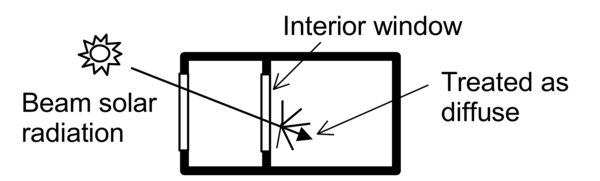
\includegraphics[width=0.9\textwidth, height=0.9\textheight, keepaspectratio=true]{media/image057.png}
\caption{Beam solar radiation entering a zone through an interior window is distributed inside the zone as though it were diffuse radiation. \protect \label{fig:beam-solar-radiation-entering-a-zone-through}}
\end{figure}

\subsubsection{Surface Inside Face Initial Transmitted Diffuse Absorbed Solar Radiation Rate {[}W{]}}\label{surface-inside-face-initial-transmitted-diffuse-absorbed-solar-radiation-rate-w}

As of Version 2.1, diffuse solar transmitted through exterior and interior windows is no longer uniformly distributed. Instead, it is distributed according to the approximate view factors between the transmitting window and all other heat transfer surfaces in the zone. This variable is the amount of transmitted diffuse solar that is initially absorbed on the inside of each heat transfer surface. The portion of this diffuse solar that is reflected by all surfaces in the zone is subsequently redistributed uniformly to all heat transfer surfaces in the zone, along with interior reflected beam solar and shortwave radiation from lights. The total absorbed shortwave radiation is given by the next variable.

\subsubsection{Surface Inside Face Absorbed Shortwave Radiation Rate {[}W{]}}\label{surface-inside-face-absorbed-shortwave-radiation-rate-w}

As of Version 2.1, the previous variable plus absorbed shortwave radiation from uniformly distributed initially-reflected diffuse solar, reflected beam solar, and shortwave radiation from lights. This sum is the power of all sources of solar and visible radiation absorbed by the surface at the inside face.

\subsubsection{Surface Construction Index {[]}}\label{surface-construction-index}

The variable reports an index that points to specific Construction. The variable is an additional output variable when Output:Diagnostics, DisplayAdvancedReportVariables; is given in an input file.

In order to find a corresponding construction using the index, following steps are suggested:

1. Find a surface name from Surface Construction Index in the .csv file

2. Search the surface name in lines starting with HeatTransfer Surface in the .eio file

3. The seventh item is the construction name with matched surface name. 
 
\subsection{Surface Output Variables (exterior heat transfer surfaces)}\label{surface-output-variables-exterior-heat-transfer-surfaces}

\subsubsection{Surface Outside Face Outdoor Air Drybulb Temperature {[}C{]}}\label{surface-outside-face-outdoor-air-drybulb-temperature-c}

The outdoor air dry-bulb temperature calculated at the height above ground of the surface centroid. Former Name: Prior to version 7.1, this output was called ``Surface Ext Outdoor Dry Bulb.''

\subsubsection{Surface Outside Face Outdoor Air Wetbulb Temperature {[}C{]}}\label{surface-outside-face-outdoor-air-wetbulb-temperature-c}

The outdoor air wet-bulb temperature calculated at the height above ground of the surface centroid. Former Name: Prior to version 7.1, this output was called ``Surface Ext Outdoor Wet Bulb.''

\subsubsection{Surface Outside Face Outdoor Air Wind Speed {[}m/s{]}}\label{surface-outside-face-outdoor-air-wind-speed-ms}

The outdoor wind speed calculated at the height above ground of the surface centroid. Former Name: Prior to version 7.1, this output was called ``Surface Ext Wind Speed.''

\subsubsection{Surface Outside Face Sunlit Area {[}m2{]}}\label{surface-outside-face-sunlit-area-m2}

The outside area of an exterior surface that is illuminated by (unreflected) beam solar radiation.

\subsubsection{Surface Outside Face Sunlit Fraction {[]}}\label{surface-outside-face-sunlit-fraction}

The fraction of the outside area of an exterior surface that is illuminated by (unreflected) beam solar radiation. Equals Surface Outside Face Sunlit Area divided by total surface area.

\subsubsection{Surface Outside Face Thermal Radiation to Air Heat Transfer Coefficient {[}W/m2-K{]}}\label{surface-outside-face-thermal-radiation-to-air-heat-transfer-coefficient-wm2-k}

This is the coefficient that describes thermal radiation heat transfer between the outside face and the air mass surrounding the surface. It is the value of ``Hr'' in the classic linearized model for thermal radiation Q = Hr * A * (T\_surf -- T\_surfodb) when applied to the ambient air. Where T\_surf = Surface Outside Face Temperature, and T\_surfodb = Surface Outside Face Outdoor Air Drybulb Temperature. Former Name: Prior to version 7.1, this output was called ``Surface Ext Rad to Air Coeff.''

\subsubsection{Surface Outside Face Thermal Radiation to Sky Heat Transfer Coefficient {[}W/m2-K{]}}\label{surface-outside-face-thermal-radiation-to-sky-heat-transfer-coefficient-wm2-k}

This is the coefficient that describes thermal radiation heat transfer between the outside face and the sky surrounding the surface. It is the value of ``Hr'' in the classic linearized model for thermal radiation Q = Hr * A * (T\_surf -- T\_sky) when applied to the sky. Where T\_surf = Surface Outside Face Temperature, and T\_sky = Site Sky Temperature. Former Name: Prior to version 7.1, this output was called ``Surface Ext Rad to Sky Coeff.''

\subsubsection{Surface Outside Face Thermal Radiation to Ground Heat Transfer Coefficient {[}W/m2-K{]}}\label{surface-outside-face-thermal-radiation-to-ground-heat-transfer-coefficient-wm2-k}

This is the coefficient that describes thermal radiation heat transfer between the outside face and the ground surrounding the surface. It is the value of ``Hr'' in the classic linearized model for thermal radiation Q = Hr * A * (T\_surf -- T\_odb) when applied to the ground. Where T\_surf = Surface Outside Face Temperature, and T\_odb = Site Outdoor Air Drybulb Temperature (used as an approximation for the ground surface temperature). Former Name: Prior to version 7.1, this output was called ``Surface Ext Rad to Ground Coeff.''

\subsubsection{Surface Outside Face Solar Radiation Heat Gain Rate {[}W{]}}\label{surface-outside-face-solar-radiation-heat-gain-rate-w}

\subsubsection{Surface Outside Face Solar Radiation Heat Gain Rate per Area {[}W/m2{]}}\label{surface-outside-face-solar-radiation-heat-gain-rate-per-area-wm2}

\subsubsection{Surface Outside Face Solar Radiation Heat Gain Energy {[}J{]}}\label{surface-outside-face-solar-radiation-heat-gain-energy-j}

These ``outside face solar radiation'' output variables describe the heat transferred by the absorption of solar radiation at the outside face. This is the result of incident solar radiation being absorbed at the surface face. The values are always positive.

\subsubsection{Surface Outside Face Incident Solar Radiation Rate per Area {[}W/m2{]}}\label{surface-outside-face-incident-solar-radiation-rate-per-area-wm2}

The total solar radiation incident on the outside of an exterior surface. It is the sum of:

\begin{itemize}
\item
  Surface Outside Face Incident Beam Solar Radiation Rate per Area
\item
  Surface Outside Face Incident Sky Diffuse Solar Radiation Rate per Area
\item
  Surface Outside Face Incident Ground Diffuse Solar Radiation Rate per Area
\item
  Surface Outside Face Incident Sky Diffuse Surface Reflected Solar Radiation Rate per Area
\item
  Surface Outside Face Incident Beam To Beam Surface Reflected Solar Radiation Rate per Area
\item
  Surface Outside Face Incident Sky Diffuse Surface Reflected Solar Radiation Rate per Area
\end{itemize}

\subsubsection{Surface Outside Face Incident Beam Solar Radiation Rate per Area {[}W/m2{]}}\label{surface-outside-face-incident-beam-solar-radiation-rate-per-area-wm2}

The solar beam radiation incident on the outside of an exterior surface, including the effects of shadowing, if present. The beam here is that directly from the sun; it excludes beam specularly reflected from obstructions.

\subsubsection{Surface Outside Face Incident Sky Diffuse Solar Radiation Rate per Area {[}W/m2{]}}\label{surface-outside-face-incident-sky-diffuse-solar-radiation-rate-per-area-wm2}

The solar diffuse radiation from the sky incident on the outside of an exterior surface, including the effects of shadowing, if present.

\subsubsection{Surface Outside Face Incident Ground Diffuse Solar Radiation Rate per Area {[}W/m2{]}}\label{surface-outside-face-incident-ground-diffuse-solar-radiation-rate-per-area-wm2}

The solar diffuse radiation incident on the outside of an exterior surface that arises from reflection of beam solar and sky diffuse solar from the ground. This is the sum of the next two output variables, ``Surface Outside Face Incident Beam To Diffuse Ground Reflected Solar Radiation Rate per Area'' and ``Surface Outside Face Incident Sky Diffuse Ground Reflected Solar Radiation Rate per Area.'' The reflected solar radiation from the ground is assumed to be diffuse and isotropic (there is no specular component).

If ``Reflections'' option is not chosen in the Solar Distribution Field in the BUILDING object, the effects of shadowing are accounted for by the user-specified value of View Factor to Ground for the surface. If ``Reflections'' option is chosen, the program determines the effects of shadowing, including time-varying shadowing of the ground plane by the building itself.

\subsubsection{Surface Outside Face Incident Beam To Diffuse Ground Reflected Solar Radiation Rate per Area {[}W/m2{]}}\label{surface-outside-face-incident-beam-to-diffuse-ground-reflected-solar-radiation-rate-per-area-wm2}

The solar diffuse radiation incident on the outside of an exterior surface that arises from beam-to-diffuse reflection from the ground. It is assumed that there is no beam-to-beam (specular) component. The beam here is that directly from the sun; it excludes beam specularly reflected from obstructions.

\subsubsection{Surface Outside Face Incident Sky Diffuse Ground Reflected Solar Radiation Rate per Area {[}W/m2{]}}\label{surface-outside-face-incident-sky-diffuse-ground-reflected-solar-radiation-rate-per-area-wm2}

The solar diffuse radiation incident on the outside of an exterior surface that arises from sky diffuse solar reflection from the ground. The sky diffuse here is that directly from the sky; it excludes reflection of sky diffuse from obstructions.

\subsubsection{Surface Outside Face Incident Sky Diffuse Surface Reflected Solar Radiation Rate per Area {[}W/m2{]}}\label{surface-outside-face-incident-sky-diffuse-surface-reflected-solar-radiation-rate-per-area-wm2}

The solar diffuse radiation incident on the outside of an exterior surface that arises from sky diffuse reflection from one or more obstructions. This value will be non-zero only if ``Reflections'' option is chosen in the BUILDING object.

\subsubsection{Surface Outside Face Incident Beam To Beam Surface Reflected Solar Radiation Rate per Area {[}W/m2{]}}\label{surface-outside-face-incident-beam-to-beam-surface-reflected-solar-radiation-rate-per-area-wm2}

The solar beam radiation incident on the outside of an exterior surface that arises from beam-to-beam (specular) reflection from one or more obstructions. This value will be non-zero only if ``Reflections'' option is chosen in the BUILDING object. For windows, the program treats this beam radiation as diffuse radiation in calculating its transmission and absorption.

\subsubsection{Surface Outside Face Incident Beam To Diffuse Surface Reflected Solar Radiation Rate per Area {[}W/m2{]}}\label{surface-outside-face-incident-beam-to-diffuse-surface-reflected-solar-radiation-rate-per-area-wm2}

The solar diffuse radiation incident on the outside of an exterior surface that arises from beam-to-diffuse reflection from building shades or building surfaces. This value will be non-zero only if ``Reflections'' option is chosen in the BUILDING object.

\subsubsection{Surface Outside Face Beam Solar Incident Angle Cosine Value {[]}}\label{surface-outside-face-beam-solar-incident-angle-cosine-value}

The cosine of the angle of incidence of (unreflected) beam solar radiation on the outside of an exterior surface. The value varies from 0.0 for beam parallel to the surface (incidence angle = 90\(^{O}\)) to 1.0 for beam perpendicular to the surface (incidence angle = 0\(^{O}\)). Negative values indicate the sun is behind the surface, i.e the surface does not see the sun.

\subsubsection{Surface Anisotropic Sky Multiplier {[]}}\label{surface-anisotropic-sky-multiplier}

This is the view factor multiplier for diffuse sky irradiance on exterior surfaces taking into account the anisotropic radiance of the sky. The diffuse sky irradiance on a surface is given by Anisotropic Sky Multiplier * Diffuse Solar Irradiance.

\subsubsection{Surface Window BSDF Beam Direction Number {[]}}\label{surface-window-bsdf-beam-direction-number}

\subsubsection{Surface Window BSDF Beam Phi Angle {[}rad{]}}\label{surface-window-bsdf-beam-phi-angle-rad}

\subsubsection{Surface Window BSDF Beam Theta Angle {[}rad{]}}\label{surface-window-bsdf-beam-theta-angle-rad}

\subsection{Opaque Surface Output Variables}\label{opaque-surface-output-variables}

The following variables apply only to opaque surfaces, where an opaque surface is considered here to be an exterior or interzone heat transfer surface of class FLOOR, WALL, ROOF or DOOR. \textbf{Note -- these are advanced variables -- you must read the descriptions and understand before use -- then you must use the} \textbf{Output:Diagnostics} \textbf{object to allow reporting.}

\subsubsection{Surface Inside Face Conduction Heat Transfer Rate {[}W{]}}\label{surface-inside-face-conduction-heat-transfer-rate-w}

\subsubsection{Surface Inside Face Conduction Heat Transfer Rate per Area {[}W/m2{]}}\label{surface-inside-face-conduction-heat-transfer-rate-per-area-wm2}

\subsubsection{Surface Inside Face Conduction Heat Gain Rate {[}W{]}}\label{surface-inside-face-conduction-heat-gain-rate-w}

\subsubsection{Surface Inside Face Conduction Heat Loss Rate {[}W{]}}\label{surface-inside-face-conduction-heat-loss-rate-w}

These ``inside face conduction'' output variables describe heat flow by conduction right at the inside face of an opaque heat transfer surface. A positive value means that the conduction is from just inside the inside face toward the inside face. A negative value means that the conduction is from the inside face into the core of the heat transfer surface.

Note that Inside Face Conduction, when positive, does \textbf{not} indicate the heat flow from the surface to the zone air, which is governed by the inside face convection coefficient and the difference in temperature between the inside face and the zone air.

Different versions of the reports are available. The basic heat gain rate (W) and a per unit area flux (W/m\(^{2}\)) can have positive or negative values with the sign convention that positive indicates heat flowing toward the face itself. There are also directed ``gain'' and ``loss'' versions that have only positive values or zero when the heat flow direction opposes.

Former Name: Prior to version 7.1, these outputs were called ``Opaque Surface Inside Face Conduction *.''

Former Name: For Conduction Finite Difference simulations (CondFD), CondFD Inside Surface Heat Flux is replaced with Surface Inside Face Conduction Heat Transfer Rate Per Area. Likewise for CondFD Inside Heat Flux to Surface.

\subsubsection{Surface Outside Face Conduction Heat Transfer Rate {[}W{]}}\label{surface-outside-face-conduction-heat-transfer-rate-w}

\subsubsection{Surface Outside Face Conduction Heat Transfer Rate per Area {[}W/m2{]}}\label{surface-outside-face-conduction-heat-transfer-rate-per-area-wm2}

\subsubsection{Surface Outside Face Conduction Heat Gain Rate {[}W{]}}\label{surface-outside-face-conduction-heat-gain-rate-w}

\subsubsection{Surface Outside Face Conduction Heat Loss Rate {[}W{]}}\label{surface-outside-face-conduction-heat-loss-rate-w}

These ``outside face conduction'' output variables describe heat flow by conduction right at the outside face of an opaque heat transfer surface. A positive value means that the conduction is from just inside the outside face toward the outside face. A negative value means that the conduction is from the outside face into the core of the heat transfer surface.

Note that outside face conduction, when positive, does \textbf{not} indicate the heat flow from the surface to the surrounding air, which is governed by the outside face convection coefficient and the difference in temperature between the inside face and the surrounding air.

Different versions of the reports are available. The basic heat transfer rate (W) and a per unit area flux (W/m\(^{2}\)) can have positive or negative values with the sign convention that positive indicates heat flowing toward the face itself. There are also directed ``gain'' and ``loss'' versions that have only positive values or zero when the heat flow direction opposes.

Former Name: For Conduction Finite Difference simulations (CondFD), CondFD Outside Surface Heat Flux is replaced with Surface Outside Face Conduction Heat Transfer Rate Per Area. Likewise for CondFD Outside Heat Flux to Surface.

\subsubsection{Surface Average Face Conduction Heat Transfer Rate {[}W{]}}\label{surface-average-face-conduction-heat-transfer-rate-w}

\subsubsection{Surface Average Face Conduction Heat Transfer Rate per Area {[}W/m2{]}}\label{surface-average-face-conduction-heat-transfer-rate-per-area-wm2}

\subsubsection{Surface Average Face Conduction Heat Gain Rate {[}W{]}}\label{surface-average-face-conduction-heat-gain-rate-w}

\subsubsection{Surface Average Face Conduction Heat Loss Rate {[}W{]}}\label{surface-average-face-conduction-heat-loss-rate-w}

\subsubsection{Surface Average Face Conduction Heat Transfer Energy {[}J{]}}\label{surface-average-face-conduction-heat-transfer-energy-j}

These ``average face conduction'' output variables combine the inside face conduction and outside face conduction reports together to describe the conduction situation in a heat transfer surface in a nominal way. This is simply the average of the inside and outside face conduction rates, but with the sign convention for the outside face switched to match the inside face so that positive values here indicate heat flowing into the thermal zone.

Different versions of the reports are available. The basic heat conduction rate (W) and a per unit area flux (W/m\(^{2}\)) can have positive or negative values with the sign convention that positive indicates heat flowing toward the thermal zone. There are also directed ``gain'' and ``loss'' versions that have only positive values or zero when the heat flow direction opposes (W). Finally there is a version for total energy transfer (J).

\subsubsection{Surface Heat Storage Rate {[}W{]}}\label{surface-heat-storage-rate-w}

\subsubsection{Surface Heat Storage Rate per Area {[}W/m2{]}}\label{surface-heat-storage-rate-per-area-wm2}

\subsubsection{Surface Heat Storage Gain Rate {[}W{]}}\label{surface-heat-storage-gain-rate-w}

\subsubsection{Surface Heat Storage Loss Rate {[}W{]}}\label{surface-heat-storage-loss-rate-w}

\subsubsection{Surface Heat Storage Energy {[}J{]}}\label{surface-heat-storage-energy-j}

These ``heat storage'' output variables combine the inside face conduction and outside face conduction reports together to describe the thermal storage situation in a heat transfer surface in a nominal way. This is simply the difference between the inside and outside face conduction, but with the sign convention arranged so that positive values indicate heat being added to the core of the surface.

Different versions of the reports are available. The basic heat storage rate (W) and a per unit area flux (W/m\(^{2}\)) can have positive or negative values with the sign convention that positive indicates heat being added to the surface's mass. There are also directed ``gain'' and ``loss'' versions that have only positive values or zero when the heat storage direction opposes (W). Finally there is a version for total energy stored (J).

\subsubsection{Zone Opaque Surface Inside Face Conduction {[}W{]}}\label{zone-opaque-surface-inside-face-conduction-w}

The sum of the Opaque Surface Inside Face Conduction values for all opaque surfaces in a zone for both positive and negative sums. For example, assume a zone has six opaque surfaces with Opaque Surface Inside Face Conduction values of 100, -200, 400, 50, 150 and --300 W. Then Zone Opaque Surface Inside Face Conduction = 700 - 500 = 200 W. Or if a zone has six opaque surfaces with Opaque Surface Inside Face Conduction values of -100, -200, 400, -50, 150 and --300W. Then Zone Opaque Surface Inside Face Conduction = 550 -- 650 = -100 W.

\subsubsection{Zone Opaque Surface Inside Faces Total Conduction Heat Gain Rate {[}W{]}}\label{zone-opaque-surface-inside-faces-total-conduction-heat-gain-rate-w}

\subsubsection{Zone Opaque Surface Inside Faces Total Conduction Heat Gain Energy {[}J{]}}\label{zone-opaque-surface-inside-faces-total-conduction-heat-gain-energy-j}

These are the power and energy sums for the Opaque Surface Inside Face Conduction values for all opaque surfaces in a zone when that sum is positive. For example, assume a zone has six opaque surfaces with Opaque Surface Inside Face Conduction values of 100, -200, 400, 50, 150 and --300 W. Then Zone Opaque Surface Inside Faces Total Conduction Heat Gain Rate = 700 - 500 = 200 W.

\subsubsection{Zone Opaque Surface Inside Faces Total Conduction Heat Loss Rate {[}W{]}}\label{zone-opaque-surface-inside-faces-total-conduction-heat-loss-rate-w}

\subsubsection{Zone Opaque Surface Inside Faces Total Conduction Heat Loss Energy {[}J{]}}\label{zone-opaque-surface-inside-faces-total-conduction-heat-loss-energy-j}

These are the power and energy absolute value for the sums of the Opaque Surface Inside Face Conduction values for all opaque surfaces in a zone when that sum is negative. For example, assume a zone has six opaque surfaces with Opaque Surface Inside Face Conduction values of -100, -200, 400, -50, 150 and --300W. Then Zone Opaque Surface Inside Faces Total Conduction Heat Loss Rate = \textbar{}550 -- 650\textbar{} = \textbar{}-100\textbar{} = 100 W.

\subsubsection{Zone Opaque Surface Outside Face Conduction {[}W{]}}\label{zone-opaque-surface-outside-face-conduction-w}

The sum of the Opaque Surface Outside Face Conduction values for all opaque surfaces in a zone for both positive and negative sums. For example, assume a zone has six opaque surfaces with Opaque Surface Outside Face Conduction values of 100, -200, 400, 50, 150 and --300 W. Then Zone Opaque Surface Outside Face Conduction = 700 - 500 = 200 W. Or if a zone has six opaque surfaces with Opaque Surface Outside Face Conduction values of -100, -200, 400, -50, 150 and --300W. Then Zone Opaque Surface Outside Face Conduction = 550 -- 650 = -100 W.

\subsubsection{Zone Opaque Surface Outside Face Conduction Gain {[}W{]}}\label{zone-opaque-surface-outside-face-conduction-gain-w}

\subsubsection{Zone Opaque Surface Outside Face Conduction Gain Energy {[}J{]}}\label{zone-opaque-surface-outside-face-conduction-gain-energy-j}

These are the power and energy sums for the Opaque Surface Outside Face Conduction values for all opaque surfaces in a zone when that sum is positive. For example, assume a zone has six opaque surfaces with Opaque Surface Outside Face Conduction values of 100, -200, 400, 50, 150 and --300 W. Then Zone Opaque Surface Outside Face Conduction Gain = 700 - 500 = 200 W.

\subsubsection{Zone Opaque Surface Outside Face Conduction Loss {[}W{]}}\label{zone-opaque-surface-outside-face-conduction-loss-w}

\subsubsection{Zone Opaque Surface Outside Face Conduction Loss Energy {[}J{]}}\label{zone-opaque-surface-outside-face-conduction-loss-energy-j}

These are the power and energy absolute value for the sums of the Opaque Surface Outside Face Conduction values for all opaque surfaces in a zone when that sum is negative. For example, assume a zone has six opaque surfaces with Opaque Surface Outside Face Conduction values of -100, -200, 400, -50, 150 and -300W. Then Zone Opaque Surface Outside Face Conduction Loss = \textbar{}550 -- 650\textbar{} = \textbar{}-100\textbar{} = 100 W.

\subsubsection{Surface Inside Face Beam Solar Radiation Heat Gain Rate {[}W{]}}\label{surface-inside-face-beam-solar-radiation-heat-gain-rate-w}

Beam solar radiation from exterior windows absorbed on the inside face of an opaque heat transfer surface. For Solar Distribution = FullInteriorAndExterior, this quantity can be non-zero for both floor and wall surfaces. Otherwise, for Solar Distribution = FullExterior or MinimalShadowing, it can be non-zero only for floor surfaces since in this case all entering beam solar is assumed to fall on the floor. Note that this variable will not be operational (have a real value) unless there are exterior windows in the zone.

\subsection{Window Output Variables}\label{window-output-variables-1}

The following output variables apply to subsurfaces that are windows or glass doors. These two subsurface types are called ``window'' here. ``Exterior window'' means that the base surface of the window is an exterior wall, floor, roof or ceiling (i.e., the base surface is a BuildingSurface:Detailed with OutsideFaceEnvironment = ExteriorEnvironment). ``Interior window'' means that the base surface of the window is an inter-zone wall, floor or ceiling. ``Glass'' means a transparent solid layer, usually glass, but possibly plastic or other transparent material. ``Shading device'' means an interior, exterior or between-glass shade or blind, or an exterior screen (only exterior windows can have a shading device).

\subsubsection{Zone Windows Total Transmitted Solar Radiation Rate {[}W{]}}\label{zone-windows-total-transmitted-solar-radiation-rate-w}

\subsubsection{Zone Windows Total Transmitted Solar Radiation Energy {[}J{]}}\label{zone-windows-total-transmitted-solar-radiation-energy-j}

The total Surface Window Transmitted Solar Radiation Rate of all the exterior windows in a zone.

\subsubsection{Zone Windows Total Heat Gain Rate {[}W{]}}\label{zone-windows-total-heat-gain-rate-w}

\subsubsection{Zone Windows Total Heat Gain Energy {[}J{]}}\label{zone-windows-total-heat-gain-energy-j}

The sum of the heat flow from all of the exterior windows in a zone when that sum is positive. (See definition of ``heat flow'' under ``Window Heat Gain,'' below.)

\subsubsection{Zone Windows Total Heat Loss Rate {[}W{]}}\label{zone-windows-total-heat-loss-rate-w}

\subsubsection{Zone Windows Total Heat Loss Energy {[}J{]}}\label{zone-windows-total-heat-loss-energy-j}

The absolute value of the sum of the heat flow from all of the exterior windows in a zone when that sum is negative.

\subsubsection{Surface Window Total Glazing Layers Absorbed Shortwave Radiation Rate {[}W{]}}\label{surface-window-total-glazing-layers-absorbed-shortwave-radiation-rate-w}

\subsubsection{Surface Window Total Glazing Layers Absorbed Solar Radiation Rate {[}W{]}}\label{surface-window-total-glazing-layers-absorbed-solar-radiation-rate-w}

\subsubsection{Surface Window Total Glazing Layers Absorbed Solar Radiation Energy {[}J{]}}\label{surface-window-total-glazing-layers-absorbed-solar-radiation-energy-j}

The total exterior beam and diffuse solar radiation absorbed in all of the glass layers of an exterior window.

\subsubsection{Surface Window Shading Device Absorbed Solar Radiation Rate {[}W{]}}\label{surface-window-shading-device-absorbed-solar-radiation-rate-w}

Surface Window Shading Device Absorbed Solar Radiation Energy {[}J{]}

The exterior beam and diffuse solar radiation absorbed in the shading device, if present, of an exterior window.

\subsubsection{Surface Window Transmitted Solar Radiation Rate {[}W{]}}\label{surface-window-transmitted-solar-radiation-rate-w}

\subsubsection{Surface Window Transmitted Solar Radiation Energy {[}J{]}}\label{surface-window-transmitted-solar-radiation-energy-j}

The amount of beam and diffuse solar radiation entering a zone through an exterior window. It is the sum of the following two variables, ``Surface Window Transmitted Beam Solar Radiation Rate'' and ``Surface Window Transmitted Diffuse Solar Radiation Rate.''

\subsubsection{Surface Window Transmitted Beam Solar Radiation Rate {[}W{]}}\label{surface-window-transmitted-beam-solar-radiation-rate-w}

\subsubsection{Surface Window Transmitted Beam Solar Radiation Energy {[}J{]}}\label{surface-window-transmitted-beam-solar-radiation-energy-j}

The solar radiation transmitted by an exterior window whose source is beam solar incident on the outside of the window. For a bare window, this transmitted radiation consists of beam radiation passing through the glass (assumed transparent) and diffuse radiation from beam reflected from the outside window reveal, if present. For a window with a shade, this transmitted radiation is totally diffuse (shades are assumed to be perfect diffusers). For a window with a blind, this transmitted radiation consists of beam radiation that passes between the slats and diffuse radiation from beam-to-diffuse reflection from the slats. For a window with a screen, this value consists of direct beam radiation that is transmitted through the screen (gaps between the screen material) and diffuse radiation from beam-to-diffuse reflection from the screen material.

For each zone time step,

Surface Window Transmitted Beam Solar Radiation Rate = Surface Window Transmitted Beam To Beam Solar Radiation Rate + Surface Window Transmitted Beam To Diffuse Solar Radiation Rate

Surface Window Transmitted Beam Solar Radiation Energy = Surface Window Transmitted Beam To Beam Solar Radiation Energy + Surface Window Transmitted Beam To Diffuse Solar Radiation Energy

\subsubsection{Surface Window Transmitted Beam To Beam Solar Radiation Rate {[}W{]}}\label{surface-window-transmitted-beam-to-beam-solar-radiation-rate-w}

\subsubsection{Surface Window Transmitted Beam To Beam Solar Radiation Energy {[}J{]}}\label{surface-window-transmitted-beam-to-beam-solar-radiation-energy-j}

For a window with a blind, this transmitted radiation consists of beam radiation that passes between the slats. For a window with a screen, this value consists of direct beam radiation that is transmitted through the screen (gaps between the screen material).

\subsubsection{Surface Window Transmitted Beam To Diffuse Solar Radiation Rate {[}W{]}}\label{surface-window-transmitted-beam-to-diffuse-solar-radiation-rate-w}

\subsubsection{Surface Window Transmitted Beam To Diffuse Solar Radiation Energy {[}J{]}}\label{surface-window-transmitted-beam-to-diffuse-solar-radiation-energy-j}

For a window with a blind, this transmitted radiation consists of diffuse radiation reflected from beam by the slats. For a window with a screen, this value consists of diffuse radiation reflected by the screen material.

\subsubsection{Zone Exterior Windows Total Transmitted Beam Solar Radiation Rate {[}W{]}}\label{zone-exterior-windows-total-transmitted-beam-solar-radiation-rate-w}

\subsubsection{Zone Exterior Windows Total Transmitted Beam Solar Radiation Energy {[}J{]}}\label{zone-exterior-windows-total-transmitted-beam-solar-radiation-energy-j}

The sum of the Surface Window Transmitted Beam Solar Radiation Rate (see definition above) from all exterior windows in a zone.

\subsubsection{Zone Interior Windows Total Transmitted Beam Solar Radiation Rate {[}W{]}}\label{zone-interior-windows-total-transmitted-beam-solar-radiation-rate-w}

\subsubsection{Zone Interior Windows Total Transmitted Beam Solar Radiation Energy {[}J{]}}\label{zone-interior-windows-total-transmitted-beam-solar-radiation-energy-j}

The sum of the Surface Window Transmitted Beam Solar Radiation Rate (see definition above) from all interior windows in a zone.

\subsubsection{Surface Window Transmitted Diffuse Solar Radiation Rate {[}W{]}}\label{surface-window-transmitted-diffuse-solar-radiation-rate-w}

\subsubsection{Surface Window Transmitted Diffuse Solar Radiation Energy {[}J{]}}\label{surface-window-transmitted-diffuse-solar-radiation-energy-j}

The solar radiation transmitted by an exterior window whose source is diffuse solar incident on the outside of the window. For a bare window, this transmitted radiation consists of diffuse radiation passing through the glass. For a window with a shade, this transmitted radiation is totally diffuse (shades are assumed to be perfect diffusers). For a window with a blind, this transmitted radiation consists of diffuse radiation that passes between the slats and diffuse radiation from diffuse-to-diffuse reflection from the slats. For a window with a screen, this value consists of diffuse radiation transmitted through the screen (gaps between the screen material) and diffuse radiation from diffuse-to-diffuse reflection from the screen material.

\subsubsection{Zone Exterior Windows Total Transmitted Diffuse Solar Radiation Rate {[}W{]}}\label{zone-exterior-windows-total-transmitted-diffuse-solar-radiation-rate-w}

\subsubsection{Zone Exterior Windows Total Transmitted Diffuse Solar Radiation Energy {[}J{]}}\label{zone-exterior-windows-total-transmitted-diffuse-solar-radiation-energy-j}

The combined beam and diffuse solar that first entered adjacent zones through exterior windows in the adjacent zones, was subsequently reflected from interior surfaces in those zones (becoming diffuse through that reflection), and was then transmitted through interior windows into the current zone.

\subsubsection{Zone Interior Windows Total Transmitted Diffuse Solar Radiation Rate {[}W{]}}\label{zone-interior-windows-total-transmitted-diffuse-solar-radiation-rate-w}

\subsubsection{Zone Interior Windows Total Transmitted Diffuse Solar Radiation Energy {[}J{]}}\label{zone-interior-windows-total-transmitted-diffuse-solar-radiation-energy-j}

The sum of the Surface Window Transmitted Diffuse Solar Radiation Rate (see definition above) from all interior windows in a zone.

\subsubsection{Surface Window System Solar Transmittance {[]}}\label{surface-window-system-solar-transmittance}

Effective solar transmittance of an exterior window, including effect of shading device, if present. Equal to ``Surface Window Transmitted Solar Radiation Rate'' divided by total exterior beam plus diffuse solar radiation incident on the window (excluding frame, if present).

\subsubsection{Surface Window System Solar Absorptance {[]}}\label{surface-window-system-solar-absorptance}

Effective solar absorptance of an exterior window, including effect of shading device, if present. Equal to ``Window Solar Absorbed: All Glass Layers'' plus ``Window Solar Absorbed: Shading Device'' divided by total exterior beam plus diffuse solar radiation incident on window (excluding frame, if present)

\subsubsection{Surface Window System Solar Reflectance {[]}}\label{surface-window-system-solar-reflectance}

Effective solar reflectance of an exterior window, including effect of shading device, if present. Equal to: {[}1.0 -- ``Surface Window System Solar Transmittance'' -- ``Surface Window System Solar Absorptance''{]}.

\subsubsection{Surface Window Gap Convective Heat Transfer Rate {[}W{]}}\label{surface-window-gap-convective-heat-transfer-rate-w}

\subsubsection{Surface Window Gap Convective Heat Transfer Energy {[}J{]}}\label{surface-window-gap-convective-heat-transfer-energy-j}

For an airflow window, the forced convective heat flow from the gap through which airflow occurs. This is the heat gained (or lost) by the air from the glass surfaces (and between-glass shading device surfaces, if present) that the air comes in contact with as it flows through the gap. If the gap airflow goes to the zone indoor air, the gap convective heat flow is added to the zone load. Applicable to exterior windows only.

\subsubsection{Surface Window Heat Gain Rate {[}W{]}}\label{surface-window-heat-gain-rate-w}

\subsubsection{Surface Window Heat Gain Energy {[}J{]}}\label{surface-window-heat-gain-energy-j}

The total heat flow \emph{to the zone} from the glazing, frame and divider of an exterior window when the total heat flow is positive.

For a window \emph{without an interior shading device}, this heat flow is equal to:

\begin{itemize}
\item
  {[}Surface Window Transmitted Solar Radiation Rate (see definition, above){]}
\item
  {[}Convective heat flow to the zone from the zone side of the glazing{]}
\item
  {[}Net IR heat flow to the zone from zone side of the glazing{]}
\item
  {[}Short-wave radiation from zone transmitted back out the window{]}
\item
  {[}Convection to zone from window frame and divider, if present{]}
\end{itemize}

Here, short-wave radiation is that from lights and diffuse interior solar radiation.

For a window \emph{with an interior shading device}, this heat flow is equal to:


\begin{itemize}
\item
  {[}Surface Window Transmitted Solar Radiation Rate{]}
\item
  {[}Convective heat flow to the zone from the air flowing through the gap between glazing and shading device{]}
\item
  {[}Convective heat flow to the zone from the zone side of the shading device{]}
\item
  {[}Net IR heat flow to the zone from the zone side of the glazing{]}
\item
  {[}Net IR heat flow to the zone from the zone side of the shading device{]}
\item
  {[}Short-wave radiation from zone transmitted back out the window{]}
\item
  {[}Convection to zone from window frame and divider, if present{]}
\end{itemize}

The total window heat flow can also be thought of as the sum of the solar and conductive gain \emph{to the zone} from the window.

\subsubsection{Surface Window Heat Loss Rate {[}W{]}}\label{surface-window-heat-loss-rate-w}

\subsubsection{Surface Window Heat Loss Energy {[}J{]}}\label{surface-window-heat-loss-energy-j}

The absolute value of the total heat flow through an exterior window when the total heat flow is negative. (See definition of ``total heat flow'' under ``Surface Window Heat Gain Rate,'' above.)

\subsubsection{Surface Window Net Heat Transfer Rate {[}W{]}}\label{surface-window-net-heat-transfer-rate-w}

\subsubsection{Surface Window Net Heat Transfer Energy {[}J{]}}\label{surface-window-net-heat-transfer-rate-j}

The total heat flow through the glazing, frame and divider of an exterior window. Negative values imply heat flow to the exterior.

The important distinction between this output variable and those for ``Surface Window Heat Gain/Loss'' is that this represents the net heat flow through the window and not the heat flow \emph{to the zone}. The only difference is the heat flow \emph{to the zone} does not account for radiation from the opaque frame and divider components. This is because these components, as a simplification, do not participate in the overall radiative exchange with other surfaces in the zone.

For a window \emph{without an interior shading device}, this heat flow is equal to:

\begin{itemize}
\item
  {[}Surface Window Transmitted Solar Radiation Rate (see definition, above){]}
\item
  {[}Convective heat flow from the zone side of the glazing{]}
\item
  {[}Net IR heat flow from the zone side of the glazing{]}
\item
  {[}Short-wave radiation from zone transmitted back out the window{]}
\item
  {[}Conduction through window frame and divider, if present{]}
\end{itemize}

Here, short-wave radiation is that from lights and diffuse interior solar radiation.

For a window \emph{with an interior shading device}, this heat flow is equal to:


\begin{itemize}
\item
  {[}Surface Window Transmitted Solar Radiation Rate{]}
\item
  {[}Convective heat flow from the air flowing through the gap between glazing and shading device{]}
\item
  {[}Convective heat flow from the zone side of the shading device{]}
\item
  {[}Net IR heat flow from the zone side of the glazing{]}
\item
  {[}Net IR heat flow from the zone side of the shading device{]}
\item
  {[}Short-wave radiation from zone transmitted back out the window{]}
\item
  {[}Conduction through the window frame and divider, if present{]}
\end{itemize}

\subsubsection{Surface Window Glazing Beam to Beam Solar Transmittance {[]}}\label{surface-window-glazing-beam-to-beam-solar-transmittance}

The fraction of exterior beam solar radiation incident on the glass of an exterior window that is transmitted through the glazing as beam radiation. This is for the base window without shading. Takes into account the angle of incidence of beam solar radiation on the glass.

\subsubsection{Surface Window Glazing Beam to Diffuse Solar Transmittance {[]}}\label{surface-window-glazing-beam-to-diffuse-solar-transmittance}

The fraction of exterior beam solar radiation incident on the glazing of an exterior window that is transmitted through the glazing as diffuse radiation.

\subsubsection{Surface Window Glazing Diffuse to Diffuse Solar Transmittance {[]}}\label{surface-window-glazing-diffuse-to-diffuse-solar-transmittance}

The fraction of exterior diffuse solar radiation incident on the glass of an exterior window that is transmitted through the glass assuming that the window has no shading device. It is assumed that incident diffuse solar is transmitted only as diffuse with no beam component.

\subsubsection{Surface Window Model Solver Iteration Count {[]}}\label{surface-window-model-solver-iteration-count}

The number of iterations needed by the window-layer heat balance solution to converge.

\subsubsection{Surface Window Solar Horizontal Profile Angle {[}deg{]}}\label{surface-window-solar-horizontal-profile-angle-deg}

For a vertical exterior window, this is an angle appropriate for calculating beam solar quantities appropriate to horizontal window elements such as horizontal reveal surfaces, horizontal frame and divider elements and horizontal slats of window blinds. It is defined as the angle between the window outward normal and the projection of the sun's ray on the vertical plane containing the outward normal. See Figure~\ref{fig:vertical-exterior-window-showing-solar}.

For an exterior window of arbitrary tilt, it is defined as the angle between the window outward normal the projection of the sun's ray on the plane that contains the outward normal and is perpendicular to the ground.

If the sun is behind the window, the horizontal profile angle is not defined and is reported as 0.0.

Note that in most texts and in window equivalent layer model what we call ``horizontal profile angle'' is called ``vertical profile angle.''

\subsubsection{Surface Window Solar Vertical Profile Angle {[}deg{]}}\label{surface-window-solar-vertical-profile-angle-deg}

For a vertical exterior window, this is an angle appropriate for calculating beam solar quantities appropriate to vertical window elements such as vertical reveal surfaces, vertical frame and divider elements and vertical slats of window blinds. It is defined as the angle between the window outward normal and the projection of the sun's ray on the horizontal plane containing the outward normal. See \textbf{Figure~\ref{fig:vertical-exterior-window-showing-solar}.}

For an exterior window of arbitrary tilt, it is defined as the angle between the window outward normal the projection of the sun's ray on the plane that contains the outward normal and is perpendicular to the plane defined above for Surface Window Solar Horizontal Profile Angle for a window of arbitrary tilt.

If the sun is behind the window, the vertical profile angle is not defined and is reported as 0.0.

Note that in most texts and in window equivalent layer model what we call ``vertical profile angle'' is called ``horizontal profile angle.''

\begin{figure}[hbtp] % fig 32
\centering
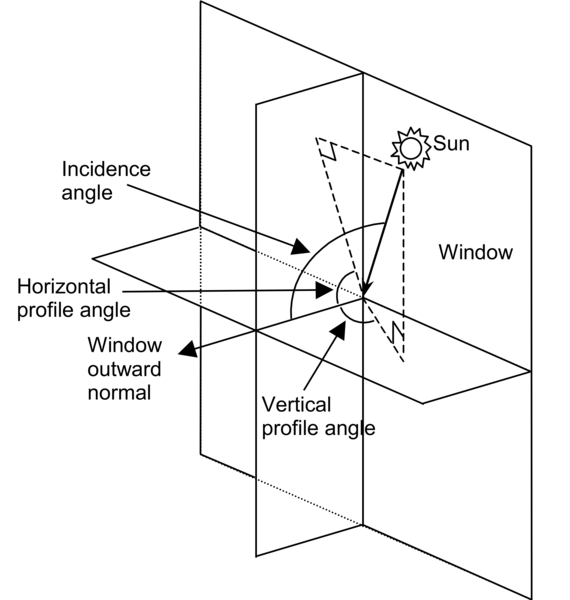
\includegraphics[width=0.9\textwidth, height=0.9\textheight, keepaspectratio=true]{media/image058.png}
\caption{Vertical exterior window showing solar horizontal profile angle, solar vertical profile angle and solar incidence angle. \protect \label{fig:vertical-exterior-window-showing-solar}}
\end{figure}

\subsubsection{Surface Window Outside Reveal Reflected Beam Solar Radiation Rate {[}W{]}}\label{surface-window-outside-reveal-reflected-beam-solar-radiation-rate-w}

\subsubsection{Surface Window Outside Reveal Reflected Beam Solar Radiation Energy {[}J{]}}\label{surface-window-outside-reveal-reflected-beam-solar-radiation-energy-j}

Beam solar radiation reflected from the outside reveal surfaces of a window (ref: Reveal Surfaces under WindowProperty:FrameAndDivider object). There are both rate and energy versions.

\subsubsection{Surface Window Inside Reveal Reflected Beam Solar Radiation Rate {[}W{]}}\label{surface-window-inside-reveal-reflected-beam-solar-radiation-rate-w}

\subsubsection{Surface Window Inside Reveal Reflected Beam Solar Radiation Energy {[}J{]}}\label{surface-window-inside-reveal-reflected-beam-solar-radiation-energy-j}

Beam solar radiation reflected from the inside reveal surfaces of a window (ref: Reveal Surfaces under WindowProperty:FrameAndDivider object). There are both rate and energy versions.

\subsubsection{Surface Window Inside Reveal Absorbed Beam Solar Radiation Rate {[}W{]}}\label{surface-window-inside-reveal-absorbed-beam-solar-radiation-rate-w}

Beam solar radiation absorbed at the inside reveal surfaces of a window, in Watts.

\subsubsection{Surface Window Inside Reveal Reflected Diffuse Zone Solar Radiation Rate {[}W{]}}\label{surface-window-inside-reveal-reflected-diffuse-zone-solar-radiation-rate-w}

Diffuse solar radiation reflected from inside reveal surfaces of a window into the zone, in Watts.

\subsubsection{Surface Window Inside Reveal Reflected Diffuse Frame Solar Radiation Rate {[}W{]}}\label{surface-window-inside-reveal-reflected-diffuse-frame-solar-radiation-rate-w}

Diffuse solar radiation reflected from inside reveal surfaces onto the frame surfaces of a window, in Watts.

\subsubsection{Surface Window Inside Reveal Reflected Diffuse Glazing Solar Radiation Rate {[}W{]}}\label{surface-window-inside-reveal-reflected-diffuse-glazing-solar-radiation-rate-w}

Diffuse solar radiation reflected from inside reveal surfaces onto the glazing surfaces of a window, in Watts.

\subsubsection{Surface Window Inside Face Glazing Condensation Status {[]}}\label{surface-window-inside-face-glazing-condensation-status}

A value of 1 means that moisture condensation will occur on the innermost glass face of an exterior window (i.e., on the glass face in contact with the zone air). Otherwise the value is 0. The condition for condensation is glass inside face temperature \textless{} zone air dewpoint temperature.

For airflow exterior windows, in which forced air passes between adjacent glass faces in double- and triple-pane windows, a value of 1 means that condensation will occur on one or both of the glass faces in contact with the airflow. In this case the condition for condensation is:

\begin{itemize}
\item
  \emph{For airflow source = indoorair}, temperature of either face in contact with airflow \textless{} zone air dewpoint temperature.
\item
  \emph{For airflow source = outdoorair}, temperature of either face in contact with airflow \textless{} outside air dewpoint temperature.
\end{itemize}

As for regular windows, the value will also be 1 if condensation occurs on the innermost glass face.

\subsubsection{Surface Window Inside Face Frame Condensation Status {[]}}\label{surface-window-inside-face-frame-condensation-status}

If an exterior window has a frame and the value of this flag is 1, condensation will occur on the inside surface of the frame. The condition for condensation is frame inside surface temperature \textless{} zone air dewpoint temperature.

\subsubsection{Surface Window Inside Face Divider Condensation Status {[]}}\label{surface-window-inside-face-divider-condensation-status}

If an exterior window has a divider and the value of this flag is 1, condensation will occur on the inside surface of the divider. The condition for condensation is divider inside surface temperature \textless{} zone air dewpoint temperature.

\subsubsection{Surface Shading Device Is On Time Fraction {[]}}\label{surface-shading-device-is-on-time-fraction}

The fraction of time that a shading device is on an exterior window. For a particular simulation timestep, the value is 0.0 if the shading device is off (or there is no shading device) and the value is 1.0 if the shading device is on. (It is assumed that the shading device, if present, is either on or off for the entire timestep.) If the shading device is switchable glazing, a value of 0.0 means that the glazing is in the unswitched (light colored) state, and a value of 1.0 means that the glazing is in the switched (dark colored) state.

For a time interval longer a timestep, this is the fraction of the time interval that the shading device is on. For example, take the case where the time interval is one hour and the timestep is 10 minutes. Then if the shading device is on for two timesteps in the hour and off for the other four timesteps, then the fraction of time that the shading device is on = 2/6 = 0.3333.

\subsubsection{Surface Window Blind Slat Angle {[}deg{]}}\label{surface-window-blind-slat-angle-deg}

For an exterior window with a blind, this is the angle in degrees between the glazing outward normal and the blind slat angle outward normal, where the outward normal points away from the front face of the slat. The slat angle varies from 0 to 180 deg. If the slat angle is 0 deg or 180 deg, the slats are parallel to the glazing and the slats are said to be ``closed''. If the slat angle is 90 deg, the slats are perpendicular to the glazing and the slats are said to be ``fully open''. See illustrations under WindowMaterial:Blind. For blinds with a fixed slat angle, the value reported here will be constant.

For WindowMaterial:Blind:EquivalentLayer blinds the slat angle varies from -90 to 90 deg. If the slat angle is -90 deg or 90 deg, the slats are parallel to the glazing and the slats are said to be ``closed''. If the slat angle is 0 deg, the slats are perpendicular to the glazing and the slats are said to be ``fully open''. For blinds with a fixed slat angle, the value reported here will be constant.


\subsubsection{Surface Window Blind Beam to Beam Solar Transmittance {[]}}\label{surface-window-blind-beam-to-beam-solar-transmittance}

For an exterior window with a blind, this is the fraction of exterior beam solar radiation incident on the blind that is transmitted through the blind as beam solar radiation when the blind is isolated (i.e., as though the window glass were not present). Depends on various factors, including slat angle, width, separation, and thickness, and horizontal solar profile angle (for blinds with horizontal slats) or vertical solar profile angle (for blinds with vertical slats). The transmittance value reported here will be non-zero only when some beam solar can pass through the blind without hitting the slats.

\subsubsection{Surface Window Blind Beam to Diffuse Solar Transmittance {[]}}\label{surface-window-blind-beam-to-diffuse-solar-transmittance}

For an exterior window with a blind, the fraction of exterior beam solar radiation incident on the blind that is transmitted through the blind as diffuse solar radiation when the blind is isolated (i.e., as though the window glass were not present). Depends on various factors, including slat angle, width, separation, thickness and reflectance, and horizontal solar profile angle (for blinds with horizontal slats) or vertical solar profile angle (for blinds with vertical slats).

\subsubsection{Surface Window Blind Diffuse to Diffuse Solar Transmittance {[]}}\label{surface-window-blind-diffuse-to-diffuse-solar-transmittance}

For an exterior window with a blind, the fraction of exterior diffuse solar radiation incident on the blind that is transmitted through the blind as diffuse solar radiation when the blind is isolated (i.e., as though the window glass were not present). Depends on various factors, including slat angle, width, separation, thickness and reflectance. For blinds with a fixed slat angle the transmittance value reported here will be constant.

\subsubsection{Surface Window Blind and Glazing System Beam Solar Transmittance {[]}}\label{surface-window-blind-and-glazing-system-beam-solar-transmittance}

The fraction of exterior beam solar radiation incident on an exterior window with a blind (excluding window frame, if present) that is transmitted through the blind/glass system as beam solar radiation. Depends on various factors, including type of glass; solar incidence angle; slat angle, width, separation, and thickness; and horizontal solar profile angle (for blinds with horizontal slats) or vertical solar profile angle (for blinds with vertical slats).

\subsubsection{Surface Window Blind and Glazing System Diffuse Solar Transmittance {[]}}\label{surface-window-blind-and-glazing-system-diffuse-solar-transmittance}

The fraction of exterior diffuse solar radiation incident on an exterior window with a blind (excluding window frame, if present) that is transmitted through the blind/glass system as diffuse solar radiation. Depends on various factors, including type of glass and slat angle, width, separation, thickness and reflectance. For blinds with a fixed slat angle the transmittance value reported here will be constant.

\subsubsection{Surface Window Screen Beam to Beam Solar Transmittance {[]}}\label{surface-window-screen-beam-to-beam-solar-transmittance}

For an exterior window with a screen, this is the fraction of exterior beam solar radiation incident on the screen that is transmitted through the screen as beam solar radiation when the screen is isolated (i.e., as though the window glass were not present). Depends on various factors, including the screen reflectance and the relative angle of the incident beam with respect to the screen. This value will include the amount of inward reflection of solar beam off the screen material surface if the user specifies this modeling option (i.e., Material: WindowScreen, field Reflected Beam Transmittance Accounting Method = Model as Direct Beam).

\subsubsection{Surface Window Screen Beam to Diffuse Solar Transmittance{[]}}\label{surface-window-screen-beam-to-diffuse-solar-transmittance}

For an exterior window with a screen, the fraction of exterior beam solar radiation incident on the screen that is transmitted through the screen as diffuse solar radiation when the screen is isolated (i.e., as though the window glass were not present). Depends on various factors, including the screen reflectance and the relative angle of the incident beam with respect to the screen. This value is the amount of inward reflection of solar beam off the screen material surface if the user specifies this modeling option (i.e., Material: WindowScreen, field Reflected Beam Transmittance Accounting Method = Model as Diffuse); otherwise, this value will be zero.

\subsubsection{Surface Window Screen Diffuse to Diffuse Solar Transmittance{[]}}\label{surface-window-screen-diffuse-to-diffuse-solar-transmittance}

For an exterior window with a screen, the fraction of exterior diffuse solar radiation incident on the screen that is transmitted through the screen as diffuse solar radiation when the screen is isolated (i.e., as though the window glass were not present). Depends on various factors including screen material geometry and reflectance. This value is calculated as an average, constant For a window with a screen, this value consists of diffuse radiation transmitted through the screen (gaps between the screen material) and diffuse radiation from diffuse-to-diffuse reflection from the screen material. For a window with a screen, this value consists of diffuse radiation transmitted through the screen (gaps between the screen material) and diffuse radiation from diffuse-to-diffuse reflection from the screen material.

\subsubsection{Surface Window Screen and Glazing System Beam Solar Transmittance{[]}}\label{surface-window-screen-and-glazing-system-beam-solar-transmittance}

The fraction of exterior beam solar radiation incident on an exterior window with a screen (excluding window frame, if present) that is transmitted through the screen/glass system as beam solar radiation. Depends on various factors, including the screen reflectance and the relative angle of the incident beam with respect to the screen. This value will include the amount of inward reflection of solar beam off the screen material surface if the user specifies this modeling option (i.e., Material: WindowScreen, field Reflected Beam Transmittance Accounting Method = Model as Direct Beam).

\subsubsection{Surface Window Screen and Glazing System Diffuse Solar Transmittance {[]}}\label{surface-window-screen-and-glazing-system-diffuse-solar-transmittance}

The fraction of exterior diffuse solar radiation incident on an exterior window with a screen (excluding window frame, if present) that is transmitted through the screen/glass system as diffuse solar radiation. Depends on various factors including screen material geometry and reflectance.

\subsubsection{Surface Window Transmitted Beam Solar Radiation Rate {[}W{]}}\label{surface-window-transmitted-beam-solar-radiation-rate-w-1}

\subsubsection{Surface Window Transmitted Beam Solar Radiation Energy {[}J{]}}\label{surface-window-transmitted-beam-solar-radiation-energy-j-1}

The beam solar radiation transmitted through an interior window. Calculated only if Solar Distribution = FullInteriorAndExterior in your Building input. The origin of this radiation is beam solar that enters through an exterior window in a zone and then passes through an interior window into the adjacent zone. The amount of this radiation depends on several factors, including sun position, intensity of beam solar incident on the exterior window (including effects of shadowing, if present), relative position of the exterior and interior window, and the size and transmittance of the windows. Note that if there are two or more exterior windows in a zone, then beam solar from one or more of them may pass through the same interior window. Likewise, if there are more than two or more interior windows in a zone then beam solar from a single exterior window may pass through one or more of the interior windows. There are both rate and energy versions of the output.

\subsubsection{Surface Storm Window On Off Status {[]}}\label{surface-storm-window-on-off-status}

Indicates whether a storm window glass layer is present (ref: StormWindow object). The value is \textbf{0} if the storm window glass layer is off, \textbf{1} if it is on, and \textbf{--1} if the window does not have an associated storm window. Applicable only to exterior windows and glass doors.

\subsubsection{Surface Inside Face Initial Transmitted Diffuse Transmitted Out Window Solar Radiation Rate {[}W{]}}\label{surface-inside-face-initial-transmitted-diffuse-transmitted-out-window-solar-radiation-rate-w}

As of Version 2.1, the diffuse solar transmitted through exterior windows that is initially distributed to another window in the zone and transmitted out of the zone through that window. For exterior windows, this transmitted diffuse solar is ``lost'' to the exterior environment For interior windows, this transmitted diffuse solar is distributed to heat transfer surfaces in the adjacent zone, and is part of the Surface Inside Face Initial Transmitted Diffuse Absorbed Solar Radiation Rate for these adjacent zone surfaces.

\subsubsection{Additional Window Outputs (Advanced)}\label{additional-window-outputs-advanced}

The following output variables for windows or glass doors are available when the user requests to display advanced output variables. These seven reports show the individual components that are combined to determine overall Surface Window Heat Gain Rate and/or Surface Window Heat Loss Rate (described above).

\subsubsection{Surface Window Inside Face Glazing Zone Convection Heat Gain Rate {[}W{]}}\label{surface-window-inside-face-glazing-zone-convection-heat-gain-rate-w}

The surface convection heat transfer from the glazing to the zone in watts. This output variable is the term called ``{[}Convective heat flow to the zone from the zone side of the glazing{]}'' under the description above for Surface Window Heat Gain Rate output variable. If the window has an interior shade or blind, then this is zero and the glazing's convection is included in the report called ``Surface Window Inside Face Gap between Shade and Glazing Zone Convection Heat Gain Rate''.

\subsubsection{Surface Window Inside Face Glazing Net Infrared Heat Transfer Rate {[}W{]}}\label{surface-window-inside-face-glazing-net-infrared-heat-transfer-rate-w}

The net exchange of infrared radiation heat transfer from the glazing to the zone in watts. This output variable is the term called ``{[}Net IR heat flow to the zone from zone side of the glazing{]}'' under the description above for Surface Window Heat Gain Rate output variable.

\subsubsection{Surface Window Shortwave from Zone Back Out Window Heat Transfer Rate {[}W{]}}\label{surface-window-shortwave-from-zone-back-out-window-heat-transfer-rate-w}

This is the short-wave radiation heat transfer from the zone back out the window in watts. This is a measure of the diffuse short-wave light (from reflected solar and electric lighting) that leave the zone through the window. This output variable is the term called ``{[}Short-wave radiation from zone transmitted back out the window{]}'' under the description above for Surface Window Heat Gain Rate output variable.

\subsubsection{Surface Window Inside Face Frame and Divider Zone Heat Gain Rate {[}W{]}}\label{surface-window-inside-face-frame-and-divider-zone-heat-gain-rate-w}

This is the heat transfer from any frames and/or dividers to the zone in watts. This output variable is the term called ``{[}Conduction to zone from window frame and divider, if present{]}'' under the description above for Surface Window Heat Gain Rate output variable. (The word ``conduction'' here is used because the models is simplified compared to the complexities of surface convection and radiation.)

\subsubsection{Surface Window Frame Heat Gain Rate {[}W{]}}\label{surface-window-frame-heat-gain-rate-w}

This is the positive heat flow from window frames to the zone in watts. This is part of the Surface Window Inside Face Frame and Divider Zone Heat Gain Rate.

\subsubsection{Surface Window Frame Heat Loss Rate {[}W{]}}\label{surface-window-frame-heat-loss-rate-w}

This is the negative heat flow from window frames to the zone in watts. This is part of the Surface Window Inside Face Frame and Divider Zone Heat Gain Rate.

\subsubsection{Surface Window Frame Inside Temperature {[}C{]}}\label{surface-window-frame-inside-temperature-c}

This is the temperature of the inside surface of the window frames.

\subsubsection{Surface Window Frame Outside Temperature {[}C{]}}\label{surface-window-frame-outside-temperature-c}

This is the temperature of the outside surface of the window frames.

\subsubsection{Surface Window Divider Heat Gain Rate {[}W{]}}\label{surface-window-divider-heat-gain-rate-w}

This is the positive heat flow from window dividers to the zone in watts. This is part of the Surface Window Inside Face Frame and Divider Zone Heat Gain Rate.

\subsubsection{Surface Window Divider Heat Loss Rate {[}W{]}}\label{surface-window-divider-heat-loss-rate-w}

This is the negative heat flow from window dividers to the zone in watts. This is part of the Surface Window Inside Face Frame and Divider Zone Heat Gain Rate.

\subsubsection{Surface Window Divider Inside Temperature {[}C{]}}\label{surface-window-divider-inside-temperature-c}

This is the temperature of the inside surface of the window dividers.

\subsubsection{Surface Window Divider Outside Temperature {[}C{]}}\label{surface-window-divider-outside-temperature-c}

This is the temperature of the outside surface of the window dividers.

\subsubsection{Surface Window Inside Face Gap between Shade and Glazing Zone Convection Heat Gain Rate {[}W{]}}\label{surface-window-inside-face-gap-between-shade-and-glazing-zone-convection-heat-gain-rate-w}

This is the convection surface heat transfer from the both the glazing and the shade's back face to the zone in Watts. This output variable is the term called ``{[}Convective heat flow to the zone from the air flowing through the gap between glazing and shading device{]}'' under the description above for Surface Window Heat Gain Rate output variable. For Equivalent Layer window this output variable is the convection heat gain from vented interior air gap to the zone in Watts.

\subsubsection{Surface Window Inside Face Shade Zone Convection Heat Gain Rate {[}W{]}}\label{surface-window-inside-face-shade-zone-convection-heat-gain-rate-w}

This is the convection surface heat transfer from the front side of any interior shade or blind to the zone in Watts. This output variable is the term called ``{[}Convective heat flow to the zone from the zone side of the shading device{]}'' under the description above for Surface Window Heat Gain Rate output variable. For equivalent Layer window this output variable is the convection heat gain rate from the inside face of a glazing or a shade to the zone in Watts.

\subsubsection{Surface Window Inside Face Shade Net Infrared Heat Transfer Rate {[}W{]}}\label{surface-window-inside-face-shade-net-infrared-heat-transfer-rate-w}

The net exchange of infrared radiation heat transfer from the shade or blind to the zone in watts. This output variable is the term called ``{[}Net IR heat flow to the zone from the zone side of the shading device{]}'' under the description above for Surface Window Heat Gain Rate output variable.

\subsubsection{Surface Window Inside Face Other Convection Heat Gain Rate {[}W{]}}\label{surface-window-inside-face-other-convection-heat-gain-rate-w}

The other (extra) convection heat transfer rate from the inside face of a an equivalent layer window. This output is computed from the difference in convection flux when using equivalent inside surface temperature of a window instead of the inside surface temperature from the standard surface heat balance calculation.

\subsection{Thermochromic Window Outputs}\label{thermochomic-window-outputs}

\subsubsection{Window Thermochromic Layer Temperature {[}C{]}}\label{window-thermochromic-layer-temperature-c}

The temperature of the TC glass layer of a TC window at each time step.

\subsubsection{Surface Window Thermochromic Layer Property Specification Temperature {[}C{]}}\label{surface-window-thermochromic-layer-property-specification-temperature-c-000}

The temperature under which the optical data of the TC glass layer are specified.

The overall properties (U-factor/SHGC/VT) of the thermochromic windows at different specification temperatures are reported in the \textbf{.eio} file. These window constructions are created by EnergyPlus during run time. They have similar names with suffix ``\_TC\_XX'' where XX represents a specification temperature.

\subsubsection{Switchable Window Outputs}\label{switchable-window-outputs}

\subsubsection{Surface Window Switchable Glazing Switching Factor{[]}}\label{surface-window-switchable-glazing-switching-factor}

The switching factor (tint level) of the switchable window: 0 means no switching -- clear state; 1 means fully switched -- dark state.

\subsubsection{Surface Window Switchable Glazing Visible Transmittance{[]}}\label{surface-window-switchable-glazing-visible-transmittance}

The visible transmittance of the switchable window.

\subsection{Other Surface Outputs/Reports}\label{other-surface-outputsreports}

Several reports can be selected for Surfaces. (See Group -- Report for details on how to specify). Examples are:

\subsubsection{DXF}\label{dxf}

This report produces a special file (\textbf{eplusout.dxf}) in the industry standard DXF (Drawing Interchange Format) for drawings. It is produced and accepted by many popular, commercial CAD programs. Detailed reference can be found on the AutoCAD™ website at: \url{http://www.autodesk.com/techpubs/autocad/acadr14/dxf/index.htm}.

EnergyPlus produces this file from the Report command:

\begin{lstlisting}

Output:Reports, Surfaces, DXF;
\end{lstlisting}

\subsubsection{Details, Vertices, DetailsWithVertices}\label{details-vertices-detailswithvertices}

This version of the report creates lines in the eplusout.eio file for each surface (except internal mass surfaces). Details of this reporting is shown in the Output Details and Examples document.

\subsection{Shading Surfaces}\label{shading-surfaces}

Shading surfaces are entities outside of the building that may cast shadows on the building's heat transfer surfaces. These entities do not typically have enough thermal mass to be described as part of the building's thermal makeup.

The most important effect of shading surfaces is to reduce solar gain in windows that are shadowed. (However, in some cases, shading surfaces can reflect solar onto a wall or window and increase solar gain.)

There are two kinds of shading surfaces in EnergyPlus: \textbf{detached} and \textbf{attached}. A \textbf{detached} shading surface, such as a tree or neighboring building, is not connected to the building. An \textbf{attached} shading surface is typically an overhang or fin that is attached to a particular base surface of the building, usually a wall; attached shading surfaces are usually designed to shade specific windows.

Objects for detached shading surfaces:

\begin{itemize}
\item
  Shading:Site
\item
  Shading:Building
\item
  Shading:Site:Detailed
\item
  Shading:Building:Detailed
\end{itemize}

Similarly to the surfaces, the detailed objects use vertex entry whereas the other objects are limited to rectangular representation.

Objects for attached shading surfaces:

\begin{itemize}
\item
  Shading:Overhang
\item
  Shading:Overhang:Projection
\item
  Shading:Fin
\item
  Shading:Fin:Projection
\item
  Shading:Zone:Detailed
\end{itemize}

EnergyPlus creates ``bi-directional'' shades from each shading surface entered. This means that the shade you input will cast a shadow no matter which side of the shade the sun is on. For example, a vertical fin will cast a shadow whether the sun is on the left side or right side of the fin. Prior to V1.0.2, a shading surface cast a shadow only in the hemisphere toward which the surface faced. This hemisphere is the one pointed to by the shading surface's outward normal vector, which is the cross product V23 x V21, where V23 is the vector from vertex 2 to vertex 3 of the shading surface and V21 is the vector from vertex 2 to vertex 1. Beginning with V1.0.2, the shades in EnergyPlus are ``bi-directional'' so that they can cast shadows in both hemispheres depending on the time-varying position of the sun relative to the shading surface.

It is important to note that EnergyPlus will automatically account for ``self-shading'' effects---such as in L-shaped buildings---in which some of the building's wall and roof surfaces shade other parts of the building, especially windows. This means that you only need to describe shading elements that aren't building heat-transfer surfaces.

Shading surfaces can also \textbf{reflect} solar radiation onto the building. This feature is simulated if you choose FullExteriorWithReflections or FullInteriorAndExteriorWithReflections in the Building object (ref: Building - Field: Solar Distribution). In this case, you may specify the reflectance properties of a shading surface with the ShadingProperty:Reflectance object. Note: If no ShadingProperty:Reflectance object is defined, then the shading surface reflectance values are assumed to be 0.2 and the fraction of shading surface that is glazed is assumed to be 0.0.

Shading surfaces also automatically shade diffuse solar radiation (and long-wave radiation) from the sky. And they will automatically shade diffuse solar radiation from the ground if Solar Distribution Field = FullExteriorWithReflections or FullInteriorAndExteriorWithReflections in the Building object. (If the reflections option for Solar Distribution is used, the program also takes into account the reduction of solar radiation reflected from the ground due to shading of the ground by shading surfaces and by the building itself.) Otherwise, shading surfaces will not shade diffuse radiation from the ground unless you enter a reduced value for View Factor to Ground for those building surfaces that are shaded (ref: BuildingSurface:Detailed - Field: View Factor to Ground and FenestrationSurface:Detailed - Field: View Factor to Ground).

\subsection{Detached Shading Surfaces}\label{detached-shading-surfaces}

\subsection{Shading:Site, Shading:Building}\label{shadingsite-shadingbuilding}

These objects are used to describe rectangular shading elements that are external to the building. Examples are trees, high fences, near-by hills, and neighboring buildings.

If relative coordinates are used (ref: Field: Coordinate System in GlobalGeometryRules), shading surfaces entered with Shading:Site remain stationary if the building is rotated, whereas those entered with Shading:Building rotate with the building. If world coordinates are used Shading:Site and Shading:Building are equivalent.

These shading elements are always opaque.

\subsubsection{Field: Name}\label{field-name-22-004}

This is a unique character string associated with the detached shading surface. Though it must be unique from other surface names, it is used primarily for convenience with detached shading surfaces.

\subsubsection{Field: Azimuth Angle}\label{field-azimuth-angle-10}

Theoretically, this should face to the surface it is shading (i.e.~if a south wall, this should be a north facing shade) but since EnergyPlus automatically generates the mirror image, the facing angle per se' is not so important.

\subsubsection{Field: Tilt Angle}\label{field-tilt-angle-10}

The tilt angle is the angle (in degrees) that the shade is tilted from horizontal (or the ground). Default for this field is 90 degrees.

\subsubsection{Starting Corner for the surface}\label{starting-corner-for-the-surface-16}

The rectangular surfaces specify the lower left corner of the surface for their starting coordinate. See the introductory paragraph for rules on this entry.

\subsubsection{Field: Starting X Coordinate}\label{field-starting-x-coordinate-16}

This field is the X coordinate (in meters).

\subsubsection{Field: Starting Y Coordinate}\label{field-starting-y-coordinate-10}

This field is the Y coordinate (in meters).

\subsubsection{Field: Starting Z Coordinate}\label{field-starting-z-coordinate-16}

This field is the Z coordinate (in meters).

\subsubsection{Field: Length}\label{field-length-16}

This field is the length of the shade in meters.

\subsubsection{Field: Height}\label{field-height-10}

This field is the width of the shade in meters.

Examples of these (can be found in example files 4ZoneWithShading\_Simple\_1.idf and 4ZoneWithShading\_Simple\_2.idf)

\begin{lstlisting}

  Shading:Building,
      Bushes-East,             !- Name
      90,                      !- Azimuth Angle {deg}
      90,                      !- Tilt Angle {deg}
      45,                      !- Starting X Coordinate {m}
      0,                       !- Starting Y Coordinate {m}
      0,                       !- Starting Z Coordinate {m}
      50,                      !- Length {m}
      1;                       !- Height {m}

    Shading:Site,
      Bushes-North,            !- Name
      0,                       !- Azimuth Angle {deg}
      90,                      !- Tilt Angle {deg}
      45,                      !- Starting X Coordinate {m}
      50,                      !- Starting Y Coordinate {m}
      0,                       !- Starting Z Coordinate {m}
      50,                      !- Length {m}
      1;                       !- Height {m}
\end{lstlisting}

\subsection{Shading:Site:Detailed, Shading:Building:Detailed}\label{shadingsitedetailed-shadingbuildingdetailed}

These objects are used to describe shading elements that are external to the building. Examples are trees, high fences, near-by hills, and neighboring buildings.

If relative coordinates are used (ref: Field: Coordinate System in GlobalGeometryRules), shading surfaces entered with Shading:Site:Detailed remain stationary if the building is rotated, whereas those entered with Shading:Building:Detailed rotate with the building. If world coordinates are used Shading:Site:Detailed and Shading:Building:Detailed are equivalent.

While ``detached'' implies that shading surfaces are not part of the building, the detached shading sequence can be used to describe attached shading surfaces that may shade heat transfer surfaces in more than one zone. For example, wing A of a building might shade several zones of wing B but wing A (for whatever reason) is not described in the geometry for the simulation so it is represented by a detached shade to get its shadowing effect.

\subsubsection{Field: Name}\label{field-name-23-004}

This is a unique character string associated with the detached shading surface. Though it must be unique from other surface names, it is used primarily for convenience with detached shading surfaces.

\subsubsection{Field: Transmittance Schedule Name}\label{field-transmittance-schedule-name}

The name of a schedule of solar transmittance values from 0.0 to 1.0 for the shading surface. If a blank is entered in this field, the transmittance value defaults to 0.0, i.e., the shading surface is opaque at all times. This scheduling can be used to allow for seasonal transmittance change, such as for deciduous trees that have a higher transmittance in winter than in summer. Transmittance based on time of day can also be used---a movable awning, for example, where the transmittance is some value less than 1.0 when the awning is in place and is 1.0 when the awning is retracted.

The following assumptions are made in the shading surface transmittance calculation:

\begin{itemize}
\item
  Both sides of the shading surface have the same transmittance properties.
\item
  The transmittance is the same for both beam and diffuse solar radiation.
\item
  Beam solar transmittance is independent of angle of incidence on the shading surface.
\item
  Beam radiation incident on a shading surface is transmitted as beam radiation with no change in direction, i.e., there is no beam-to-diffuse component.
\item
  If two shading surfaces with non-zero transmittance overlap, the net transmittance is the product of the individual transmittances. Inter-reflection between the shading surfaces (and between the shading surfaces and the building) is ignored.
\item
  For the daylighting calculation (ref: Group -- Daylighting) the shading surface's visible transmittance is assumed to be the same as its solar transmittance.
\item
  Shading devices are assumed to be opaque to long-wave radiation no matter what the solar transmittance value is.
\end{itemize}

Note that shading devices only shade solar radiation when the sun is up, which is automatically determined by EnergyPlus from latitude, time of year, etc. The user need only account for the time-varying transmittance of the shading device in the transmittance schedule, not whether the sun is up or not.

\subsubsection{Field: Number Vertices}\label{field-number-vertices}

The number of sides in the surface (number of X,Y,Z vertex groups). For further information, see the discussion on ``Surface Vertices'' above.

IDF example of Detached Shading Surfaces:

\begin{lstlisting}

Shading:Building:Detailed,
     EAST SIDE TREE,  !- Detached Shading
     ShadingTransmittance:0002,  !- Shadowing Transmittance & Schedule
     3, !-Triangle
     33.52800    ,   10.66800    ,   10.05800    ,
     33.52800    ,   13.71600    ,  0.9140000    ,
     33.52800    ,   4.572000    ,  0.9140000    ;

  Shading:Building:Detailed,
     WEST SIDE TREE,  !- Detached Shading
     ShadingTransmittance:0002,  !- Shadowing Transmittance & Schedule
     3, !-Triangle
    -3.048000    ,   7.620000    ,   10.05800    ,
    -3.048000    ,   4.572000    ,  0.9140000    ,
    -3.048000    ,   13.71600    ,  0.9140000    ;
\end{lstlisting}

\subsection{Attached Shading Surfaces}\label{attached-shading-surfaces}

Overhangs are usually horizontal devices that are used to shade windows. Fins are usually vertical devices that similarly shade windows.

\subsection{Shading:Overhang}\label{shadingoverhang}

An overhang typically is used to shade a window in a building.

\subsubsection{Inputs}\label{inputs-26-003}

\paragraph{Field: Name}\label{field-name-24-003}

This is the name of the overhang. It must be different from other surface names.

\paragraph{Field: Window or Door Name}\label{field-window-or-door-name}

The name of a window or door that this overhang shades.

\paragraph{Field: Height above Window or Door}\label{field-height-above-window-or-door}

This field is the height (meters) above the top of the door for the overhang.

\paragraph{Field Tilt Angle from Window/Door}\label{field-tilt-angle-from-windowdoor}

This field is the tilt angle from the Window/Door. For a flat overhang, this would be 90 (degrees).

\paragraph{Field: Left Extension from Window/Door Width}\label{field-left-extension-from-windowdoor-width}

This field is the width from the left edge of the window/door to the start of the overhang (meters).

\paragraph{Field: Right Extension from Window/Door Width}\label{field-right-extension-from-windowdoor-width}

This field is the width from the right edge of the window/door to the start of the overhang (meters).

\paragraph{Field: Depth}\label{field-depth}

This field is the depth of the overhang (meters) projecting out from the wall.

\subsection{Shading:Overhang:Projection}\label{shadingoverhangprojection}

An overhang typically is used to shade a window in a building. This object allows for specifying the depth of the overhang as a fraction of the window or door's height.

\subsubsection{Inputs}\label{inputs-27-003}

\paragraph{Field: Name}\label{field-name-25-003}

This is the name of the overhang. It must be different from other surface names.

\paragraph{Field: Window or Door Name}\label{field-window-or-door-name-1}

The name of a window or door that this overhang shades.

\paragraph{Field: Height above Window or Door}\label{field-height-above-window-or-door-1}

This field is the height (meters) above the top of the door for the overhang.

\paragraph{Field Tilt Angle from Window/Door}\label{field-tilt-angle-from-windowdoor-1}

This field is the tilt angle from the Window/Door. For a flat overhang, this would be 90 (degrees).

\paragraph{Field: Left Extension from Window/Door Width}\label{field-left-extension-from-windowdoor-width-1}

This field is the width from the left edge of the window/door to the start of the overhang (meters).

\paragraph{Field: Right Extension from Window/Door Width}\label{field-right-extension-from-windowdoor-width-1}

This field is the width from the right edge of the window/door to the start of the overhang (meters).

\paragraph{Field: Depth as Fraction of Window/Door Height}\label{field-depth-as-fraction-of-windowdoor-height}

This field is the fraction of the window/door height to specify as the depth of the overhang (meters) projecting out from the wall.

\subsection{Shading:Fin}\label{shadingfin}

Fins shade either side of windows/doors in a building. This object allows for specification of both fins for the window. Fin placement is relative to the edge of the glass and user must include the frame width when a frame is present.

\subsubsection{Inputs}\label{inputs-28-002}

\paragraph{Field: Name}\label{field-name-26-003}

This is the name of the overhang. It must be different from other surface names.

\paragraph{Field: Window or Door Name}\label{field-window-or-door-name-2}

The name of a window or door that this overhang shades.

\paragraph{Field: Left Fin Extension from Window/Door}\label{field-left-fin-extension-from-windowdoor}

This field is the width from the left edge of the window/door to the plane of the left fin (meters). The extension width is relative to the edge of the glass and includes the frame width when a frame is present.

\paragraph{Field: Left Fin Distance Above Top of Window}\label{field-left-fin-distance-above-top-of-window}

This field is the distance from the top of the window to the top of the left fin (meters) and is relative to the edge of the glass and includes the frame width when a frame is present.

\paragraph{Field: Left Fin Distance Below Bottom of Window}\label{field-left-fin-distance-below-bottom-of-window}

This field is the distance from the bottom of the window to the bottom of the left fin (meters) and is relative to the edge of the glass and includes the frame width when a frame is present.

\paragraph{Field: Left Fin Tilt Angle from Window/Door}\label{field-left-fin-tilt-angle-from-windowdoor}

This field is the tilt angle from the window / door for the left fin. Typically, a fin is 90 degrees (default) from its associated window/door.

\paragraph{Field: Left Fin Depth}\label{field-left-fin-depth}

This field is the depth (meters) of the left fin (projecting out from the wall).

\paragraph{Field: Right Fin Extension from Window/Door}\label{field-right-fin-extension-from-windowdoor}

This field is the width from the right edge of the window/door to the plane of the right fin (meters). The extension width is relative to the edge of the glass and includes the frame width when a frame is present.

\paragraph{Field: Right Fin Distance Above Top of Window}\label{field-right-fin-distance-above-top-of-window}

This field is the distance from the top of the window to the top of the right fin (meters) and is relative to the edge of the glass and includes the frame width when a frame is present.

\paragraph{Field: Right Fin Distance Below Bottom of Window}\label{field-right-fin-distance-below-bottom-of-window}

This field is the distance from the bottom of the window to the bottom of the right fin (meters) and is relative to the edge of the glass and includes the frame width.

\paragraph{Field: Right Fin Tilt Angle from Window/Door}\label{field-right-fin-tilt-angle-from-windowdoor}

This field is the tilt angle from the window / door for the right fin. Typically, a fin is 90 degrees (default) from its associated window/door.

\paragraph{Field: Right Fin Depth}\label{field-right-fin-depth}

This field is the depth (meters) of the right fin (projecting out from the wall).

\subsection{Shading:Fin:Projection}\label{shadingfinprojection}

Fins shade either side of windows/doors in a building. This object allows for specification of both fins for the window. This object allows for specifying the depth of the overhang as a fraction of the window or door's width. Fin placement is relative to the edge of the glass and user must include the frame width when a frame is present.

\subsubsection{Inputs}\label{inputs-29-002}

\paragraph{Field: Name}\label{field-name-27-003}

This is the name of the overhang. It must be different from other surface names.

\paragraph{Field: Window or Door Name}\label{field-window-or-door-name-3}

The name of a window or door that this overhang shades.

\paragraph{Field: Left Fin Extension from Window/Door}\label{field-left-fin-extension-from-windowdoor-1}

This field is the width from the left edge of the window/door to the plane of the left fin (meters). The extension width is relative to the edge of the glass and includes the frame width when a frame is present.

\paragraph{Field: Left Fin Distance Above Top of Window}\label{field-left-fin-distance-above-top-of-window-1}

This field is the distance from the top of the window to the top of the left fin (meters) and is relative to the edge of the glass and includes the frame width when a frame is present.

\paragraph{Field: Left Fin Distance Below Bottom of Window}\label{field-left-fin-distance-below-bottom-of-window-1}

This field is the distance from the bottom of the window to the bottom of the left fin (meters) and is relative to the edge of the glass and includes the frame width when a frame is present.

\paragraph{Field: Left Fin Tilt Angle from Window/Door}\label{field-left-fin-tilt-angle-from-windowdoor-1}

This field is the tilt angle from the window / door for the left fin. Typically, a fin is 90 degrees (default) from its associated window/door.

\paragraph{Field: Left Fin Depth as Fraction of Window/Door Width}\label{field-left-fin-depth-as-fraction-of-windowdoor-width}

This field is the fraction of the window/door width to specify as the depth of the left fin (meters) projecting out from the wall.

\paragraph{Field: Right Fin Extension from Window/Door}\label{field-right-fin-extension-from-windowdoor-1}

This field is the width from the right edge of the window/door to the plane of the right fin (meters).. The extension width is relative to the edge of the glass and includes the frame width when a frame is present.

\paragraph{Field: Right Fin Distance Above Top of Window}\label{field-right-fin-distance-above-top-of-window-1}

This field is the distance from the top of the window to the top of the right fin (meters) and is relative to the edge of the glass and includes the frame width when a frame is present.

\paragraph{Field: Right Fin Distance Below Bottom of Window}\label{field-right-fin-distance-below-bottom-of-window-1}

This field is the distance from the bottom of the window to the bottom of the right fin (meters) and is relative to the edge of the glass and includes the frame width when a frame is present.

\paragraph{Field: Right Fin Tilt Angle from Window/Door}\label{field-right-fin-tilt-angle-from-windowdoor-1}

This field is the tilt angle from the window / door for the right fin. Typically, a fin is 90 degrees (default) from its associated window/door.

\paragraph{Field: Right Fin Depth as Fraction of Window/Door Width}\label{field-right-fin-depth-as-fraction-of-windowdoor-width}

This field is the fraction of the window/door width to specify as the depth of the right fin (meters) projecting out from the wall.

zone.

Examples of these (can be found in example files 4ZoneWithShading\_Simple\_1.idf and 4ZoneWithShading\_Simple\_2.idf)

\begin{lstlisting}

  Shading:Overhang:Projection,
      Zn001:Wall001:Win001:Shade001,  !- Name
      Zn001:Wall001:Win001,    !- Window or Door Name
      .7,                      !- Height above Window or Door {m}
      90,                      !- Tilt Angle from Window/Door {deg}
      .2,                      !- Left extension from Window/Door Width {m}
      .2,                      !- Right extension from Window/Door Width {m}
      .6;                      !- Depth as Fraction of Window/Door Height {m}

    Shading:Overhang,
      Zn001:Wall001:Door001:Shade001,  !- Name
      Zn001:Wall001:Door001,   !- Window or Door Name
      .6,                      !- Height above Window or Door {m}
      90,                      !- Tilt Angle from Window/Door {deg}
      0,                       !- Left extension from Window/Door Width {m}
      0,                       !- Right extension from Window/Door Width {m}
      3;                       !- Depth {m}

    Shading:Fin:Projection,
      Zn001:Wall001:Shade003,  !- Name
      Zn001:Wall001:Win001,    !- Window or Door Name
      .1,                      !- Left Extension from Window/Door {m}
      .1,                   !- Left Distance Above Top of Window {m}
      .1,                   !- Left Distance Below Bottom of Window {m}
      90,                   !- Left Tilt Angle from Window/Door {deg}
      .6,                   !- Left Depth as Fraction of Window/Door Width {m}
      .1,                   !- Right Extension from Window/Door {m}
      .1,                   !- Right Distance Above Top of Window {m}
      .1,                   !- Right Distance Below Bottom of Window {m}
      90,                   !- Right Tilt Angle from Window/Door {deg}
      .6;                   !- Right Depth as Fraction of Window/Door Width {m}
\end{lstlisting}

\subsection{Shading:Zone:Detailed}\label{shadingzonedetailed-000}

This object is used to describe attached ``subsurfaces'' such as overhangs, wings or fins that project outward from a base surface. This classification is used for convenience; actually, a device of this type can cast shadows on the surface to which it is attached as well as on adjacent surfaces. For example, a fin may shade its parent wall as well as adjacent walls.

Note that a zone surface can cast shadows on other zone surfaces. However, you don't have to worry about such effects---for example, one wall of an L-shaped building shading another wall--because EnergyPlus will automatically check for this kind of ``self shadowing'' and do the proper calculations.

Unlike attached (or detached) shading surfaces, building surfaces can only cast shadows in the hemisphere towards which they face. This means, for example, that a roof that faces \emph{upward} will not cast a shadow \emph{downward}. (Thus, specifying an oversized roof in an attempt to account for the shading effects of overhangs will \emph{not} work). Interior surfaces do not cast shadows of any kind.

\subsubsection{Inputs}\label{inputs-30-002}

\paragraph{Field: Name}\label{field-name-28-002}

This is the name of the attached shading surface. It must be different from other surface names.

\paragraph{Field: Base Surface Name}\label{field-base-surface-name}

This is the name of the surface to which this shading device is attached. This surface can be a wall (or roof) but not a window or door.

\paragraph{Field: Transmittance Schedule Name}\label{field-transmittance-schedule-name-1}

The name of a schedule of solar transmittance values from 0.0 to 1.0 for the shading surface. If a blank is entered in this field, the transmittance value defaults to 0.0, i.e., the shading surface is opaque at all times. This scheduling can be used to allow for seasonal transmittance change, such as for deciduous trees that have a higher transmittance in winter than in summer. Transmittance based on time of day can also be used---a movable awning, for example, where the transmittance is some value less than 1.0 when the awning is in place and is 1.0 when the awning is retracted.

The following assumptions are made in the shading surface transmittance calculation:

\begin{itemize}
\item
  Both sides of the shading surface have the same transmittance properties.
\item
  The transmittance is the same for both beam and diffuse solar radiation.
\item
  Beam solar transmittance is independent of angle of incidence on the shading surface.
\item
  Beam radiation incident on a shading surface is transmitted as beam radiation with no change in direction, i.e., there is no beam-to-diffuse component.
\item
  If two shading surfaces with non-zero transmittance overlap, the net transmittance is the product of the individual transmittances. Inter-reflection between the shading surfaces (and between the shading surfaces and the building) is ignored.
\item
  For the daylighting calculation (ref: Group -- Daylighting) the shading surface's visible transmittance is assumed to be the same as its solar transmittance.
\item
  Shading devices are assumed to be opaque to long-wave radiation no matter what the solar transmittance value is.
\end{itemize}

Note that shading devices only shade solar radiation when the sun is up, which is automatically determined by EnergyPlus from latitude, time of year, etc. The user need only account for the time-varying transmittance of the shading device in the transmittance schedule, not whether the sun is up or not.

\paragraph{Field: Number Vertices}\label{field-number-vertices-1}

The number of sides in the surface (number of X,Y,Z vertex groups). For further information, see the discussion on ``Surface Vertices'' above. The example below shows the correct input for an overhang (to shade the appropriate portion of the base wall and window).

\begin{figure}[hbtp] % fig 33
\centering
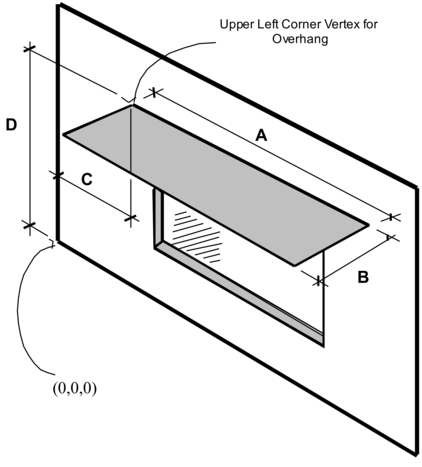
\includegraphics[width=0.9\textwidth, height=0.9\textheight, keepaspectratio=true]{media/image059.png}
\caption{Illustration for Attached Shading Surface \protect \label{fig:illustration-for-attached-shading-surface}}
\end{figure}

Proper specification for this overhang (facing up) is:

4,(C,0,D),(C,-B,D),(C+A,-B,D),(C+A,0,D); () used to illustrate each vertex.

\begin{callout}
Note that for horizontal surfaces, any corner may be chosen as the starting corner. The order of vertices determines whether the surface is facing up or down. Shading surfaces are mirrored automatically unless the user specifies ``DoNotMirrorDetachedShading'', so each shading surface need only be described once.
\end{callout}

Thus, another shading surface will be created (facing down):

4,(C+A,-B,D),(C+A,0,D),(C,0,D),(C,-B,D);

IDF example of attached shading surfaces (overhang, fin):

\begin{lstlisting}
Shading:Zone:Detailed,
  Zn001:Wall001:Shade001,       !- Surface Name
  Zn001:Wall001,                !- Base Surface Name
  ShadingTransmittance:0001,    !- Shadowing Transmittance Schedule
  4,                            !-RectangularOverhang
  1.524000 , -0.3050000    , 2.865000,
  1.524000 ,  0.0000000E+00, 2.865000,
  4.572000 ,  0.0000000E+00, 2.865000,
  4.572000 , -0.3050000    , 2.865000;

Shading:Zone:Detailed,
  Zn003:Wall001:Shade001,       !- Surface Name
  Zn003:Wall001,                !- Base Surface Name
  ShadingTransmittance:0001,    !- Shadowing Transmittance Schedule
  4,                            !-RectangularLeftFin
  57.97000 ,   8.450000    ,10.00000      ,
  57.97000 ,   8.450000    , 0.0000000E+00,
  57.97000 ,   6.450000    , 0.0000000E+00,
  57.97000 ,   6.450000    ,10.00000      ;

Shading:Zone:Detailed,
  Zn003:Wall001:Shade002,       !- Surface Name
  Zn003:Wall001,                !- Base Surface Name
  ShadingTransmittance:0003,    !- Shadowing Transmittance Schedule
  4,                            !-RectangularRightFin
  77.97000 ,   6.450000    ,10.00000      ,
  77.97000 ,   6.450000    , 0.0000000E+00,
  77.97000 ,   8.450000    , 0.0000000E+00,
  77.97000 ,   8.450000    ,10.00000      ;
\end{lstlisting}

\subsection{ShadingProperty:Reflectance}\label{shadingpropertyreflectance}

Specifies the reflectance properties of a shading surface when the solar reflection calculation has requested, i.e., when if ``WithReflections'' option is chosen in the Building object (ref: Building - Field: Solar Distribution). It is assumed that shading surfaces are divided into an unglazed, diffusely reflecting portion and a glazed, specularly-reflecting portion, either of which may be zero. The reflectance properties are assumed to be the same on both sides of the shading surface.

Note that a shadowing transmittance schedule (ref: Shading Surfaces, Field: Transmittance Schedule Name) can be used with a reflective shading surface. However, EnergyPlus assumes that the reflectance properties of the shading surface are constant even if the transmittance varies.

If no ShadingProperty:Reflectance objects are entered, the default values shown here will be used for shading surfaces. Other surfaces have their reflectance properties defined by the materials in the outer layers of the constructions.

\subsubsection{Inputs}\label{inputs-31-002}

\paragraph{Field: Shading Surface Name}\label{field-shading-surface-name}

The name of the Shading:Site, Shading:Building, Shading:Site:Detailed, Shading:Building:Detailed, Shading:Overhang, Shading:Overhang:Projection, Shading:Fin, Shading:Fin:Projection or Shading:Zone:Detailed object to which the following fields apply.

If this ShadingProperty:Reflectance object is not defined for a shading surface the default values listed in each of the following fields will be used in the solar reflection calculation.

\paragraph{Field: Diffuse Solar Reflectance of Unglazed Part of Shading Surface}\label{field-diffuse-solar-reflectance-of-unglazed-part-of-shading-surface}

The diffuse solar reflectance of the unglazed part of the shading surface (default = 0.2). This reflectance is assumed to be the same for beam-to-diffuse and diffuse-to-diffuse reflection. Beam-to-diffuse reflection is assumed to be independent of angle of incidence of beam radiation. Diffuse-to-diffuse reflection is assumed to be independent of angular distribution of the incident of diffuse radiation. The outgoing diffuse radiation is assumed to be isotropic (hemispherically uniform).

The sum of this reflectance and the shading surface transmittance should be less than or equal to 1.0.

\paragraph{Field: Diffuse Visible Reflectance of Unglazed Part of Shading Surface}\label{field-diffuse-visible-reflectance-of-unglazed-part-of-shading-surface}

The diffuse visible reflectance of the unglazed part of the shading surface (default = 0.2). This reflectance is assumed to be the same for beam-to-diffuse and diffuse-to-diffuse reflection. Beam-to-diffuse reflection is assumed to be independent of angle of incidence of beam radiation. Diffuse-to-diffuse reflection is assumed to be independent of angular distribution of the incident of diffuse radiation. The outgoing diffuse radiation is assumed to be isotropic (hemispherically uniform).

This value if used only for the daylighting calculation (ref: Daylighting:Controls). The sum of this reflectance and the shading surface transmittance should be less than or equal to 1.0.

\paragraph{Field: Fraction of Shading Surface That Is Glazed}\label{field-fraction-of-shading-surface-that-is-glazed}

The fraction of the area of the shading surface that consists of windows (default = 0.0). It is assumed that the windows are evenly distributed over the surface and have the same glazing construction (see following ``Name of Glazing Construction''). This might be the case, for example, for reflection from the façade of a neighboring, highly-glazed building. For the reflection calculation the possible presence of shades, screens or blinds on the windows of the shading surface is ignored. Beam-to-beam (specular) reflection is assumed to occur only from the glazed portion of the shading surface. This reflection depends on angle of incidence as determined by the program from the glazing construction. Beam-to-diffuse reflection from the glazed portion is assumed to be zero. The diffuse-to-diffuse reflectance of the glazed portion is determined by the program from the glazing construction.

\paragraph{Field: Glazing Construction Name}\label{field-glazing-construction-name}

The name of the construction of the windows on the shading surface. Required if Fraction of Shading Surface That Is Glazed is greater than 0.0.

IDF example of Shading Surface Reflectance for shading surface with specular reflection

\begin{lstlisting}

Shading:Site:Detailed,
  Adjacent Glazed Facade,  !- User Supplied Surface Name
  ,   !- Shadowing Transmittance Schedule
  4,  !- Number of Surface Vertex Groups -- Number of (X,Y,Z) groups
  0,-24,30, !- Vertex 1 X,Y,Z coordinates
  0,-24,0,  !- Vertex 2 X,Y,Z coordinates
  0,0,0,    !- Vertex 3 X,Y,Z coordinates
  0,0,30;   !-Vertex 3 X,Y,Z coordinates


  ShadingProperty:Reflectance,
  Adjacent Glazed Facade, !- Name of Surface:Shading Object
  0.3,  !- Diffuse Solar Reflectance of Unglazed Part of Shading Surface
  0.3,  !- Diffuse Visible Reflectance of Unglazed Part of Shading Surface
  0.7,  !- Fraction of Shading Surface That Is Glazed
  GlassCon-1; !- Name of Glazing Construction
\end{lstlisting}

IDF example of Shading Surface Reflectance for shading surface without specular reflection

\begin{lstlisting}

Shading:Site:Detailed,
  Adjacent Blank Facade,  !- User Supplied Surface Name
  ,   !- Shadowing Transmittance Schedule
  4,  !- Number of Surface Vertex Groups -- Number of (X,Y,Z) groups
  0,-24,30,
  0,-24,0,
  0,0,0,
  0,0,30;


  ShadingProperty:Reflectance,
  Adjacent Blank Facade, !- Name of Surface:Shading Object
  0.4,  !- Diffuse Solar Reflectance of Unglazed Part of Shading Surface
  0.4,  !- Diffuse Visible Reflectance of Unglazed Part of Shading Surface
  0.0,  !- Fraction of Shading Surface That Is Glazed
  ;     !- Name of glazing construction
\end{lstlisting}

\subsection{WindowShadingControl}\label{windowpropertyshadingcontrol}

Window shading with coverings like drapes, blinds, screens or pull-down shades can be used to reduce the amount of solar radiation entering the window or reduce daylighting glare. It can also be used to reduce heat loss through the window (movable insulation). Leaving the window covering open in the winter can maximize solar heat gain and thereby reduce heating loads.

With WindowShadingControl you specify the type and location of the shading device, what variable or combination of variables controls deployment of the shading device, and what the control setpoint is. If the shading device is a blind, you also specify how the slat angle is controlled. Each WindowShadingControl object is associated with a zone and has a list of one or more windows and glass doors to which the shading control is applied (ref: FenestrationSurface:Detailed with Type = Window or GlassDoor, Window, and GlazedDoor).

NOTE: WindowShadingControl does not work with complex fenestration systems. Controlled complex fenestration systems can be made only with Energy Management Systems objects. Refrencing a FenestrationSurface:Detailed in a WindowShadingControl while using complex fenestration systems will be ignored by program.

As shown in Figure~\ref{fig:allowed-locations-of-a-window-shading-device.}, a shading device can be inside the window (Shading Type = InteriorShade or InteriorBlind), outside the window (Shading Type = ExteriorShade or ExteriorBlind), or between panes of glass (Shading Type = BetweenGlassShade or BetweenGlassBlind). The exception is window screens which can only be outside the window (Shading Type = ExteriorScreen).

\begin{figure}[hbtp] % fig 34
\centering
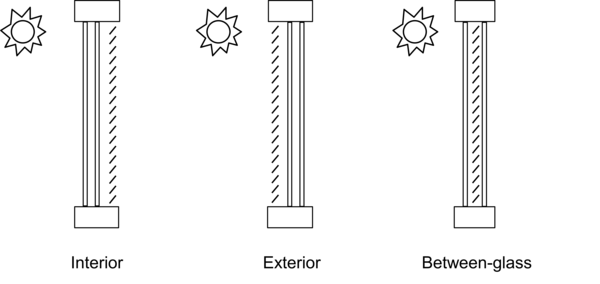
\includegraphics[width=0.9\textwidth, height=0.9\textheight, keepaspectratio=true]{media/image060.png}
\caption{Allowed locations of a window shading device. \protect \label{fig:allowed-locations-of-a-window-shading-device.}}
\end{figure}

When a shading device is present it is either retracted or activated. When it is retracted it covers none of the window. When it is activated it covers the entire glazed part of the window (but not the frame). Whether the shading device is retracted or activated in a particular timestep depends on the control mechanism: see ``Shading Control Type,'' below. To model a case in which the shading device, when activated, covers only \textbf{part} of the window you will have to divide the window into two separate windows, one with the shading device and one without the shading device.

A shading device can also be of a kind in which the optical properties of the glazing switch from one set of values to another in order to increase or decrease solar or visible transmittance (Shading Type = SwitchableGlazing).

There are two ways of specifying the actual shading device:

\begin{itemize}
  \item
\textbf{Specify ``Name of Construction with Shading''}

This is the name of a window Construction that has the shading device as one of its layers. The thermal and solar-optical properties of the shading device are given by the shading material referenced in that Construction (ref: Construction, WindowMaterial:Shade, WindowMaterial:Screen and WindowMaterial:Blind). To use this method you have to define two Constructions for the window, one without the shading device and one with it. See Example 1, below.

The Construction without the shading device is referenced in the FenestrationSurface:Detailed input for the window (see IDF example, below). The Construction with the shading device is referenced by the window's WindowShadingControl.

For Shading Type = InteriorShade, InteriorBlind, ExteriorShade, ExteriorScreen and ExteriorBlind these two Constructions must be identical expect for the presence of the shading layer in the shaded Construction, otherwise you will get an error message. You will also get an error message if the Construction referenced by the window has a shading layer.

  \item
\textbf{Specify the ``Material Name of the Shading Device''}

This is the name of a WindowMaterial:Shade, WindowMaterial:Screen or WindowMaterial:Blind. This method can be used with Shading Type = InteriorShade, InteriorBlind, ExteriorShade and ExteriorBlind. It cannot be used with Shading Type = BetweenGlassShade, BetweenGlassBlind, or SwitchableGlazing. If Shading Type = InteriorShade or ExteriorShade, then you specify the name of a WindowMaterial:Shade. If Shading Type = InteriorBlind or ExteriorBlind, then you specify the name of a WindowMaterial:Blind. If Shading Type = ExteriorScreen, then you specify the name of a WindowMaterial:Screen. See Example 2, below. This method is simpler to use since you don't have to specify two Constructions that differ only by the shading layer.

When this method is used, the program will automatically create a shaded window construction by adding a shading layer to the outside or inside of the construction corresponding to the windows referenced by the WindowShadingControl. The name, created by the program, of this shaded construction is composed as follows: if the name of the window construction is CCC and the material name of the shading device is DDD, then the shaded construction name is CCC:DDD:INT for an interior shading device and CCC:DDD:EXT for an exterior shading device.

This method is the required if you want to add a shading device to a construction brought in from a WINDOW Data File (ref:Construction:WindowDataFile).

Note that if both ``Name of Construction with Shading'' and ``Material Name of Shading Device'' are specified, the former takes precedence.
\end{itemize}

Most Shading Control Types allow you to specify a schedule that determines when the control is active. One example is a control that is active seasonally. For example, to deploy shading only in the summer when the incident solar is high enough, use Shading Control Type = OnIfHighSolarOnWindow with a schedule that is 1 during the summer months and 0 otherwise and specify Shading Control Is Scheduled = YES.

In addition, most Shading Control Types also allow you to specify that glare control is active in addition to the specified Control Type. For example, you might want to deploy shading when the solar incident on a window is too high OR the glare from the window is too high. This type of joint control requires that the window be in a daylit zone, that the maximum allowed glare be specified in the Daylighting object for the zone, and that Glare Control Is Active = YES in WindowShadingControl.

If Shading Type = InteriorBlind, ExteriorBlind or BetweenGlassBlind you can use WindowShadingControl to specify how the slat angle of the blind is controlled when the blind is in place.

A special type of WindowShadingControl is SwitchableGlazing. An example is electrochromic glazing in which the transmittance and reflectance of the glass is controlled electronically. For example, you could have electrochromic glazing switch from clear (high transmittance) to dark (low transmittance) to control solar gain. If you choose the Shading Type = SwitchableGlazing option for WindowShadingControl, the unswitched (clear) state is specified by the Construction referenced by the window and the switched (dark) state is specified by the Construction referenced by WindowShadingControl for that window. For example, if you specify Shading Type = SwitchableGlazing and Shading Control Type = OnIfHighSolarOnWindow, then the glazing will switch to the dark state whenever the solar radiation striking the window exceeds the Setpoint value.

For Shading Type = SwitchableGlazing the state of the window is either clear (unswitched) or dark (fully switched) for all Shading Control Types except MeetDaylightIlluminanceSetpoint. In this case, the transmittance of the glazing is adjusted to just meet the daylight illuminance set point at the first daylighting reference point (see Daylighting). This type of control assures that there is just enough solar gain to meet the daylighting requirements in a zone, and no more, thus reducing the cooling load.

To specify the order of when shades are deployed, the two different approaches can be used:

- If shades for each window are independently controlled, than a single WindowShadingControl object should be used and the Multiple Surface Control Type field should be set to Sequential. The windows should be specified in the Fenestration Surface N Name fields in the order that they should be deployed. The Shading Control Sequence Number field is not used being used since only one WindowShadingControl is used so it can be set to any value or left blank.

- If shades for a group of windows are deployed together and shades for another group of windows are deployed after that, than multiple WindowShadingControl objects should be used. Each WindowShadingControl should have Multiple Surface Control Type field should be set to Group and the names of each window in the group should be specified in the Fenestration Surface N Name fields. The Shading Control Sequence Number in the  WindowShadingControl object that controls the first group of shades should be set to 1. The Shading Control Sequence Number in the  WindowShadingControl object that controls the second group of shades should be set to 2. Any number of additional groups of shades can be added and Shading Control Sequence Number can be incremented by one for each group.

It is possible to mix these two approaches. For example, if first a group of shades is controlled together followed by a sequence of individual windows than these approaches can be combined with the Multiple Surface Control Type field should be set to Sequential in the second WindowShadingControl object.

\subsubsection{Inputs}\label{inputs-32-001}

\paragraph{Field: Name}\label{field-name-29-001}

Name of the window shading control.

\paragraph{Field: Zone Name}\label{field-zone-name-29-001}

Name of the zone where this shading control is used.

\paragraph{Field: Shading Control Sequence Number}\label{shading-control-sequence-number}

If multiple WindowShadingControl objects are used in the same zone, then the order that they deploy the window shades can be set with this field. The first WindowShadingControl should be 1 and subsequent WindowShadingControl should 2, 3, etc. This is usually used when the Multiple Surface Control Type field is set to Group to control groups of windows in a certain order.

\paragraph{Field: Shading Type}\label{field-shading-type}

The type of shading device. The choices are:

\emph{InteriorShade}: A diffusing shade is on the inside of the window. (In the shaded Construction the shading layer must be a WindowMaterial:Shade.)

\emph{ExteriorShade}: A diffusing shade is on the outside of the window. (In the shaded Construction the shading layer must be a WindowMaterial:Shade.)

\emph{BetweenGlassShade}: A diffusing shade is between two glass layers. (In the shaded Construction the shading layer must be a WindowMaterial:Shade.) This shading type is allowed only for double- and triple-glazing. For triple-glazing the shade must be between the two inner glass layers.

\emph{ExteriorScreen}: An insect screen is on the outside of the window. (In the shaded Construction the shading layer must be a WindowMaterial:Screen.)

\emph{InteriorBlind}: A slat-type shading device, such as a Venetian blind, is on the inside of the window. (In the shaded Construction the shading layer must be a WindowMaterial:Blind.)

\emph{ExteriorBlind}: A slat-type shading device is on the outside of the window. (In the shaded Construction the shading layer must be a WindowMaterial:Blind.)

\emph{BetweenGlassBlind}: A slat-type shading device is between two glass layers. (In the shaded Construction the shading layer must be a WindowMaterial:Blind.) This shading type is allowed only for double- and triple-glazing. For triple-glazing the blind must be between the two inner glass layers.

\emph{SwitchableGlazing}: Shading is achieved by changing the characteristics of the window glass, such as by darkening it.

\paragraph{Field: Construction with Shading Name}\label{field-construction-with-shading-name}

Name of the window Construction that has the shading in place. The properties of the shading device are given by the shading material referenced in that Construction (ref: Construction, WindowMaterial:Shade, WindowMaterial:Screen and WindowMaterial:Blind). For Shading Type = SwitchableGlazing, this is the name of the Construction that corresponds to the window in its fully-switched (darkest) state.

Specifying ``Name of Construction with Shading'' is required if Shading Type = BetweenGlassShade, BetweenGlassBlind, or SwitchableGlazing. For other Shading Types, you may alternatively specify ``Material Name of Shading Device'' (see below).

\paragraph{Field: Shading Control Type}\label{field-shading-control-type}

Specifies how the shading device is controlled, i.e., it determines whether the shading device is ``on'' or ``off.'' For blinds, screens and shades, when the device is ``on'' it is assumed to cover all of the window except its frame; when the device is ``off'' it is assumed to cover none of the window (whether ``on'' or ``off'' the shading device is assumed to cover none of the wall that the window is on).

For switchable glazing, ``on'' means that the glazing is in the fully-switched state and ``off'' means that it is in the unswitched state; for example, for electrochromic glazing, ``on'' means the glazing is in its darkest state and ``off'' means it is in its lightest state.

The choices for Shading Control Type are the following. If SetPoint is applicable its units are shown in parentheses.

\emph{AlwaysOn}: Shading is always on.

\emph{AlwaysOff}: Shading is always off.

The following six control types are used primarily to reduce zone cooling load due to window solar gain.

\emph{OnIfScheduleAllows}: Shading is on if schedule value is non-zero. Requires that Schedule Name be specified and Shading Control Is Scheduled = Yes.

Note: For exterior window screens \emph{AlwaysOn, AlwaysOff, and OnIfScheduleAllows} are the only valid shading control types.

\emph{OnIfHighSolarOnWindow}: Shading is on if beam plus diffuse solar radiation incident on the window exceeds SetPoint (W/m\(^{2}\)) and schedule, if specified, allows shading.

\emph{OnIfHighHorizontalSolar}: Shading is on if total (beam plus diffuse) horizontal solar irradiance exceeds SetPoint (W/m\(^{2}\)) and schedule, if specified, allows shading.

\emph{OnIfHighOutdoorAirTemperature}: Shading is on if outside air temperature exceeds SetPoint (C) and schedule, if specified, allows shading.

\emph{OnIfHighZoneAirTemperature}: Shading is on if zone air temperature in the previous timestep exceeds SetPoint (C) and schedule, if specified, allows shading.

\emph{OnIfHighZoneCooling}: Shading is on if zone cooling rate in the previous timestep exceeds SetPoint (W) and schedule, if specified, allows shading.

\emph{OnIfHighGlare}: Shading is on if the total daylight glare index at the zone's first daylighting reference point from all of the exterior windows in the zone exceeds the maximum glare index specified in the daylighting input for zone (ref: Group -- Daylighting). Applicable only to windows in zones with daylighting.

Note: Unlike other Shading Control Types, glare control is active whether or not a schedule is specified.

\emph{MeetDaylightIlluminanceSetpoint}: Used only with ShadingType = SwitchableGlazing in zones with daylighting controls. In this case the transmittance of the glazing is adjusted to just meet the daylight illuminance set point at the first daylighting reference point. Note that the daylight illuminance set point is specified in the Daylighting:Controls object for the Zone; it is not specified as a WindowShadingControl SetPoint. When the glare control is active, if meeting the daylight illuminance set point at the first daylighting reference point results in higher discomfort glare index (DGI) than the specified zone's maximum allowable DGI for either of the daylight reference points, the glazing will be further dimmed until the DGI equals the specified maximum allowable value.

The following three control types can be used to reduce zone heating load during the winter by reducing window conductive heat loss at night and leaving the window unshaded during the day to maximize solar gain. They are applicable to any Shading Type except ExteriorScreen but are most appropriate for interior or exterior shades with high insulating value (``movable insulation''). ``Night'' means the sun is down and ``day'' means the sun is up.

\emph{OnNightIfLowOutdoorTempAndOffDay}: Shading is on at night if the outside air temperature is less than SetPoint (C) and schedule, if specified, allows shading. Shading is off during the day.

\emph{OnNightIfLowInsideTempAndOffDay}: Shading is on at night if the zone air temperature in the previous timestep is less than SetPoint (C) and schedule, if specified, allows shading. Shading is off during the day.

\emph{OnNightIfHeatingAndOffDay}: Shading is on at night if the zone heating rate in the previous timestep exceeds SetPoint (W) and schedule, if specified, allows shading. Shading is off during the day.

The following two control types can be used to reduce zone heating and cooling load. They are applicable to any Shading Type except ExteriorScreen but are most appropriate for translucent interior or exterior shades with high insulating value (``translucent movable insulation'').

\emph{OnNightIfLowOutdoorTempAndOnDayIfCooling}: Shading is on at night if the outside air temperature is less than SetPoint (C). Shading is on during the day if the zone cooling rate in the previous timestep is non-zero. Night and day shading is subject to schedule, if specified.

\emph{OnNightIfHeatingAndOnDayIfCooling}: Shading is on at night if the zone heating rate in the previous timestep exceeds SetPoint (W). Shading is on during the day if the zone cooling rate in the previous timestep is non-zero. Night and day shading is subject to schedule, if specified.

The following control types can be used to reduce zone cooling load. They are applicable to any Shading Type except ExteriorScreen but are most appropriate for interior or exterior blinds, interior or exterior shades with low insulating value, or switchable glazing.

\emph{OffNightAndOnDayIfCoolingAndHighSolarOnWindow}: Shading is off at night. Shading is on during the day if the solar radiation incident on the window exceeds SetPoint (W/m\(^{2}\)) and if the zone cooling rate in the previous timestep is non-zero. Daytime shading is subject to schedule, if specified.

\emph{OnNightAndOnDayIfCoolingAndHighSolarOnWindow}: Shading is on at night. Shading is on during the day if the solar radiation incident on the window exceeds SetPoint (W/m\(^{2}\)) and if the zone cooling rate in the previous timestep is non-zero. Day and night shading is subject to schedule, if specified. (This Shading Control Type is the same as the previous one, except the shading is on at night rather than off.)

\emph{OnIfHighOutdoorAirTempAndHighSolarOnWindow:} Shading is on if the outside air temperature exceeds the Setpoint (C) and if if the solar radiation incident on the window exceeds SetPoint 2 (W/m\(^{2}\)).

\emph{OnIfHighOutdoorAirTempAndHighHorizontalSolar:} Shading is on if the outside air temperature exceeds the Setpoint (C) and if if the horizontal solar radiation exceeds SetPoint 2 (W/m\(^{2}\)).

\paragraph{Field: Schedule Name}\label{field-schedule-name-007}

Required if Shading Control Is Scheduled = Yes. If schedule value \textgreater{} 0 , shading control is active, i.e., shading can be on only if the shading control test passes. If schedule value = 0, shading is off whether or not the control test passes. If Schedule Name is not specified, shading control is assumed to be active at all times.

\paragraph{Field: Setpoint}\label{field-setpoint}

The setpoint for activating window shading. The units depend on the type of trigger:

\begin{itemize}
\item
  W/m\(^{2}\) for solar-based controls
\item
  W for cooling- or heating-based controls
\item
  Degrees C for temperature-based controls
\end{itemize}

SetPoint is unused for Shading Control Type = OnIfScheduleAllows, OnIfHighGlare and DaylightIlluminance.

\paragraph{Field: Shading Control Is Scheduled}\label{field-shading-control-is-scheduled}

Accepts values YES and NO. The default is NO. Not applicable for Shading Control Type = OnIfHighGlare and should be blank in that case.

If YES, Schedule Name is required and that schedule determines whether the shading control specified by Shading Control Type is active or inactive (see Schedule Name, above).

If NO, Schedule Name is not applicable (should be blank) and the shading control is unscheduled.

Shading Control Is Scheduled = YES is required if Shading Control Type = OnIfScheduleAllows.

\paragraph{Field: Glare Control Is Active}\label{field-glare-control-is-active}

Accepts values YES and NO. The default is NO.

If YES and the window is in a daylit zone, shading is on if the zone's discomfort glare index exceeds the maximum discomfort glare index specified in the Daylighting object referenced by the zone. For switchable windows with \emph{MeetDaylightIlluminanceSetpoint} shading control, if Glare Control is active, the windows are always continuously dimmed as necessary to meet the zone's maximum allowable DGI while providing appropriate amount of daylight for the zone.

The glare test is OR'ed with the test specified by Shading Control Type. For example, if Glare Control Is Active = YES and Shading Control Type = OnIfHighZoneAirTemp, then shading is on if glare is too high OR if the zone air temperature is too high.

Glare Control Is Active = YES is required if Shading Control Type = OnIfHighGlare.

\paragraph{Field: Shading Device Material Name}\label{field-shading-device-material-name}

The name of a WindowMaterial:Shade, WindowMaterial:Screen or WindowMaterial:Blind. Required if ``Name of Construction with Shading'' is not specified. Not applicable if Shading Type = BetweenGlassShade, BetweenGlassBlind or SwitchableGlazing and should be blank in this case. If both ``Name of Construction with Shading'' and ``Material Name of Shading Device'' are entered the former takes precedence.

\paragraph{Field: Type of Slat Angle Control for Blinds}\label{field-type-of-slat-angle-control-for-blinds}

Applies only to Shading Type = InteriorBlind, ExteriorBlind or BetweenGlassBlind. Specifies how the slat angle is controlled. The choices are FixedSlatAngle, ScheduledSlatAngle and BlockBeamSolar.

If FixedSlatAngle (the default), the angle of the slat is fixed at the value input for the WindowMaterial:Blind that is contained in the construction specified by Name of Construction with Shading or is specified by Material Name of Shading Device.

If ScheduledSlatAngle, the slat angle varies according to the schedule specified by Slat Angle Schedule Name, below.

If BlockBeamSolar, the slat angle is set each timestep to just block beam solar radiation. If there is no beam solar on the window the slat angle is set to the value input for the WindowMaterial:Blind that is contained in the construction specified by Name of Construction with Shading or is specified by Material Name of Shading Device. The BlockBeamSolar option prevents beam solar from entering the window and causing possible unwanted glare if the beam falls on work surfaces while at the same time allowing near-optimal indirect radiation for daylighting.

\paragraph{Field: Slat Angle Schedule Name}\label{field-slat-angle-schedule-name}

This is the name of a schedule of slat angles that is used when Type of Slat Angle Control for Blinds = ScheduledSlatAngle. You should be sure that the schedule values fall within the range given by the Minimum Slat Angle and Maximum Slat Angle values entered in the corresponding WindowMaterial:Blind. If not, the program will force them into this range.

\paragraph{Field: Setpoint 2}\label{field-setpoint-2}

Used only as the second setpoint for the following two-setpoint control types: OnIfHighOutdoorAirTempAndHighSolarOnWindow, OnIfHighOutdoorAirTempAndHighHorizontalSolar, OnIfHighZoneAirTempAndHighSolarOnWindow, and OnIfHighZoneAirTempAndHighHorizontalSolar

\paragraph{Field: Daylighting Controls Object Name}\label{field-daylighting-controls-object-name}

Name of the Daylighting:Controls object that provides the glare and illuminance control to the zone.

\paragraph{Field: Multiple Surface Control Type}\label{field-multiple-surface-control-type}

The field can have one of two options:

\emph{Sequential}: The following list of fenestration surfaces are controlled individually in the order specified.

\emph{Group}: The entire list of fenestration surfaces is controlled simultaneously, and if glare control is needed, the entire group of window shades are deployed together a the same time.

\paragraph{Field: Fenestration Surface <n> Name}\label{field-fenestration-surface1-name}

The name of a FenestrationSurface:Detailed, Window, or GlazedDoor object controlled by this WindowShadingControl. This field can be repeated to apply the same shading control to more than one fenestration surface. When Multiple Surface Control Type is set to Sequential, the order of the Fenestration Surface Names is the order that the shades will be deployed. The object is extensible so that additional fields of fenestration surface names can be added to the object. All of the fenestration surfaces must be either in the zone specified in the Zone Name field or in an adjacent zone connected by an interior window.

An IDF example: window with interior roll shade that is deployed when solar incident on the window exceeds 50 W/m\(^{2}\).

\begin{lstlisting}
! Example 1: Interior movable shade specified by giving name of shaded construction
! in WindowShadingControl

WindowMaterial:Glazing, GLASS - CLEAR SHEET 1 / 8 IN,  !- Material Name
       SpectralAverage,! Optical data type {SpectralAverage or Spectral}
       ,               ! Name of spectral data set when Optical Data Type = Spectral
       0.003        ,  !- Thickness {m}
       0.837        ,  !- Solar Transmittance at Normal Incidence
       0.075        ,  !- Solar Reflectance at Normal Incidence: Front Side
       0.075        ,  !- Solar Reflectance at Normal Incidence: Back Side
       0.898        ,  !- Visible Transmittance at Normal Incidence
       0.081        ,  !- Visible Reflectance at Normal Incidence: Front Side
       0.081        ,  !- Visible Reflectance at Normal Incidence: Back Side
       0.0          ,  !- IR Transmittance
       0.8400000    ,  !- IR Emissivity: Front Side
       0.8400000    ,  !- IR Emissivity: Back Side
       0.9000000    ;  !- Conductivity {W/m-K}

WindowMaterial:Shade, ROLL SHADE,  !- Material Name
       0.3          ,   !- Solar Transmittance at normal incidence
       0.5000000    ,   !- Solar Reflectance (same for front and back side)
       0.3          ,   !- Visible Transmittance at normal incidence
       0.5000000    ,   !- Visible reflectance (same for front and back side)
       0.9000000    ,   !- IR Emissivity (same for front and back side)
       0.05         ,   !- IR Transmittance
       0.003        ,   !- Thickness
       0.1          ,   !- Conductivity {W/m-K}
       0.0          ,   !- Top Opening Multiplier
       0.0          ,   !- Bottom Opening Multiplier
       0.5          ,   !- Left-Side Opening Multiplier
       0.5          ,   !- Right-Side Opening Multiplier
       0.0          ;   !- Air-Flow Permeability

Construction, SINGLE PANE WITH NO SHADE,  ! Name of construction without shade
       GLASS - CLEAR SHEET 1 / 8 IN;  !- First material layer

Construction, SINGLE PANE WITH INT SHADE, ! Name of construction with shade
       GLASS - CLEAR SHEET 1 / 8 IN,  !- First material layer
       ROLL SHADE                  ;  !- Second material layer

WindowShadingControl, 
       CONTROL ON INCIDENT SOLAR,    !- Name
       West Zone,                    !- Zone Name
       1,                            !- Shading Control Sequence Number
       InteriorShade,                !- Shading Type
       SINGLE PANE WITH INT SHADE,   !- Name of construction with shading device
       OnIfHighSolarOnWindow,        !- Shading Control Type
       ,                             !- Schedule name
       50.0,                         !- Setpoint {W/m2}
       NO,                           !- Shading Control Is Scheduled
       NO,                           !- Glare Control Is Active
       ,                             !- Material Name of Shading Device
       ,                             !- Type of Slat Angle Control for Blinds
       ,                             !- Slat Angle Schedule Name
       ,                             !- Setpoint 2 {W/m2 or deg C}
       West Zone_DaylCtrl,           !- Daylighting Control Object Name
       Sequential,                   !- Multiple Surface Control Type
       Zn001:Wall001:Win001;         !- Fenestration Surface 1 Name

FenestrationSurface:Detailed, 
       Zn001:Wall001:Win001,         !- SubSurface Name
       Window                   ,    !- Class
       SINGLE PANE WITH NO SHADE,    !- Name of construction without shading device
       Zn001:Wall001            ,    !- Base Surface Name
       ,                             !- Target
       0.5000000                ,    !- VF to Ground
       ,                             !- Frame/Divider name
       1.0                      ,    !- Multiplier
       4                        ,    !- Number of vertices (assumed rectangular)
       0.548 ,  0.0 ,   2.5     ,    !- x,y,z of vertices {m}
       0.548 ,  0.0 ,   0.5     ,
       5.548 ,  0.0 ,   0.5     ,
       5.548 ,  0.0 ,   2.5     ;
\end{lstlisting}

\begin{lstlisting}
! Example 2: Interior movable shade specified by giving name of shading device in WindowShadingControl

WindowMaterial:Glazing, GLASS - CLEAR SHEET 1 / 8 IN,  !- Material Name
       SpectralAverage,! Optical data type {SpectralAverage or Spectral}
       ,               ! Name of spectral data set when Optical Data Type = Spectral
       0.003        ,  !- Thickness {m}
       0.837        ,  !- Solar Transmittance at Normal Incidence
       0.075        ,  !- Solar Reflectance at Normal Incidence: Front Side
       0.075        ,  !- Solar Reflectance at Normal Incidence: Back Side
       0.898        ,  !- Visible Transmittance at Normal Incidence
       0.081        ,  !- Visible Reflectance at Normal Incidence: Front Side
       0.081        ,  !- Visible Reflectance at Normal Incidence: Back Side
       0.0          ,  !- IR Transmittance
       0.8400000    ,  !- IR Emissivity: Front Side
       0.8400000    ,  !- IR Emissivity: Back Side
       0.9000000    ;  !- Conductivity {W/m-K}

WindowMaterial:Shade, ROLL SHADE,  !- Material Name
       0.3          ,   !- Solar Transmittance at normal incidence
       0.5000000    ,   !- Solar Reflectance (same for front and back side)
       0.3          ,   !- Visible Transmittance at normal incidence
       0.5000000    ,   !- Visible reflectance (same for front and back side)
       0.9000000    ,   !- IR Emissivity (same for front and back side)
       0.05         ,   !- IR Transmittance
       0.003        ,   !- Thickness
       0.1          ,   !- Conductivity {W/m-K}
       0.0          ,   !- Top Opening Multiplier
       0.0          ,   !- Bottom Opening Multiplier
       0.5          ,   !- Left-Side Opening Multiplier
       0.5          ,   !- Right-Side Opening Multiplier
       0.0          ;   !- Air-Flow Permeability

Construction, SINGLE PANE WITH NO SHADE,  ! Name of construction without shade
       GLASS - CLEAR SHEET 1 / 8 IN;  !- First material layer

WindowShadingControl, 
       CONTROL ON INCIDENT SOLAR,    !- Name
       West Zone,                    !- Zone Name
       1,                            !- Shading Control Sequence Number
       InteriorShade,                !- Shading Type
       ,                             !- Name of shaded construction
       OnIfHighSolarOnWindow,        !- Shading Control Type
       ,                             !- Schedule name
       50.0,                         !- Setpoint {W/m2}
       NO,                           !- Shading Control Is Scheduled
       NO,                           !- Glare Control Is Active
       ROLL SHADE,                   !- Material Name of Shading Device
       ,                             !- Type of Slat Angle Control for Blinds
       ,                             !- Slat Angle Schedule Name
       ,                             !- Setpoint 2 {W/m2 or deg C}
       West Zone_DaylCtrl,           !- Daylighting Control Object Name
       Sequential,                   !- Multiple Surface Control Type
       Zn001:Wall001:Win001;         !- Fenestration Surface 1 Name

FenestrationSurface:Detailed, 
       Zn001:Wall001:Win001,         !- SubSurface Name
       Window                   ,    !- Class
       SINGLE PANE WITH NO SHADE,    !- Name of construction without shade
       Zn001:Wall001            ,    !- Base Surface Name
       ,                             !- Target
       0.5000000                ,    !- VF to Ground
       ,                             !- Frame/Divider name
       1.0                      ,    !- Multiplier
       4                        ,    !- Number of vertices (assumed rectangular)
       0.548 ,  0.0 ,   2.5     ,    !- x,y,z of vertices {m}
       0.548 ,  0.0 ,   0.5     ,
       5.548 ,  0.0 ,   0.5     ,
       5.548 ,  0.0 ,   2.5     ;
\end{lstlisting}

\subsection{WindowProperty:FrameAndDivider}\label{windowpropertyframeanddivider}

The WindowProperty:FrameAndDivider object is referenced by exterior windows that have

\begin{itemize}
\item
  a frame, and/or
\item
  a divider, and/or
\item
  reveal surfaces that reflect beam solar radiation.
\end{itemize}

A \textbf{\emph{frame}} surrounds the glazing in a window (see Figure~\ref{fig:a-window-with-a-frame-and-divider.} and Figure~\ref{fig:illustration-showing-frame-and-divider}). It is assumed that all frame characteristics---such as width, conductance and solar absorptance---are the same for the top, bottom and side elements of the frame. If the frame elements are not the same then you should enter area-weighted average values for the frame characteristics.

The window vertices that you specify in the FenestrationSurface:Detailed object are those of the glazed part of the window, not the frame. EnergyPlus automatically subtracts the area of the frame---determined from the glazing dimensions and the frame width---from the area of the wall containing the window.

A \textbf{\emph{divider}}, as shown in Figure~\ref{fig:a-window-with-a-frame-and-divider.}, Figure~\ref{fig:illustration-showing-frame-and-divider} and Figure~\ref{fig:illustration-showing-divider-types.}, divides the glazing up into separate lites. It is assumed that all divider elements have the same characteristics. If not, area-weighted average values should be used. EnergyPlus automatically subtracts the divider area from the glazed area of the window.

\textbf{\emph{Reveal surfaces}}, as shown in Figure~\ref{fig:a-vertical-section-through-a-window-with}, are associated with the setback of the glazing from the outside and/or inside surface of the parent wall. If the depth and solar absorptance of these surfaces are specified, the program will calculate the reflection of beam solar radiation from these surfaces. The program also calculates the shadowing (onto the window) of beam and diffuse solar radiation by outside reveal surfaces.

In EnergyPlus, a window can have any combination of frame, divider and reveal surfaces, or none of these.

The best source of frame and divider characteristics is the WINDOW program, which will calculate the values required by EnergyPlus for different frame and divider types. In particular, the THERM program within the WINDOW program will calculate the effective conductance of frames and dividers; this is the conductance taking 2-D heat transfer effects into account.

Note that a window's frame and divider characteristics, along with other window information, can be read in from the Window Data File (see ``Importing Windows from the WINDOW program'' and ``Construction:WindowDataFile object''). In this case the WindowProperty:FrameAndDivider referenced by the window is not applicable and should be blank unless you want to specify reveal surfaces for beam solar reflection.

\begin{figure}[hbtp] % fig 35
\centering
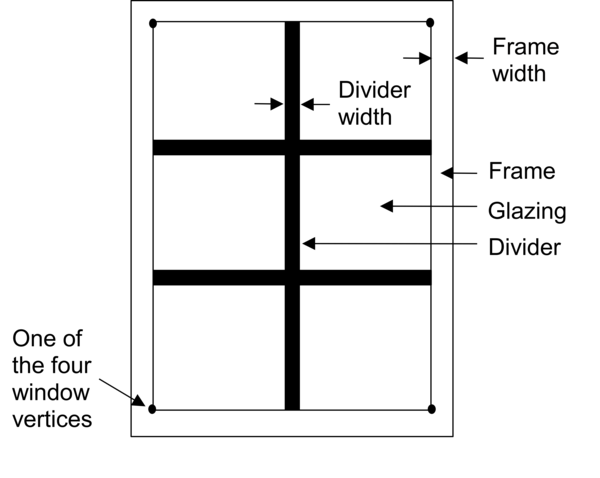
\includegraphics[width=0.9\textwidth, height=0.9\textheight, keepaspectratio=true]{media/image061.png}
\caption{A window with a frame and divider. \protect \label{fig:a-window-with-a-frame-and-divider.}}
\end{figure}

In the illustration above, the divider has two horizontal elements and one vertical element.

\subsubsection{Inputs}\label{inputs-33-001}

\paragraph{Field: Name}\label{field-name-30-001}

The name of the frame/divider object. It is referenced by WindowProperty:FrameAndDivider Name in FenestrationSurface:Detailed.

\textbf{\emph{Frame Fields}}

\paragraph{Field: Frame Width}\label{field-frame-width}

The width of the frame elements when projected onto the plane of the window. It is assumed that the top, bottom and side elements of the frame have the same width. If not, an average frame width should be entered such that the projected frame area calculated using the average value equals the sum of the areas of the frame elements.

\paragraph{Field: Frame Outside Projection}\label{field-frame-outside-projection}

The amount by which the frame projects outward from the outside surface of the window glazing. If the outer surface of the frame is flush with the glazing, Frame Outside Projection = 0.0. Used to calculate shadowing of frame onto glass, solar absorbed by frame, IR emitted and absorbed by frame, and convection from frame.

\paragraph{Field: Frame Inside Projection}\label{field-frame-inside-projection}

The amount by which the frame projects inward from the inside surface of the window glazing. If the inner surface of the frame is flush with the glazing, Frame Inside Projection = 0.0. Used to calculate solar absorbed by frame, IR emitted and absorbed by frame, and convection from frame.

\begin{figure}[hbtp] % fig 36
\centering
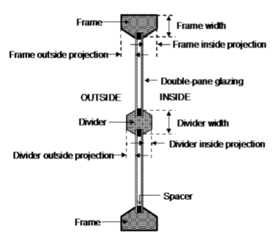
\includegraphics[width=0.9\textwidth, height=0.9\textheight, keepaspectratio=true]{media/image062.png}
\caption{Illustration showing frame and divider dimensioning. \protect \label{fig:illustration-showing-frame-and-divider}}
\end{figure}

\paragraph{Field: Frame Conductance}\label{field-frame-conductance}

The effective thermal conductance of the frame measured from inside to outside frame surface (no air films) and taking 2-D conduction effects into account. Obtained from the WINDOW program or other 2-D calculation.

\paragraph{Field: Ratio of Frame-Edge Glass Conductance to Center-Of-Glass Conductance}\label{field-ratio-of-frame-edge-glass-conductance-to-center-of-glass-conductance}

The glass conductance near the frame (excluding air films) divided by the glass conductance at the center of the glazing (excluding air films). Used only for multi-pane glazing constructions. This ratio is greater than 1.0 because of thermal bridging from the glazing across the frame and across the spacer that separates the glass panes. Values can be obtained from the WINDOW program the user-selected glazing construction and frame characteristics.

\paragraph{Field: Frame Solar Absorptance}\label{field-frame-solar-absorptance}

The solar absorptance of the frame. The value is assumed to be the same on the inside and outside of the frame and to be independent of angle of incidence of solar radiation. If solar reflectance (or reflectivity) data is available, then absorptance is equal to 1.0 minus reflectance (for opaque materials).

\paragraph{Field: Frame Visible Absorptance}\label{field-frame-visible-absorptance}

The visible absorptance of the frame. The value is assumed to be the same on the inside and outside of the frame and to be independent of angle of incidence of solar radiation. If visible reflectance (or reflectivity) data is available, then absorptance is equal to 1.0 minus reflectance (for opaque materials).

\paragraph{Field: Frame Thermal Hemispherical Emissivity}\label{field-frame-thermal-hemispherical-emissivity}

The thermal emissivity of the frame, assumed the same on the inside and outside.

\textbf{\emph{Divider Fields}}

\paragraph{Field: Divider Type}\label{field-divider-type}

The type of divider (see figure below). Divider Type = Suspended is applicable only to multi-pane glazing. It means that the divider is suspended between the panes. (If there are more than two glass layers, the divider is assumed to be placed between the two outermost layers.)

Divider Type = DividedLite means that the divider elements project out from the outside and inside surfaces of the glazing and divide the glazing into individual lites. For multi-pane glazing, this type of divider also has between-glass elements that separate the panes.

\begin{figure}[hbtp] % fig 37
\centering
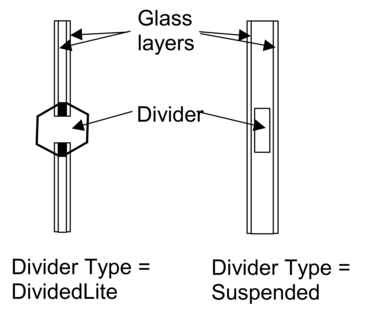
\includegraphics[width=0.9\textwidth, height=0.9\textheight, keepaspectratio=true]{media/image063.png}
\caption{Illustration showing divider types. \protect \label{fig:illustration-showing-divider-types.}}
\end{figure}

\paragraph{Field: Divider Width}\label{field-divider-width}

The width of the divider elements when projected onto the plane of the window. It is assumed that the horizontal and vertical divider elements have the same width. If not, an average divider width should be entered such that the projected divider area calculated using the average value equals the sum of the areas of the divider elements.

\paragraph{Field: Number of Horizontal Dividers}\label{field-number-of-horizontal-dividers}

The number of divider elements parallel to the top and bottom of the window.

\paragraph{Field: Number of Vertical Dividers}\label{field-number-of-vertical-dividers}

The number of divider elements parallel to the sides of the window.

\paragraph{Field: Divider Outside Projection}\label{field-divider-outside-projection}

The amount by which the divider projects out from the outside surface of the window glazing. For Divider Type = Suspended, Divider Projection = 0.0. Used to calculate shadowing of divider onto glass, solar absorbed by divider, IR emitted and absorbed by divider, and convection from divider.

\paragraph{Field: Divider Inside Projection}\label{field-divider-inside-projection}

The amount by which the divider projects inward from the inside surface of the window glazing. If the inner surface of the divider is flush with the glazing, Divider Inside Projection = 0.0. Used to calculate solar absorbed by divider, IR emitted and absorbed by divider, and convection from divider.

\paragraph{Field: Divider Conductance}\label{field-divider-conductance}

The effective thermal conductance of the divider measured from inside to outside divider surface (no air films) and taking 2-D conduction effects into account. Obtained from the WINDOW program or other 2-D calculation.

\paragraph{Field: Ratio of Divider-Edge Glass Conductance to Center-Of-Glass Conductance}\label{field-ratio-of-divider-edge-glass-conductance-to-center-of-glass-conductance}

The glass conductance near the divider (excluding air films) divided by the glass conductance at the center of the glazing (excluding air films). Used only for multi-pane glazing constructions. This ratio is greater than 1.0 because of thermal bridging from the glazing across the divider and across the spacer that separates the glass panes. Values can be obtained from the WINDOW program for the user-selected glazing construction and divider characteristics.

\paragraph{Field: Divider Solar Absorptance}\label{field-divider-solar-absorptance}

The solar absorptance of the divider. The value is assumed to be the same on the inside and outside of the divider and to be independent of angle of incidence of solar radiation. If solar reflectance (or reflectivity) data is available, then absorptance is equal to 1.0 minus reflectance (for opaque materials).

\paragraph{Field: Divider Visible Absorptance}\label{field-divider-visible-absorptance}

The visible absorptance of the divider. The value is assumed to be the same on the inside and outside of the divider and to be independent of angle of incidence of solar radiation. If visible reflectance (or reflectivity) data is available, then absorptance is equal to 1.0 minus reflectance (for opaque materials).

\paragraph{Field: Divider Thermal Hemispherical Emissivity}\label{field-divider-thermal-hemispherical-emissivity}

The thermal emissivity of the divider, assumed the same on the inside and outside.

\textbf{\emph{Reveal Surface Fields}}

The following fields specify the properties of the window reveal surfaces (reveals occur when the window is not in the same plane as the base surface). From this information and from the geometry of the window and the sun position, the program calculates beam solar radiation absorbed and reflected by the top, bottom, right and left sides of outside and inside window reveal surfaces. In doing this calculation, the shadowing on a reveal surface by other reveal surfaces is determined using the orientation of the reveal surfaces and the sun position.

It is assumed that:

\begin{itemize}
\item
  The window is an exterior window.
\item
  The reveal surfaces are perpendicular to the window plane.
\item
  If an exterior shade, screen or blind is in place it shades exterior and interior reveal surfaces so that in this case there is no beam solar on these surfaces.
\item
  If an interior shade or blind is in place it shades the interior reveal surfaces so that in this case there is no beam solar on these surfaces.
\item
  The possible shadowing on inside reveal surfaces by a window divider is ignored.
\item
  The outside reveal surfaces (top, bottom, left, right) have the same solar absorptance and depth. This depth is not input here but is automatically determined by the program---from window and wall vertices--as the distance between the plane of the outside face of the glazing and plane of the outside face of the parent wall.
\item
  The inside reveal surfaces are divided into two categories: (1) the bottom reveal surface, called here the ``inside sill;'' and (2) the other reveal surfaces (left, right and top).
\item
  The left, right and top inside reveal surfaces have the same depth and solar absorptance. The inside sill is allowed to have depth and solar absorptance values that are different from the corresponding values for the other inside reveal surfaces.
\item
  The inside sill depth is required to be greater than or equal to the depth of the other inside reveal surfaces. If the inside sill depth is greater than zero the depth of the other inside reveal surfaces is required to be greater than zero.
\item
  The reflection of beam solar radiation from all reveal surfaces is assumed to be isotropic diffuse; there is no specular component.
\item
  Half of the beam solar reflected from outside reveal surfaces is goes towards the window; the other half goes back to the exterior environment (i.e., reflection of this outward-going component from other outside reveal surfaces is not considered).
\item
  The half that goes towards the window is added to the other solar radiation incident on the window. Correspondingly, half of the beam solar reflected from inside reveal surfaces goes towards the window, with the other half going into the zone. The portion going towards the window that is not reflected is absorbed in the glazing or is transmitted back out into the exterior environment.
\item
  The beam solar that is absorbed by outside reveal surfaces is added to the solar absorbed by the outside surface of the window's parent wall; similarly, the beam solar absorbed by the inside reveal surfaces is added to the solar absorbed by the inside surface of the parent wall.
\end{itemize}

The net effect of beam solar reflected from outside reveal surfaces is to increase the heat gain to the zone, whereas the effect of beam solar reflected from inside reveal surfaces is to decrease the heat gain to the zone since part of this reflected solar is transmitted back out the window.

~If the window has a frame, the absorption of reflected beam solar by the inside and outside surfaces of the frame is considered. The shadowing of the frame onto interior reveal surfaces is also considered.

\paragraph{Field: Outside Reveal Solar Absorptance}\label{field-outside-reveal-solar-absorptance}

The solar absorptance of outside reveal surfaces.

\paragraph{Field: Inside Sill Depth}\label{field-inside-sill-depth}

The depth of the inside sill, measured from the inside surface of the glazing to the edge of the sill (see Figure~\ref{fig:a-vertical-section-through-a-window-with}).

\paragraph{Field: Inside Sill Solar Absorptance}\label{field-inside-sill-solar-absorptance}

The solar absorptance of the inside sill.

\textbf{\emph{Field: Inside Reveal Depth}}

The depth of the inside reveal surfaces other than the sill, measured from the inside surface of the glazing to the edge of the reveal surface (see Figure~\ref{fig:a-vertical-section-through-a-window-with}).

\paragraph{Field: Inside Reveal Solar Absorptance}\label{field-inside-reveal-solar-absorptance}

The solar absorptance of the inside reveal surfaces other than the sill.

\begin{figure}[hbtp] % fig 38
\centering
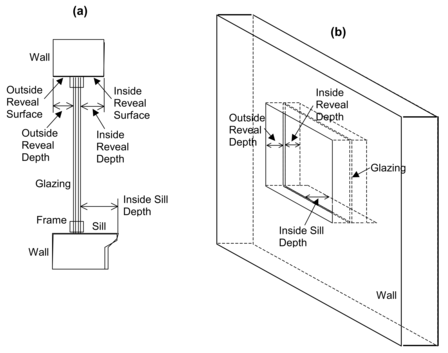
\includegraphics[width=0.9\textwidth, height=0.9\textheight, keepaspectratio=true]{media/image064.png}
\caption{(a) Vertical section through a window (with frame) showing outside and inside reveal surfaces and inside sill. (b) Perspective view looking from the outside of a window (without frame) showing reveal surfaces. Note that “Outside Reveal Depth” is not a user input; it is calculated by the program from the window and wall vertices. \protect \label{fig:a-vertical-section-through-a-window-with}}
\end{figure}

An IDF example:

\begin{lstlisting}

  WindowProperty:FrameAndDivider,
        TestFrameAndDivider, ! Frame/Divider Name
        0.05, ! Frame Width
        0.04, ! Frame Outside Projection
        0.03, ! Frame Inside Projection
        5.0,  ! Frame Conductance
        1.3,  ! Ratio of Frame-Edge Glass Conductance to Center-Of-Glass Conductance
        0.8,  ! Frame Solar Absorptance
        0.8,  ! Frame Visible Absorptance
        0.9,  ! Frame Thermal Emissivity
        DividedLite, ! Divider Type
        0.03, ! Divider Width
        2,    ! Number of Horizontal Dividers
        2,    ! Number of Vertical Dividers
        0.03, ! Divider Outside Projection
        0.03, ! Divider Inside Projection
        5.0,  ! Divider Conductance
        1.3,  ! Ratio of Divider-Edge Glass Conductance to Center-Of-Glass Conductance
        0.8,  ! Divider Solar Absorptance
        0.8,  ! Divider Visible Absorptance
        0.9,  ! Divider Thermal Emissivity
        0.7,  ! Outside Reveal Solar Absorptance
        0.25, ! Inside Sill Depth (m)
        0.6,  ! Inside Sill Solar Absorptance
        0.2,  ! Inside Reveal Depth (m)
        0.5;  ! Inside Reveal Solar Absorptance
\end{lstlisting}

\subsection{WindowProperty:AirflowControl}\label{windowpropertyairflowcontrol}

This object is used to specify the control mechanism for windows in which forced air flows in the gap between adjacent layers of glass. Such windows are called ``airflow windows.'' They are also known as ``heat-extract windows'' or ``climate windows.''

A common application is to reduce the zone load by exhausting indoor air through the window. In the cooling season this picks up and expels some of the solar heat absorbed by the window glass (and by the between-glass shade or blind, if present). In the heating season this warms the window, reducing the heat loss from the window. A side benefit is increased thermal comfort. This is because the inside surface of the window will generally be cooler in summer and warmer in winter.

The surface output variable ``Surface Window Gap Convective Heat Transfer Rate'' gives the heat picked up (or lost) by the gap airflow.

\subsubsection{Inputs}\label{inputs-34-001}

\paragraph{Field: Name}\label{field-name-31-001}

Name of the window that this WindowProperty:AirflowControl refers to. It must be a window with two or three glass layers, i.e., double- or triple-glazing. For triple-glazing the airflow is assumed to be between the two inner glass layers.

An error will result if the gas in the airflow gap is other than air. If an airflow window has a between-glass shade or blind, the gas in the gap on either side of the shade or blind must be air.

\paragraph{Field: Airflow Source}\label{field-airflow-source}

The source of the gap airflow. The choices are:

\emph{IndoorAir}: Indoor air from the window's zone is passed through the window.

\emph{OutdoorAir}: Outdoor air is passed through the window.

\paragraph{Field: Airflow Destination}\label{field-airflow-destination}

This is where the gap air goes after passing through the window. The choices are:

\emph{IndoorAir}: The gap air goes to the indoor air of the window's zone.

\emph{OutdoorAir}: The gap air goes to the outside air.

\emph{ReturnAir}. The gap air goes to the return air for the window's zone. This choice is allowed only if Airflow Source = InsideAir. If the return air flow is zero, the gap air goes to the indoor air of the window's zone. If the sum of the gap airflow for all of the windows in a zone with Airflow Destination = ReturnAir exceeds the return airflow, then the difference between this sum and the return airflow goes to the indoor air. The name of the Return Air Node may be specified below.

Figure~\ref{fig:gap-airflow-configurations-for-airflow} shows the allowed combinations of Airflow Source and Airflow Destination. The allowed combinations of Airflow Source and Airflow Destination are:

IndoorAir -\textgreater{} OutdoorAir

IndoorAir -\textgreater{} IndoorAir

IndoorAir -\textgreater{} ReturnAir

OutdoorAir -\textgreater{} IndoorAir

OutdoorAir -\textgreater{} OutdoorAir

\paragraph{Field: Maximum Flow Rate}\label{field-maximum-flow-rate-003}

The maximum value of the airflow, in m\(^{3}\)/s per m of glazing width. The value is typically 0.006 to 0.009 m\(^{3}\)/s-m (4 to 6 cfm/ft).

The airflow can be modulated by specifying Airflow Has Multiplier Schedule = Yes and giving the name of the Airflow Multiplier Schedule (see below).

The fan energy used to move the air through the gap is generally very small and so is ignored.

\paragraph{Field: Airflow Control Type}\label{field-airflow-control-type}

Specifies how the airflow is controlled. The choices are:

\emph{AlwaysOnAtMaximumFlow}. The airflow is always equal to Maximum Airflow.

\emph{AlwaysOff}. The airflow is always zero.

\emph{ScheduledOnly}. The airflow in a particular timestep equals Maximum Airflow times the value of the Airflow Multiplier Schedule for that timestep.

\paragraph{Field: Airflow Is Scheduled}\label{field-airflow-is-scheduled}

Specifies if the airflow is scheduled. The choices are:

\emph{Yes}. The airflow is scheduled.

\emph{No}. The airflow is not scheduled.

If Yes, Airflow Multiplier Schedule Name is required.

\paragraph{Field: Airflow Multiplier Schedule Name}\label{field-airflow-multiplier-schedule-name}

The name of a schedule with values between 0.0 and 1.0. The timestep value of the airflow is Maximum Airflow times the schedule value. Required if Airflow Is Scheduled = Yes. Unused if Airflow Is Scheduled = No. This schedule should have a ScheduleType with Numeric Type = Continuous and Range = 0.0 : 1.0.

\paragraph{Field: Airflow Return Air Node Name}\label{field-airflow-return-air-node-name}

The name of the return air node for this airflow window if the Airflow Destination is ReturnAir. If left blank, this defaults to the first return air node for the zone containing the window surface.

\begin{figure}[hbtp] % fig 39
\centering
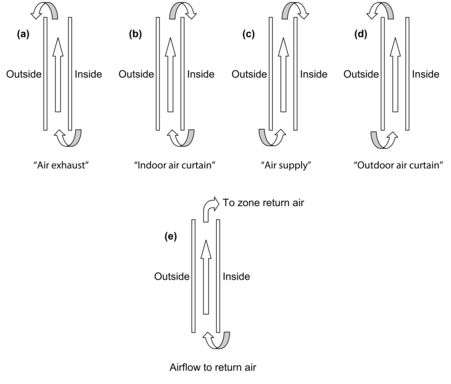
\includegraphics[width=0.9\textwidth, height=0.9\textheight, keepaspectratio=true]{media/image065.png}
  \caption{Gap airflow configurations for airflow windows. (a) \textbf{Air exhaust window}: Airflow Source = InsideAir, Airflow Destination = OutsideAir; (b) \textbf{Indoor air curtain window}: Airflow Source = InsideAir, Airflow Destination = InsideAir; (c) \textbf{Air supply window}: Airflow Source = OutsideAir, Airflow Destination = InsideAir; (d) \textbf{Outdoor air curtain window}: Airflow Source = OutsideAir, Airflow Destination = OutsideAir; (e) \textbf{Airflow to Return Air}: Airflow Source = InsideAir, Airflow Destination = ReturnAir. Based on ``Active facades,'' Version no. 1, Belgian Building Research Institute, June 2002. \protect \label{fig:gap-airflow-configurations-for-airflow}}
\end{figure}

An IDF example: window with a constant airflow from inside to outside at 0.008 m\(^{3}\)/s-m.

\begin{lstlisting}
WindowProperty:AirflowControl,
      Zn001:Wall001:Win002,   !- Name
      InsideAir,              !- Airflow Source
      OutsideAir,             !- Airflow Destination
      0.008,                  !- Maximum Flow Rate {m3/s-m}
      AlwaysOnAtMaxFlow,      !- Airflow Control Type
      No,                     !- Airflow Is Scheduled
      ;                       !- Airflow Multiplier Schedule Name
      ,                       !- Airflow Return Air Node Name
\end{lstlisting}

\subsection{WindowProperty:StormWindow}\label{windowpropertystormwindow}

This object allows you to assign a movable exterior glass layer (``storm window'' or ``storm glass'') that is usually applied to a window in the winter to reduce heat loss and removed in the summer. A WindowProperty:StormWindow object is required for each window that has an associated storm window. It is assumed that:

\begin{itemize}
\item
  When the storm glass is in place it is the outermost layer of the window, it covers only the glazed part of the window and not the frame, and it forms a tight seal. See Figure~\ref{fig:section-through-a-single-glazed-window}.
\item
  When the storm glass is not in place it is completely removed and has no effect on window heat transfer.
\item
  The gap between the storm glass and rest of the glazing is filled with air.
\end{itemize}

\begin{figure}[hbtp] % fig 40
\centering
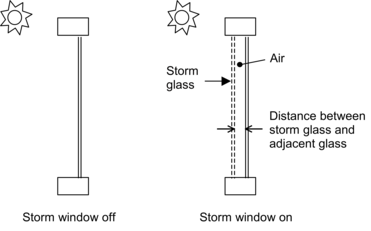
\includegraphics[width=0.9\textwidth, height=0.9\textheight, keepaspectratio=true]{media/image066.png}
\caption{Section through a single-glazed window without (left) and with (right) a storm glass layer. Not to scale. \protect \label{fig:section-through-a-single-glazed-window}}
\end{figure}

With the addition of a storm window, single glazing effectively becomes double glazing, double glazing becomes triple glazing, etc.

The presence of a storm window is indicated by the output variable ``Surface Storm Window On Off Status'' (see ``Window Output Variables''). This flag is \textbf{0} if the storm window is off, \textbf{1} if it is on, and \textbf{--1} if the window does not have an associated storm window.

The program automatically creates a window construction (ref: Construction) that consists of the storm window glass layer and its adjacent air layer added to the original (unshaded, or ``bare'') window construction. In the eplusout.eio file this construction is called BARECONSTRUCTIONWITHSTORMWIN:\emph{n}, where \emph{n} is the number of the associated StormWin object. If the window has a shaded construction, the program creates a construction called SHADEDCONSTRUCTIONWITHSTORMWIN:\emph{n} that consists of the storm window glass layer and its adjacent air layer added to the original shaded window construction.

The program also creates a WindowMaterial:Gas layer corresponding to the air layer adjacent to the storm glass. In the eplusout.eio file this layer is called AIR:STORMWIN:\emph{k}MM, where \emph{k} is the thickness of the air layer expressed as an integer number of millimeters.

\subsubsection{Inputs}\label{inputs-35-001}

\paragraph{Field: Window Name}\label{field-window-name-000}

This is the name of a window (or glass door) to which the storm glass is applied. Not all windows can accept WindowProperty:StormWindow. The rules are:

\begin{itemize}
\item
  The window must be an exterior window. WindowProperty:StormWindow is not applicable to interior (interzone) windows.
\item
  The window construction (without the storm glass layer) can have up to three glass layers.
\item
  If the window has an associated shaded construction (ref: WindowShadingControl), that construction can have an interior shade or blind and up to three glass layers, or a between-glass shade or blind and two glass layers. The shaded construction cannot have an exterior shade or blind, cannot have a between-glass shade or blind and three glass layers, and cannot be switchable glazing.
\item
  The window cannot be an airflow window, i.e., a window that has an associated WindowProperty:AirflowControl.
\end{itemize}

\paragraph{Field: Storm Glass Layer Name}\label{field-storm-glass-layer-name}

This is the name of a window glass material. Storm windows are assumed to consist of a single layer of glass. A storm window frame, if present, is ignored.

\paragraph{Field: Distance Between Storm Glass Layer and Adjacent Glass}\label{field-distance-between-storm-glass-layer-and-adjacent-glass}

The separation between the storm glass and the rest of the window (Figure~\ref{fig:section-through-a-single-glazed-window}). It is measured from the inside of the storm glass layer to the outside of the adjacent glass layer.

\paragraph{Field: Month that Storm Glass Layer Is Put On}\label{field-month-that-storm-glass-layer-is-put-on}

The number of the month (January = 1, February = 2, etc.) during which the storm window is put in place.

\paragraph{Field: Day of Month that Storm Glass Layer Is Put On}\label{field-day-of-month-that-storm-glass-layer-is-put-on}

The day of the month that the storm window is put in place. It is assumed that the storm window is put in place at the beginning of this day, i.e., during the first simulation timestep of the day, and remains in place until that month and day given by the following two fields.

\paragraph{Field: Month that Storm Glass Layer Is Taken Off}\label{field-month-that-storm-glass-layer-is-taken-off}

The number of the month (January = 1, February = 2, etc.) during which the storm window is removed.

\paragraph{Field: Day of Month that Storm Glass Layer Is Taken Off}\label{field-day-of-month-that-storm-glass-layer-is-taken-off}

The day of the month that the storm window is removed. It is assumed that the storm window is removed at the beginning of this day, i.e., during the first simulation timestep of the day, and stays off until the month and day given by Month that Storm Glass Layer Is Put On, Day of Month that Storm Glass Layer Is Put On.

In the northern hemisphere, the month the storm window is put on is generally greater than the month it is taken off (for example put on in month 10, when it starts to get cold, and taken off in month 5, when it starts to warm up). In the southern hemisphere this is reversed: month on is less than month off.

An IDF example of WindowProperty:StormWindow. The storm window is put in place on October 15 and removed on May 1.

\begin{lstlisting}
WindowProperty:StormWindow,
   Window1, !- Name of Window to Which Storm Window Glass Layer is Applied
   GlassA,  !- Name of Material:WindowGlass or MATERIAL:WindowGlass:AltInput that is the storm window layer
   0.060,   !- Distance from storm window to adjacent glass (m)
   10,      !- Month that Storm Window Is Put On
   15,      !- Day of Month that Storm Window Is Put On
   5,       !- Month that Storm Window Is Taken Off
   1;       !- Day of Month that Storm Window Is Taken Off
\end{lstlisting}

\subsection{Importing Windows from WINDOW program}\label{importing-windows-from-window-program}

\begin{callout}
WINDOW v6.3 and later is capable of writing IDF excerpts for Window data. This is the preferred method as no external file is necessary. See the Tips document for details on obtaining the IDF excerpt.
\end{callout}

The WINDOW program calculates the U-value, Solar Heat Gain Coefficient, solar transmission/absorption characteristics, visible transmission characteristics and other properties of a window under standard indoor and outdoor conditions. WINDOW treats the whole window system---glazing, frame and divider. A sub-program of WINDOW called THERM uses a 2-D finite element calculation to determine the effective conductance of frame, divider and edge-of-glass elements. Another sub-program, OPTICS, determines the solar-optical properties of glazing, including laminates and coated glass.

WINDOW can write a data file containing a description of the window that was analyzed. An example of this file (which is no longer the preferred method) is shown in the Tips document under WINDOW generated files. is shown below. This file, which can be named by the user, can be read by EnergyPlus. For more complete description and examples, see the object description -- Construction:WindowDataFile.

In this way, the same window that was created in WINDOW can be imported into EnergyPlus for annual energy analysis without having to re-input the window data. To obtain WINDOW, THERM, or OPTICS go to \url{http://windows.lbl.gov} and choose the software link. A major advantage of using WINDOW to create window input for EnergyPlus is that you will have direct access to WINDOW's expanding database of over 1000 different glass types; and you will be able to browse through this database according to different criteria (color, transmittance, solar heat gain coefficient, etc.) to help you select the best glass type for your application.

Although WINDOW writes only one window entry on the WINDOW data file, EnergyPlus users can combine two or more of these files to end up with a single data file with multiple window entries of different types. In this way a library of windows from WINDOW can be built up if so desired. If you combine files like this you should be sure not to leave out or change any of lines from the original files.

There are four methods for inputting window constructions in EnergyPlus:

\begin{enumerate}
\tightlist
\item
  input full spectral data for each layer in the IDF,
\item
  input spectral average data for each layer in the IDF,
\item
  items 1 and 2 can be accomplished by reporting the IDF excerpt method from WINDOW
\item
  import WINDOW report containing layer-by-layer calculated values and overall glazing system angular values.
\end{enumerate}

\begin{callout}
  \warning{Note: When using method 4, the overall glazing system angular dependent properties, including Tsol, Abs, Rfsol, Rbsol, Tvis, Rfvis, and Rbvis, are not used by EnergyPlus. Therefore, methods 1 and 2 and preferably 3 are recommended.}
\end{callout}

\begin{itemize}
\item
  The SHGC calculations in EnergyPlus for window layers input using full spectral data use a spectral weighting data set (derived from Optics5 data file ISO-9845GlobalNorm.std) that is different from the WINDOW default spectral weighting data set (W5\_NFRC\_2003.std). This difference accounts for most of the variation in SHGC values reported by EnergyPlus and WINDOW for full spectral data window layer input. This variation is more pronounced for window constructions of three glass layers or more.
\item
  Users intending to select a window construction based on SHGC value for energy code compliance should base their selection on the value reported by WINDOW since this is the officially recognized value.
\end{itemize}

In EnergyPlus, the Window data file is searched for each ``Construction:WindowDataFile'' object in the EnergyPlus input. This object has a very simple form:

\begin{lstlisting}
Construction:WindowDataFile,
  ConstructionName,
  FileName; ! Default is Window5DataFile.dat in the "run" folder.
\end{lstlisting}

If there is a window called ConstructionName on the Window data file, the data for that window is read from the file and the following EnergyPlus objects and their names are created. The ``W5'' prefixed to these names indicates that the object originated in the Window data file.

\subsection{Using LBNLs Windows Calculation Engine}
This is new windows simulation engine that will be used in both EnergyPlus and Berkeley Lab WINDOW. The intent is for this engine to replace all other window calculation modules in EnergyPlus. For the time being, other modules will still be available. To use the new Window Calculation Engine, insert the following into IDF:

 \begin{lstlisting}
 WindowsCalculationEngine,
 ExternalWindowsModel;
 \end{lstlisting}

\subsection{Zone Thermal Output(s)}\label{zone-thermal-outputs-1}

In addition to the canned Surface reports (view the Reports section later in this document) and surface variables (above), the following variables are available for all zones:

\begin{lstlisting}
Zone,Sum,Zone Total Internal Radiant Heating Energy [J]
Zone,Sum,Zone Total Internal Visible Radiation Heating Energy [J]
Zone,Sum,Zone Total Internal Convective Heating Energy [J]
Zone,Sum,Zone Total Internal Latent Gain Energy [J]
Zone,Sum,Zone Total Internal Total Heating Energy [J]
Zone,Average,Zone Mean Air Temperature [C]
HVAC,Average,Zone Air Temperature [C]
Zone,Average,Zone Mean Radiant Temperature [C]
Zone,Average,Zone Operative Temperature [C]
HVAC,Sum,Zone Air System Sensible Heating Energy [J]
HVAC,Sum,Zone Air System Sensible Cooling Energy [J]
HVAC,Average,Zone Air System Sensible Heating Rate [W]
HVAC,Average,Zone Air System Sensible Cooling Rate [W]
HVAC,Average,Zone Air Humidity Ratio[kgWater/kgDryAir]
HVAC,Average,Zone Air Relative Humidity[%]
\end{lstlisting}

Two of these are of particular interest:

\begin{lstlisting}
Zone,Average,Zone Mean Air Temperature [C]
HVAC,Average,Zone Air Temperature [C]
\end{lstlisting}

These two variable outputs are/should be identical. However, note that they can be reported at different time intervals. ``Zone Mean Air Temperature'' is only available on the Zone/HB timestep (Number of Timesteps per Hour) whereas ``Zone Air Temperature'' can be reported at the HVAC timestep (which can vary).

\subsubsection{Zone Mean Air Temperature {[}C{]}}\label{zone-mean-air-temperature-c-1}

From the code definition, the zone mean air temperature is the average temperature of the air temperatures at the system timestep. Remember that the zone heat balance represents a ``well stirred'' model for a zone, therefore there is only one mean air temperature to represent the air temperature for the zone.

\subsubsection{Zone Air Temperature {[}C{]}}\label{zone-air-temperature-c-1}

This is very similar to the mean air temperature in the last field. The ``well stirred'' model for the zone is the basis, but this temperature is also available at the ``detailed'' system timestep.

\subsubsection{Zone Mean Radiant Temperature {[}C{]}}\label{zone-mean-radiant-temperature-c-1}

The Mean Radiant Temperature (MRT) in degrees Celsius of a space is really the measure of the combined effects of temperatures of surfaces within that space. The larger the surface area and the closer one is to it, the more effect the surface temperature of that surface has on each other. The MRT is the measure of all these surface areas and temperatures.

\subsubsection{Zone Operative Temperature {[}C{]}}\label{zone-operative-temperature-c-1}

Zone Operative Temperature (OT) is the average of the Zone Mean Air Temperature (MAT) and Zone Mean Radiant Temperature (MRT), OT = 0.5*MAT + 0.5*MRT. This output variable is not affected by the type of thermostat controls in the zone, and does not include the direct effect of high temperature radiant systems.~ See also Zone Thermostat Operative Temperature.

\subsubsection{Zone Air System Sensible Heating Energy {[}J{]}}\label{zone-air-system-sensible-heating-energy-j-1}

This field represents the sensible heating energy in Joules that is actually supplied by the system to that zone for the timestep reported. This is the sensible heating rate multiplied by the simulation timestep. This is calculated and reported from the Correct step in the Zone Predictor-Corrector module. This field is not multiplied by zone or group multipliers.

\begin{callout}
Zone Air System Sensible Heating (and Cooling) Energy (and Rate) all report the heating or cooling delivered by the HVAC system to a zone. These values are calculated by multiplying the supply air mass flow rate by the difference between the supply air temperature and the zone air temperature. This does not always indicate the operation of heating or cooling coils. For example, cooling will be reported if the supply air is cooled due to the introduction of outside air, even if all coils are off.

Note that these variables are calculated at the system timestep. When reported at the ``detailed'' reporting frequency, these variable will never show heating and cooling both in the same system timestep. If reported at a frequency less than ``Detailed'' (for example, Hourly) values may appear in both the heating and cooling variable for the same hour if the system cooled the zone for part of the reporting period and heated the zone for another part of the reporting period.
\end{callout}

\subsubsection{Zone Air System Sensible Cooling Energy {[}J{]}}\label{zone-air-system-sensible-cooling-energy-j-1}

This field represents the sensible cooling energy in Joules that is actually supplied by the system to that zone for the timestep reported. This is the sensible cooling rate multiplied by the simulation timestep. This is calculated and reported from the Correct step in the Zone Predictor-Corrector module. This field is not multiplied by zone or group multipliers.

\subsubsection{Zone Air System Sensible Heating Rate {[}W{]}}\label{zone-air-system-sensible-heating-rate-w-1}

This field represents the sensible heating rate in Watts that is actually supplied by the system to that zone for the timestep reported. This is calculated and reported from the Correct step in the Zone Predictor-Corrector module. This field is not multiplied by zone or group multipliers. The Zone Air System Sensible Heating Rate may not agree exactly with the equipment-level delivered energy transfer rate when the zone temperature is changing significantly over a timestep (e.g. during thermostat setback and setup), but the energy will balance out over time.

\subsubsection{Zone Air System Sensible Cooling Rate {[}W{]}}\label{zone-air-system-sensible-cooling-rate-w-1}

This field represents the sensible cooling rate in Watts that is actually supplied by the system to that zone for the timestep reported. This is calculated and reported from the Correct step in the Zone Predictor-Corrector module. This field is not multiplied by zone or group multipliers. The Zone Air System Sensible Cooling Rate may not agree exactly with the equipment-level delivered energy transfer rate when the zone temperature is changing significantly over a timestep (e.g. during thermostat setback and setup), but the energy will balance out over time.

\subsubsection{Zone Air Humidity Ratio{[}kgWater/kgDryAir{]}}\label{zone-air-humidity-ratiokgwaterkgdryair}

This field represents the air humidity ratio after the correct step for each zone. The humidity ratio is the mass of water vapor to the mass of dry air contained in the zone in (kg water/kg air) and is unitless.

\subsubsection{Zone Air Relative Humidity{[}\%{]}}\label{zone-air-relative-humidity-1}

This field represents the air relative humidity ratio after the correct step for each zone. The relative humidity is in percent and uses the Zone Air Temperature, the Zone Air Humidity Ratio and the Outside Barometric Pressure for calculation.

\subsubsection{Zone Total Internal Radiant Heating Energy {[}J{]}}\label{zone-total-internal-radiant-heating-energy-j-1}

This field represents the sum of radiant gains from specific internal sources (e.g.~equipment) throughout the zone in joules. This includes radiant gain from People, Lights, Electric Equipment, Gas Equipment, Other Equipment, Hot Water Equipment, and Steam Equipment.

\subsubsection{Zone-Total Internal Visible Heat Gain {[}J{]}}\label{zone-total-internal-visible-heat-gain-j}

This field expresses the sum of heat gain in joules that is the calculated short wavelength radiation gain from lights in the zones. This calculation uses the total energy from lights and the fraction visible to realize this value, summed over the zones in the simulation.

\subsubsection{Zone Total Internal Convective Heating Energy {[}J{]}}\label{zone-total-internal-convective-heating-energy-j-1}

This field represents the sum of convective gains from specific sources (e.g.~equipment) throughout the zone in joules. This includes convective gain from People, Lights, Electric Equipment, Gas Equipment, Other Equipment, Hot Water Equipment, and Steam Equipment.

\subsubsection{Zone Total Internal Latent Gain Energy {[}J{]}}\label{zone-total-internal-latent-gain-energy-j-1}

This field represents the sum of latent gains from specific internal sources (e.g.~equipment) throughout the zone in joules. This includes latent gain from People, Electric Equipment, Gas Equipment, Other Equipment, Hot Water Equipment, and Steam Equipment.

\subsubsection{Zone Total Internal Total Heating Energy {[}J{]}}\label{zone-total-internal-total-heating-energy-j-1}

This field represents the sum of all heat gains throughout the zone in joules. This includes all heat gains from People, Lights, Electric Equipment, Gas Equipment, Other Equipment, Hot Water Equipment, and Steam Equipment.
